% !Mode:: "Tex:UTF-8"

\section{Distribución muestral. Segunda versión del Teorema Central del Límite.}
\label{cap06:sec:DistribucionMuestralTCL2}

Nuestro primer objetivo es tratar de entender, en el caso más elemental
posible, lo que la Teoría de la Probabilidad tiene que decir sobre el proceso
de muestreo. Para ello, vamos a empezar con un largo ejemplo, que va a
ocupar casi toda la primera sección de este capítulo. Y de hecho, seguiremos usando el que es casi
nuestro ejemplo canónico: vamos a lanzar dados. Ya hemos tenido ocasión de
comprobar, por ejemplo en el Capítulo \ref{cap:TeoremaCentralLimite}, que estos
ejemplos son suficientemente simples como para permitirnos comprobar si
nuestras ideas van bien encaminadas, pero a la vez nos permiten en ocasiones
extraer conclusiones profundas.  El ejemplo que vamos a ver a continuación es,
con certeza, uno de los más importantes, si no el más importante del curso. Nos
atrevemos a decir que no se puede entender para qué sirve la Estadística si no
se ha entendido al menos el mensaje básico de este ejemplo. La lectura del
ejemplo será laboriosa, y seguramente será necesaria al menos una relectura.
Pero a cambio le aseguramos al lector que está a punto de asomarse a una idea
verdaderamente profunda.
\begin{ejemplo}
\label{cap06:ejem:DistribucionMediaMuestral}
    Consideremos la variable aleatoria $X(a,b)=a+b$ que representa la suma de puntos obtenidos al
    lanzar dos dados. Recordemos que el espacio muestral subyacente tiene 36 sucesos elementales
    equiprobables, que podemos representar como
        \[d_1=(1,1), d_2=(1,2),\ldots,d_6=(1,6),d_7=(2,1)\mbox{ y así hasta el }d_{36}=(6,6).\]
    Para ayudarte a seguir la notación y la discusión de este ejemplo, la Figura
    \ref{cap06:fig:EjemploEspacioMuestral2Dados} muestra un diagrama, que trata de aclarar los
    conceptos que van a ir apareciendo.

    Ya vimos (en el Ejemplo \ref{cap04:ejem:VariablesAleatoriasEliminanInformacion}, página
    \pageref{cap04:ejem:VariablesAleatoriasEliminanInformacion}) la función o tabla de densidad de
    probabilidad de esta variable, que aquí reproducimos como Tabla
    \ref{cap06:tabla:probabilidadSumaDados}. La Figura \ref{cap06:fig:distribucionXDosDados}
    muestra esta misma distribución de probabilidad mediante un diagrama de columnas. Como puede
    verse, la distribución tiene forma de v invertida, ya que la probabilidad aumenta o disminuye
    siempre en la mima cantidad, $1/36$. La figura muestra frecuencias en lugar de probabilidades,
    pero eso no afecta  a la {\em forma} del diagrama, porque las probabilidades se obtienen de las
    frecuencias dividiendo por 36, así que se trataría de un simple cambio de escala en el eje
    vertical.

\begin{figure}[p]
\begin{center}
\begin{enColor}
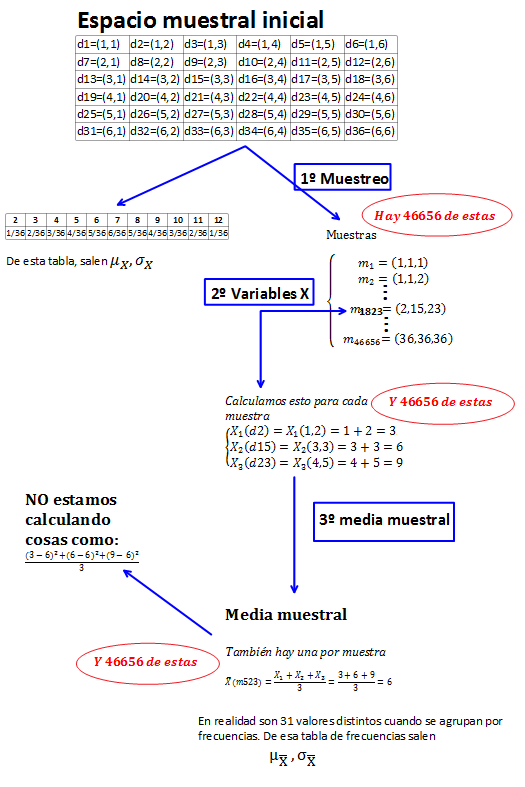
\includegraphics[width=13cm]{../fig/cap06-DiagramaMuestreoDosDados.png}
\end{enColor}
\begin{bn}
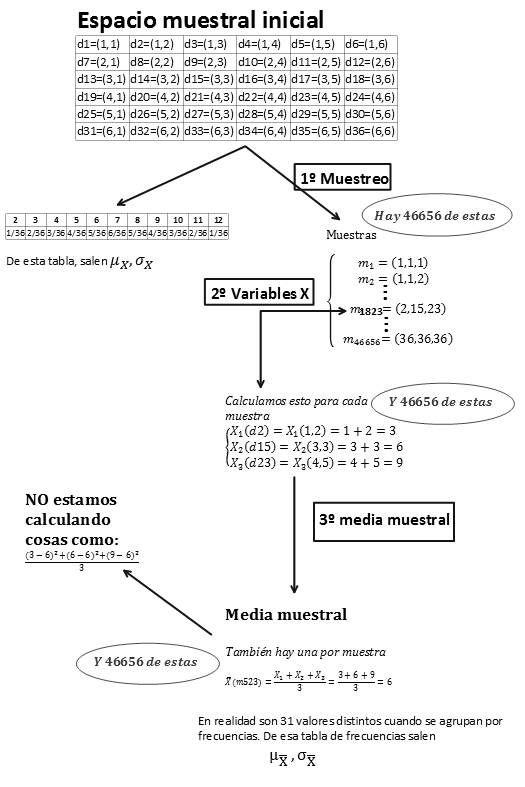
\includegraphics[width=13cm]{../fig/cap06-DiagramaMuestreoDosDados-bn.png}
\end{bn}
\caption{Diagrama del espacio muestral asociado  al lanzamiento de  dos dados.}
\label{cap06:fig:EjemploEspacioMuestral2Dados}
\end{center}
\end{figure}



    \begin{table}[ht]
    \begin{center}
    {\small
    \begin{tabular}[t]{|c|c|c|c|c|c|c|c|c|c|c|c|}
    \hline
    \begin{minipage}{2cm}
    \rule{0cm}{0.5cm}{\em Valor de\\ la suma:\\}
    \end{minipage}
    &2&3&4&5&6&7&8&9&10&11&12\\
    \hline
    \begin{minipage}{2cm}
    {\em Probabilidad\\
    de ese valor:}
    \end{minipage}
    &\rule{0cm}{0.7cm}$\dfrac{1}{36}$&$\dfrac{2}{36}$&$\dfrac{3}{36}$&$\dfrac{4}{36}$&$\dfrac{5}{36}$&$\dfrac{6}{36}$&$\dfrac{5}{36}$&$\dfrac{4}{36}$&$\dfrac{3}{36}$&$\dfrac{2}{36}$&$\dfrac{1}{36}$\\
    &&&&&&&&&&&\\
    \hline
    \end{tabular}
    }
    \caption{Probabilidad de las posibles sumas al lanzar dos dados}\label{cap06:tabla:probabilidadSumaDados}
    \end{center}
    \end{table}


\begin{figure}[h!]
\begin{center}
\begin{enColor}
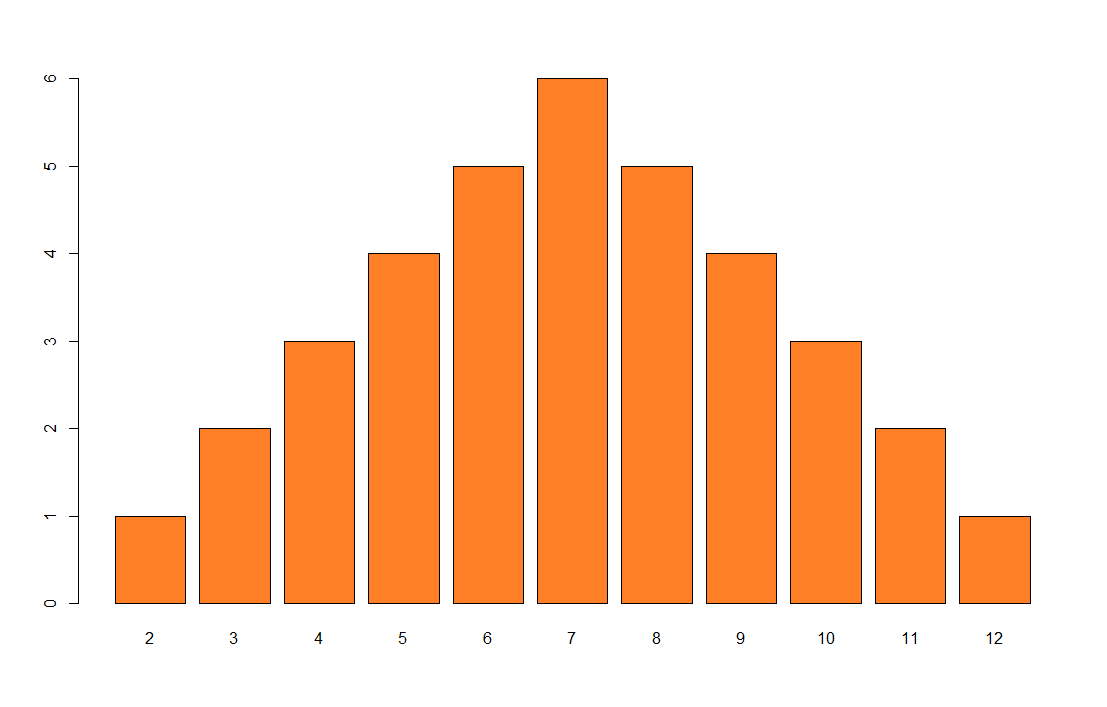
\includegraphics[width=12cm]{../fig/cap06-DistribucionOriginalVsMuestral-01.png}\\
\end{enColor}
\begin{bn}
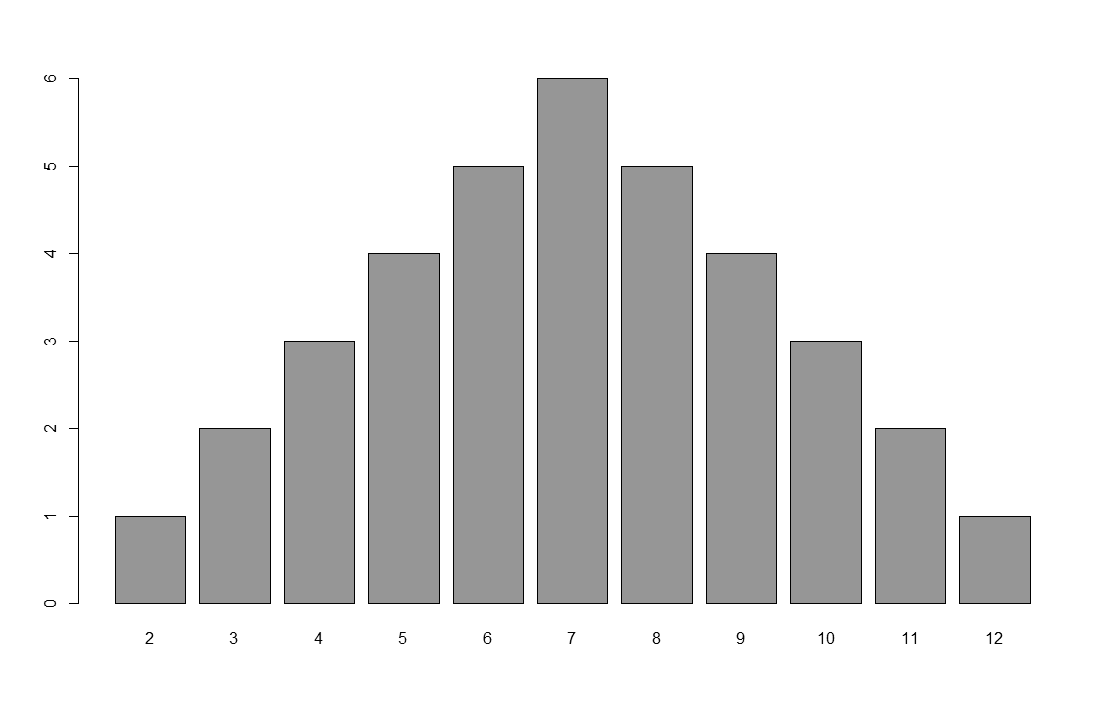
\includegraphics[width=12cm]{../fig/cap06-DistribucionOriginalVsMuestral-01-bn.png}\\
\end{bn}
\caption{Distribución de la variable $X$, suma al lanzar dos dados.}
\label{cap06:fig:distribucionXDosDados}
\end{center}
\end{figure}

    A partir de la tabla \ref{cap06:tabla:probabilidadSumaDados} es fácil calcular la media y la
    desviación típica de $X$ (ya lo hicimos, ver los Ejemplos
    \ref{ejem:Cap04:VariableAleatoriaSumaDosDadosMedia} y
    \ref{cap04:ejem:varianzaVariableAleatoriaDiscreta}). Se obtiene $\mu_X=7$,
    $\sigma_X=\dfrac{\sqrt{35}}{6}\approx 2.415$. Naturalmente, en un caso como este, en que el
    espacio muestral tiene sólo 36 elementos, y conocemos todos los detalles, el proceso de
    muestreo es innecesario. Pero precisamente por eso nos interesa este ejemplo, por ser tan
    sencillo. Vamos a usarlo como un modelo  ``de juguete'', como un laboratorio en el que aclarar
    nuestras ideas sobre las implicaciones del proceso de muestreo. Según nuestra experiencia, la
    mayoría de los lectores se van a llevar alguna sorpresa.

    Así pues, pensemos en muestras. En particular, vamos a pensar en muestras de tamaño 3. ¿Cuántas
    muestras distintas de tamaño 3 podemos obtener? Hay 36 resultados distintos posibles al lanzar
    dos dados, los que hemos llamado $d_1,d_2,\ldots,d_{36}$.  Así que una muestra puede ser
    cualquier terna tal como
        \[(d_2,d_{15},d_{23})\]
    que corresponde a los tres resultados
        \[d_2=(1,2), d_{15}=(3,3), d_{23}=(4,5)\]
    de los dados. Pero, ¿qué sucede con, por ejemplo, $(d_4,d_4,d_4)$? ¿Es esta una muestra que
    debamos tomar en consideración? ¿Debemos admitir valores repetidos? Hay que andar con cuidado
    aquí: es importante, para empezar, que los tres valores de la muestra sean independientes entre
    sí. Y eso obliga a considerar extracción con reemplazamiento. ¿Qué queremos decir con esto? Es
    como si tuviéramos una urna con bolas marcadas del 1 al 36 y aleatoriamente extrajéramos tres.
    Si después de cada extracción no devolvemos la bola, {!`}es evidente que los resultados de la
    segunda extracción no son independientes de los de la primera! Así que tenemos que devolver la
    bola a la caja cada vez. Y eso significa que sí, que tenemos que considerar muestras con
    repeticiones. Ahora ya podemos contestar a la pregunta de cuántas muestras de tres elementos
    hay. Son
    \[36^3=46656\]
    muestras distintas\footnote{Si no incluimos las repeticiones serían $\binom{36}{3}=7140$
    muestras distintas.} Visto de otra manera, se trata del número de variaciones con repetición de
    $36$ elementos tomados de $3$ en $3$. En el Tutorial06 aprenderemos a usar el ordenador para construir esas 46656 muestras, para que así el lector pueda comprobar todas las cuentas de este ejemplo,
    sin necesidad de fiarse sólo de nuestra palabra (a cambio, tendrá que fiarse del trabajo de un equipo de  programadores...). El procedimiento de muestreo que estamos utilizando presupone que {\sf
    esas $46656$ muestras son equiprobables.} Es como si metiéramos en una caja una colección de
    $46656$ fichas numeradas, las agitáramos bien, y extrajéramos una al azar.

    Para aprovechar a fondo este ejemplo, es importante detenerse a tener en cuenta que hemos
    empezado con un espacio muestral de tan sólo 36 valores, y que estamos tomando muestras de
    tamaño 3. En realidad, al considerar el proceso de muestreo, hemos creado un nuevo espacio
    muestral, de un tamaño mucho mayor que el original: el conjunto de las 46656 muestras posibles.
    Esas 46656 muestras de tamaño 3 van desde:
    \[m_1=(d_1,d_1,d_1),m_2=(d_1,d_1,d_2),\ldots,\mbox{ pasando por }m_{1823}=(d_2,d_{15},d_{23}),\]\[\ldots\mbox{ hasta }m_{46656}=(d_{36},d_{36},d_{36}).\]
    Es decir, volviendo por un momento a los resultados originales de los dos dados, la lista va
    desde
    \[m_1=\bigl((1,1),(1,1),(1,1)\bigr), \quad{\mbox{ tres dobles unos,}}\]
    hasta
    \[m_{46656}=\bigl((6,6),(6,6),(6,6)\bigr), \quad{\mbox{ tres dobles seises},}\]
    pasando, por supuesto, por
    \[m_{1823}=\bigl((1,2), (3,3), (4,5)\bigr).\]
    Cada una de estas muestras produce tres valores de ``sumas de los dos dados'' (tres valores de
    $X$). Cada muestra es una tirada (de dos dados), y vamos a llamar $X_1$ a la suma para la
    primera de las tres tiradas, y $X_2$ y $X_3$ a las sumas para la segunda y tercera tiradas,
    respectivamente.  Por ejemplo, para la muestra $(d_2,d_{15},d_{23})$, que vimos antes, esos
    tres valores, que vamos a llamar $X_1, X_2$ y $X_3$, son:
        \[X_1=\hspace{-3mm}\underbrace{1+2=3}_{\mbox{\small valor de $X(d_2)$}},\quad X_2=\hspace{-3mm}\underbrace{3+3=6}_{\mbox{\small valor de $X(d_{15})$}},
        \quad X_3=\hspace{-3mm}\underbrace{4+5=9}_{\mbox{\small valor de $X(d_{23})$}}.\] Cada una
    de estas $X_1$, $X_2$ y  $X_3$ es una variable aleatoria, pero además, cada una de ellas es una
    copia idéntica de $X$. Para ayudarnos a ver esto, pensemos en la descripción de $X=$``sumar el
    resultado de los dos dados'', y vemos que eso describe exactamente lo que hacen $X_1$, $X_2$ y
    $X_3$. Los hechos importantes que hay que retener son que, al ser iguales, las tres tienen la
    misma media y varianza que $X$, y que son independientes (gracias al muestreo con
    reemplazamiento, claro).


%
%
%        \begin{center}\label{fig:DiagramaDistribucionMediaMuestral}
%        \includegraphics[width=16cm]{../fig/2011-11-08-Diagrama.PNG}
%        \end{center}
%        {\LARGE La tabla de frecuencias de $\bar X$ está en la página \pageref{cap06:tabla:TablaFrecuenciasMediasMuestrales}}
%        \newpage

        A continuación, puesto que tenemos tres valores ($X_1$, $X_2$ y  $X_3$), podemos hacer la media de estos tres:
        \[\mbox{media de $X$ en la muestra $m_{1823}$ }=\dfrac{X_1+X_2+X_3}{3}=\dfrac{3+6+9}{3}=\dfrac{18}{3}=6.\]
        Esta media es lo que vamos a llamar la \index{media muestral}{\sf media muestral}, que representamos por $\bar X$. Así pues
        \[\bar X=\dfrac{X_1+X_2+X_3}{3},\mbox{ y por tanto }\bar X(d_2,d_{15},d_{23})=6.\]
        {!`}Es importante que no confundas los índices $(1,15,23)$ de la muestra $(d_2,d_{15},d_{23})$
        con $(3,6,9)$, que son los valores de las sumas para esas parejas de números! Asegúrate de entender esto antes de seguir adelante.

        Puesto que tenemos 46656 muestras distintas, podemos calcular 46656 de estas medias muestrales. Y podemos ver esos 46656 valores como una nueva variable aleatoria, que llamaremos, naturalmente $\bar X$. Si agrupamos los valores de $\bar X$ por frecuencias se obtiene la Tabla \ref{cap06:tabla:TablaFrecuenciasMediasMuestrales} (pág. \pageref{cap06:tabla:TablaFrecuenciasMediasMuestrales}). Las medias muestrales van desde el 2 al 12, en incrementos de $1/3$ que se deben, naturalmente, al tamaño 3 de la muestra.

    \begin{table}[hp]
        \begin{center}
        {\small
        \begin{tabular}{|c|c|}
        \hline
        {\bf Valor de $\bar X$}\rule{0cm}{0.7cm}&{\bf Frecuencia}\\
        \hline
        2& 1 \\ \hline
        2$+1/3$\rule{0cm}{0.35cm}&6 \\ \hline
        2$+2/3$\rule{0cm}{0.35cm}& 21 \\ \hline
        3&56 \\ \hline
        3$+1/3$\rule{0cm}{0.35cm}&126 \\ \hline
        3$+2/3$\rule{0cm}{0.35cm}&252 \\ \hline
        4& 456 \\ \hline
        4$+1/3$\rule{0cm}{0.35cm}&756 \\ \hline
        4$+2/3$\rule{0cm}{0.35cm}& 1161 \\ \hline
        5&1666 \\ \hline
        5$+1/3$\rule{0cm}{0.35cm}&2247 \\ \hline
        5$+2/3$\rule{0cm}{0.35cm}& 2856 \\ \hline
        6&3431 \\ \hline
        6$+1/3$\rule{0cm}{0.35cm}&3906 \\ \hline
        6$+2/3$\rule{0cm}{0.35cm}& 4221 \\ \hline
        7&4332 \\ \hline
        7$+1/3$\rule{0cm}{0.35cm}&4221 \\ \hline
        7$+2/3$\rule{0cm}{0.35cm}& 3906 \\ \hline
        8&3431 \\ \hline
        8$+1/3$\rule{0cm}{0.35cm}& 2856 \\ \hline
        8$+2/3$\rule{0cm}{0.35cm}& 2247 \\ \hline
        9&1666 \\ \hline
        9$+1/3$\rule{0cm}{0.35cm}& 1161 \\ \hline
        9$+2/3$\rule{0cm}{0.35cm}&756 \\ \hline
        10&456 \\ \hline
        10$+1/3$\rule{0cm}{0.35cm}&252 \\ \hline
        10$+2/3$\rule{0cm}{0.35cm}&126 \\ \hline
        11& 56 \\ \hline
        11$+1/3$\rule{0cm}{0.35cm}& 21 \\ \hline
        11$+2/3$\rule{0cm}{0.35cm}&6 \\ \hline
        12&1 \\ \hline
        TOTAL:&46656\\ \hline
        \end{tabular}
        }
        \end{center}
        \caption{Tabla de frecuencias de medias muestrales para el ejemplo de lanzamiento de dos dados}
        \label{cap06:tabla:TablaFrecuenciasMediasMuestrales}
    \end{table}

    Es conveniente dedicar unos segundos a estudiar los valores de esta tabla. La hemos escrito como una tabla de frecuencias, de veces que cada valor de $\bar X$ aparece repetido en las $46656$ muestras de tamaño $3$. Son frecuencias, pero podemos convertir las frecuencias en probabilidades, dividiéndolas por $46656$. Podríamos añadir esas probabilidades a la Tabla \ref{cap06:tabla:TablaFrecuenciasMediasMuestrales} pero, para entender la forma en la que se distribuye la probabilidad, no es necesario.

    Usando la Tabla \ref{cap06:tabla:TablaFrecuenciasMediasMuestrales} podemos comparar la variable $\bar X$ (la media muestral) con la variable original $X$. Una  primera forma de compararlas puede ser mediante sus diagramas. Ya hemos visto la forma de la variable original en la Figura \ref{cap06:fig:distribucionXDosDados} (pág. \pageref{cap06:fig:distribucionXDosDados}), que es como una v invertida.  ¿Habrá cambiado la forma de la distribución al muestrear? ¿Cuánto valen la media y desviación típica de $\bar X$? ¿Ha aumentado o disminuido la dispersión?
    %Al fin y al cabo, hemos pasado de una tabla para 36 datos a una tabla para $46656$.
    % Es decir, ¿están más dispersos los 36 valores originales de la suma de los dados, o los $46656$ valores que hemos obtenido a partir de las muestras?
    Enseguida vamos a ver, juntas,  la forma de la distribución de $X$ y la de $\bar X$. Pero antes de mirar esa figura, le rogamos encarecidamente al lector que trate de pensar sobre esto, e intente adivinar su aspecto. La respuesta, para después de unos minutos de reflexión, está en la Figura \ref{cap06:fig:distribucionXvsMediasMuestrales} (pág \pageref{cap06:fig:distribucionXvsMediasMuestrales}).
%\begin{figure}[p]
%\begin{center}
%(a)
%\includegraphics[width=12.5cm]{../fig/2011-11-08-DistribucionOriginalVsMuestral.png}
%\caption{(a) Distribución de la variable original $X$  y (b) de su media muestral $\bar X$.}
%\label{cap06:fig:distribucionXvsMediasMuestrales}
%\end{center}
%\end{figure}

\begin{figure}[p]
\begin{center}
\begin{enColor}
(a)\\
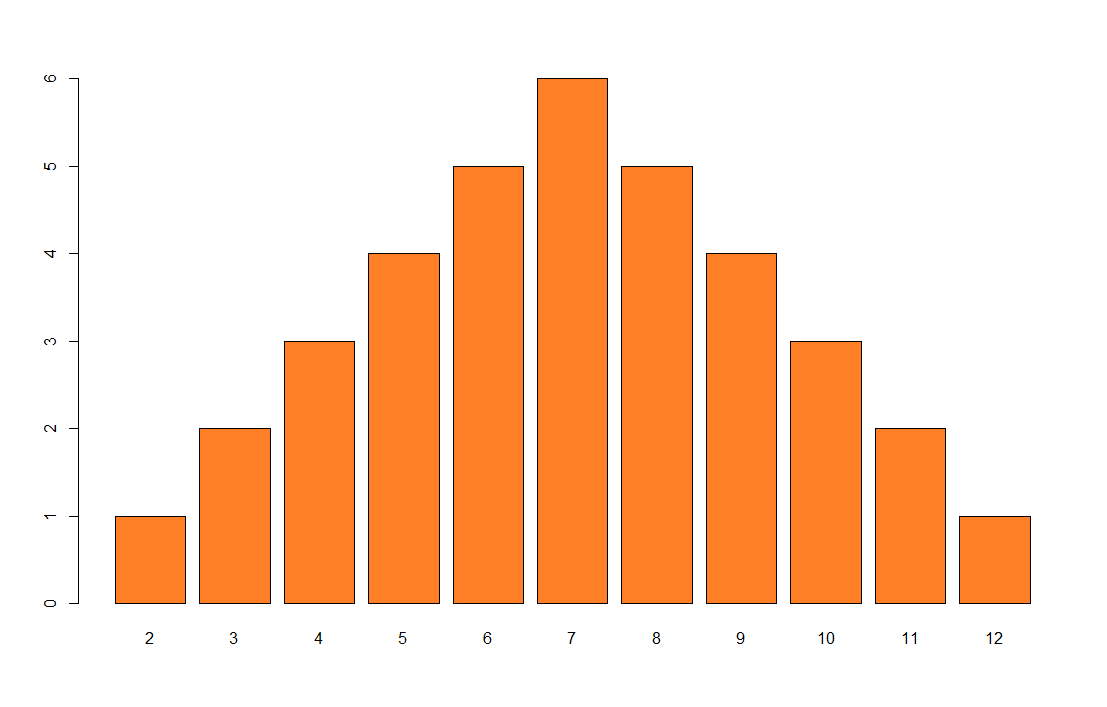
\includegraphics[width=12cm]{../fig/cap06-DistribucionOriginalVsMuestral-01.png}\\
(b)\\
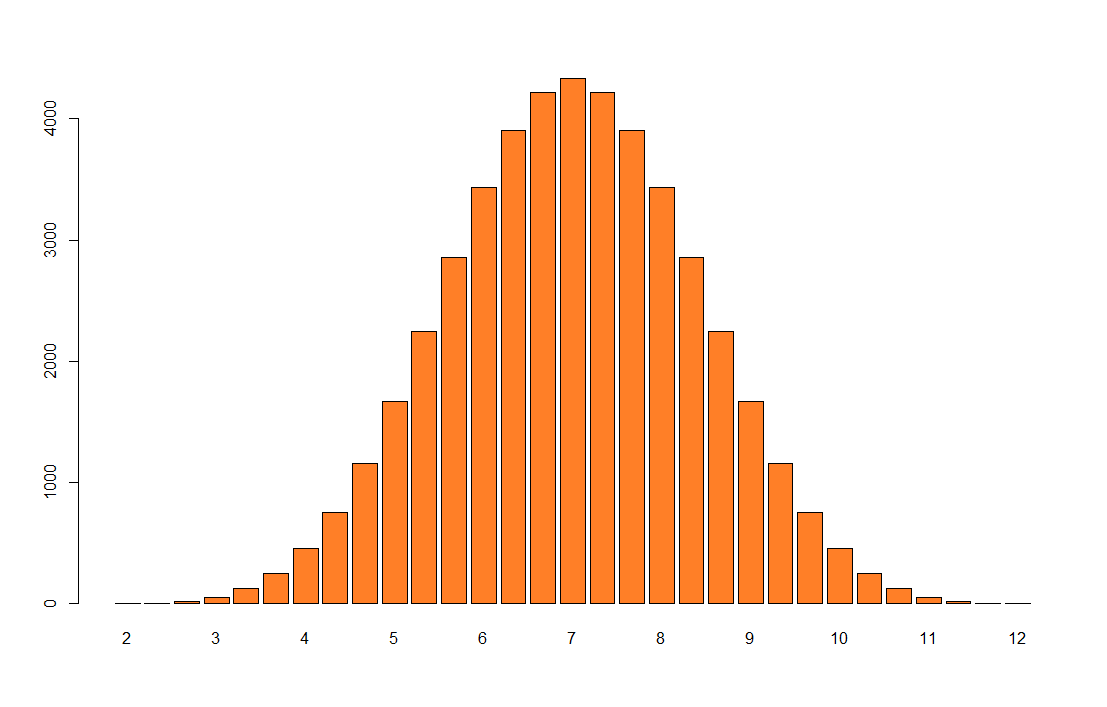
\includegraphics[width=12cm]{../fig/cap06-DistribucionOriginalVsMuestral-02.png}
\end{enColor}
\begin{bn}
(a)\\
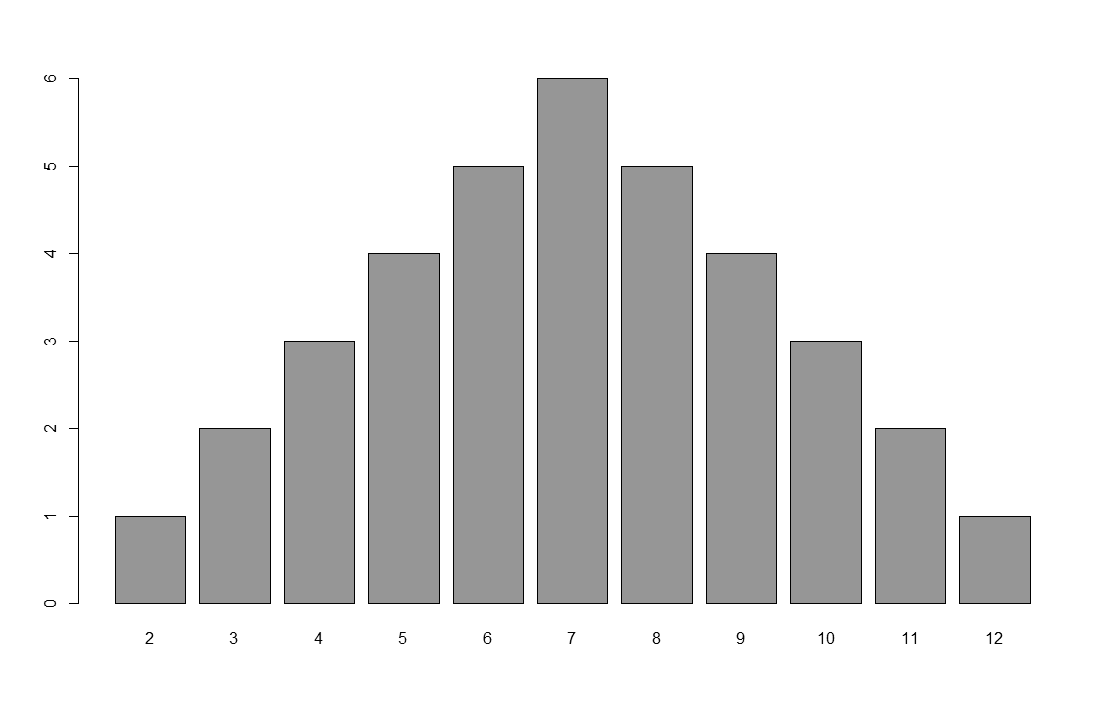
\includegraphics[width=12cm]{../fig/cap06-DistribucionOriginalVsMuestral-01-bn.png}\\
(b)\\
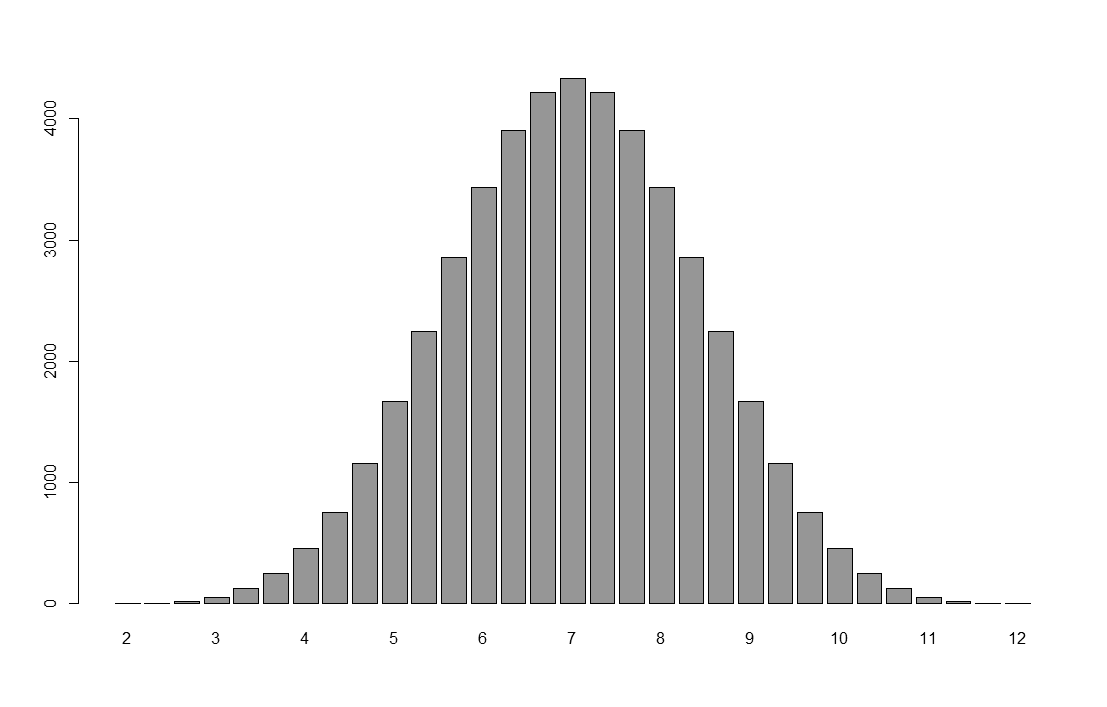
\includegraphics[width=12cm]{../fig/cap06-DistribucionOriginalVsMuestral-02-bn.png}
\end{bn}
\caption{(a) Distribución de la variable original $X$  y (b) de su media muestral $\bar X$.}
\label{cap06:fig:distribucionXvsMediasMuestrales}
\end{center}
\end{figure}

    ¿Sorprendidos con el resultado? Resulta que la forma de la distribución de la media muestral $\bar X$ es distinta. No tiene forma de v invertida, sino de campana. De hecho, es posible que nos haga pensar en la distribución normal... pero no adelantemos acontecimientos. Antes de eso, vamos a tratar de responder a las preguntas que hemos dejado en el aire, sobre la media y desviación típica de $\bar X$. La Figura \ref{cap06:fig:distribucionXvsMediasMuestrales} parece indicar que la media de $\bar X$ es $7$, la misma que la de $X$. Y en efecto, así es siempre, sea cual sea la variable aleatoria $X$:
        \[\mu_{\bar X}=\mu_X.\]
    Sabemos que es fácil perderse con la notación, entre $X$ y $\bar X$, así que vamos a pararnos un momento a tratar de aclarar el significado del símbolo $\mu_{\bar X}$. Es {\em la media de las medias muestrales}, calculada usando las 46656 medias muestrales que podemos obtener. Si no usamos la tabla de frecuencia, sino los valores directamente, $\mu_{\bar X}$ se calcularía así:
        \[\mu_{\bar X}=
        \dfrac{\overbrace{\bar X(d_1,d_1,d_1)+\bar X(d_1,d_1,d_2)+\cdots+\bar X(d_2,d_{15},d_{23})+\cdots+\bar X(d_{36},d_{36},d_{36})}^{\mbox{\small(Hay 46656 sumandos en el numerador)}} }{46656}=
        \]
        \[=\dfrac{\left(\dfrac{2+2+2}{3}\right)+\left(\dfrac{2+2+3}{3}\right)+\cdots+\left(\dfrac{3+6+9}{3}\right)+\cdots+\left(\dfrac{12+12+12}{3}\right)}{46656}.\]
    Y otra forma de calcularla es a partir de los valores agrupados de la Tabla \ref{cap06:tabla:TablaFrecuenciasMediasMuestrales}. En el Tutorial06 tendremos ocasión de calcular esta media de las dos formas, y confirmaremos que coincide con $\mu_X$.

    Una vez calculada la media $\mu_{\bar X}$ de $\bar X$, podemos calcular su desviación típica $\sigma_{\bar X}$. %Pero antes de ponernos manos a la obra queremos evitar desde el principio una posible confusión que a veces aparece, sobre el significado de $\sigma_{\bar X}$.
    De nuevo, mirando la Figura \ref{cap06:fig:distribucionXvsMediasMuestrales}, parece ser que la dispersión de $\bar X$ es menor que la de $X$: la campana es más {\em ``esbelta''} que la $v$ invertida. Este es, a nuestro juicio, el resultado que más puede sorprender al lector.  El proceso de muestreo no sólo no ha dispersado los valores, sino que los ha hecho agruparse más en torno a la media. Vamos a confirmar esto calculando $\sigma_{\bar X}$ y comparándola con $\sigma_X$. Nos espera otra sorpresa.

    El valor $\sigma_{\bar X}$ del que vamos a hablar es la raíz cuadrada de:
    {\small
        \begin{equation}\label{cap06:ecu:VarianzaDeMediasMuestrales}
        \begin{array}{c}
        \sigma^2_{\bar X}=
        \dfrac{\overbrace{
        (\bar X(d_1,d_1,d_1)\colorbox{lightgrey}{$-\mu_{\bar X}$})^{\colorbox{lightgrey}{2}}+
        (\bar X(d_1,d_1,d_2)\colorbox{lightgrey}{$-\mu_{\bar X}$})^{\colorbox{lightgrey}{2}}+
        \cdots+
        (\bar X(d_{36},d_{36},d_{36})\colorbox{lightgrey}{$-\mu_{\bar X}$})^{\colorbox{lightgrey}{2}}
        }^{\mbox{\small(Otra vez 46656 sumandos en el numerador)}} }{46656}=
        \\[8mm]
        =\dfrac{\left(\dfrac{2+2+2}{3}\colorbox{lightgrey}{-7}\right)^{\colorbox{lightgrey}{2}}
        +\left(\dfrac{2+2+3}{3}\colorbox{lightgrey}{-7}\right)^{\colorbox{lightgrey}{2}}+
        \cdots+\left(\dfrac{12+12+12}{3}\colorbox{lightgrey}{-7}\right)^{\colorbox{lightgrey}{2}}}{46656}.
        \end{array}
        \end{equation}
        }
        En particular, {\bf no estamos hablando} de la cuasivarianza muestral, que se puede calcular para cada muestra individual. Para intentar dejarlo más claro, igual que el cálculo
        \[\dfrac{3+6+9}{3}=\dfrac{18}{3}=6\]
        nos llevó a decir que
        \[\bar X(d_1,d_{15},d_{23})=6,\]
        ahora podríamos calcular la cuasivarianza muestral:
        \[\dfrac{(3-6)^2+(6-6)^2+(9-6)^2}{3},\]
        y tendríamos 46656 de estas cuasivarianzas. Pero, insistimos, {\sf no es eso lo que estamos haciendo}, sino lo que indica la Ecuación \ref{cap06:ecu:VarianzaDeMediasMuestrales}, cuyo resultado es un único valor. Volveremos sobre esas varianzas de cada una de las muestras en un capítulo posterior.

        Al completar él cálculo de $\sigma_{\bar X}$ en la Ecuación \ref{cap06:ecu:VarianzaDeMediasMuestrales} se obtiene:
        \[\sigma_{\bar X}=1.394\]
        qué es bastante más pequeño que el valor (que ya conocíamos) de $\sigma_X=\frac{\sqrt{35}}{6}\approx 2.415$. De hecho, Si dividimos ambas desviaciones típicas, y elevamos el resultado al cuadrado, tenemos
        \[\left(\dfrac{\sigma_{\bar X}}{\sigma_X}\right)^2=3.\]
        No es {\em aproximadamente} 3; es {\sf exactamente} $3$. ¿De dónde sale este $3$? Es fácil intuir que ese número es el tamaño de la muestra: estamos tomando muestras de tres valores de la variable original $X$. \qed

\end{ejemplo}

Enseguida vamos a dar una justificación más teórica de los resultados que hemos
observado en este ejemplo tan largo. Pero ahora queremos detenernos en otro
tipo de explicación, más informal, pero quizá más intuitiva. Lo que sucede es
que, en cada muestra de tres valores, es más probable que haya dos cercanos a
la media, que pueden compensar un posible valor alejado de la media. Y la
combinatoria se encarga de asegurar que haya muchas, muchas más de estas
muestras ``normales'', en comparación con el número de muestras ``raras'', como
$m_1=\left((1,1),(1,1),(1,1)\right)$. Las frecuencias de la Tabla
\ref{cap06:tabla:TablaFrecuenciasMediasMuestrales} confirman esa superioridad
numérica de las muestras cercanas a la media. Es decir, que el proceso de
muestreo matiza o lima las diferencias entre los distintos valores que toma la
variable, empujándolos a todos hacia la media. Y si el fenómeno se observa
incluso para un valor tan modesto como $n=3$ ¿qué pasará cuando, en otros
ejemplos, se tomen muestras de, por ejemplo, $n=10000$?

Para profundizar en nuestra comprensión de este fenómeno, y entender la
relación entre $\sigma_{\bar X}$ y $\sigma_X$, necesitamos un poco de
formalismo. Afortunadamente, tenemos todo lo que necesitamos, y el razonamiento
es bastante sencillo.

La media muestral de tamaño $n$, es la suma de $n$ variables aleatorias {\sf
independientes}, que corresponden a cada uno de los $n$ valores de la variable
inicial $X$ que se han seleccionado para la muestra:
    \[\bar X=\dfrac{X_1+X_2+\cdots+X_n}{n}=\dfrac{X_1}{n}+\dfrac{X_2}{n}+\cdots+\dfrac{X_n}{n}\]
Y las variables $X_i$ son copias de $X$, así que todas tienen media $\mu_X$ y
desviación típica $\sigma_X$. Por lo tanto, en primer lugar, como habíamos
anticipado:
    \begin{equation}\label{cap06:ecu:EsperanzaMediaMuestral}
    \mu_{\bar X}=E(\bar X)=\dfrac{E(X_1)+E(X_2)+\cdots+E(X_n)}{n}=\dfrac{n\cdot \mu_X}{n}=\mu_X.
    \end{equation}
Y en segundo lugar, para la desviación típica, {\sf puesto que $X_1,\ldots,X_n$
son independientes}:
    \[\sigma^2_{\bar X}=\operatorname{Var}(\bar X)=\operatorname{Var}\left(\dfrac{X_1}{n}\right)+\operatorname{Var}\left(\dfrac{X_2}{n}\right)+\cdots+\operatorname{Var}\left(\dfrac{X_n}{n}\right)=
    n\cdot\dfrac{\operatorname{Var}(X)}{n^2}=\dfrac{\sigma^2_X}{n}.\]
Esta última fórmula explica de donde proviene el $3$ que hemos encontrado al
final del Ejemplo \ref{cap06:ejem:DistribucionMediaMuestral}, al comparar
$\sigma_{\bar X}$ con $\sigma_X$. Vamos a hacer oficiales las conclusiones que
hemos obtenido:
    \begin{center}
    \fcolorbox{black}{Gris025}{
    \begin{minipage}{12.5cm}
        \begin{center}
        %%%%%%%%%%%%%%%%%%%%%%%%%%%%%%%%%%%%%%%
        {\bf  La media muestral $\bar X$ y su distribución.}\\
        \end{center}
        \index{distribución de la media muestral}
        \index{media muestral, distribución}
       %%%%%%%%%%%%%%%%%%%%%%%%%%%%%%%%%%%%%%%
        Sea $X$ una variable aleatoria cualquiera, con media $\mu_X$ y desviación típica $\sigma_X$.
       \begin{enumerate}
       \item Una \index{muestra aleatoria simple}{\sf muestra aleatoria
           simple de tamaño $n$} de $X$ es una lista $(X_1,X_2,\ldots,X_n)$
           de $n$ copias {\sf independientes} de la variable $X$. Ver más detalles en la Sección \ref{cap06:sec:MuestraAleatoriaSimpleFuncionVerosimilitud} (pág. \pageref{cap06:sec:MuestraAleatoriaSimpleFuncionVerosimilitud})
       \item La \index{media muestral}{\sf media muestral} de $X$ es la
           variable aleatoria
       \begin{equation}
       \label{cap06:ecu:MediaMuestral}
        \bar X=\dfrac{X_1+\cdots+X_n}{n}
        \end{equation}
       \item Al considerar las muestras aleatorias simples, de tamaño $n$, de
           una variable aleatoria $X$ cualquiera, se obtienen estos
           resultados para la media y la desviación típica de la media
           muestral:
        \[\mu_{\bar X}=\mu_X,\qquad \sigma_{\bar X}=\dfrac{\sigma_X}{\sqrt{n}}.\]
        El valor $\sigma_{\bar X}$  tambi\'en se llama \index{error
        muestral}{\sf error muestral}.
       \end{enumerate}
        %%%%%%%%%%%%%%%%%%%%%%%%%%%%%%%%%%%%%%%
    \end{minipage}}
    \end{center}

De nuevo le pedimos al lector que haga un esfuerzo especial para entender estos
resultados, que lea otros textos, busque ejemplos, etc. El fenómeno que hemos
tratado de poner de manifiesto es que el proceso de muestreo aleatorio hace
una especie de ```truco de magia'' con la media, de manera que la media muestral está
menos dispersa que la variable original. Y el fenómeno es tanto más acusado
cuanto mayor sea la muestra, {\bf sin que importe el tamaño de la población.}
Hay que saborear por un momento estas palabras, porque apuntan a uno de los
motores que realmente mueven la Estadística, y una de las razones fundamentales
que la convierten en una herramienta valiosa. A menudo, los no versados en
Estadística se sorprenden de que un Estadístico pretenda poder decir algo
sobre, por ejemplo, el resultado de unas elecciones, cuando sólo ha preguntado
su intención de voto a, digamos, diez mil personas, sobre un censo de cuarenta
millones. Lo que se está dejando de ver, en un caso como este, es que si la
muestra fuera realmente aleatoria, la dispersión muestral, con $n=10000$, sería
cien veces menor que la de la población completa. Simplificando mucho, al
estadístico le resulta cien veces más fácil acertar de lo que podría pensarse
en un principio. Como hemos dicho, estamos simplificando mucho las cosas, y en
particular, ese ideal de la muestra verdaderamente aleatoria está muy lejos de
lo que, en realidad, podemos o queremos hacer. En este curso no vamos a tener
ocasión de entrar en el tema de las distintas formas de muestreo, y del
problema más general del Diseño Experimental. Pero haremos algunos comentarios
al presentar la Bibliografía, en la página
\pageref{apendice:comentarioBibliografia}.


\subsection{El Teorema Central del Límite, otra vez.}
\label{cap06:subsec:teoremaCentralLimiteSegundaVersion}

En el Capítulo \ref{cap:TeoremaCentralLimite} vimos que De Moivre había
descubierto que, cuando $n$ se hace más y más grande, una variable de tipo
binomial $B(n,p)$ se parece cada vez más a una variable de tipo normal $N(\mu,
\sigma)$, para los valores adecuados $\mu=n p$ y $\sigma=\sqrt{npq}$. Ese fue
nuestro primer encuentro con el Teorema Central del Límite (pág.
\pageref{cap05:teo:TCL}). Ahora queremos volver sobre una observación que hemos
hecho de pasada en el Ejemplo \ref{cap06:ejem:DistribucionMediaMuestral}, al
hilo de la Figura \ref{cap06:fig:distribucionXvsMediasMuestrales} (pág.
\pageref{cap06:fig:distribucionXvsMediasMuestrales}), en la que comparábamos la
forma de la distribución de $X$ con la de su media muestral $\bar X$. En ese
ejemplo hemos empezado con una variable aleatoria que, desde luego, no es
binomial ({\em no estamos  midiendo éxitos de ningún tipo}). Y sin embargo,
cuando se observa la parte (b) de la Figura
\ref{cap06:fig:distribucionXvsMediasMuestrales}, parece evidente que la
distribución de la media muestral $\bar X$ se parece a la normal. {!`}Y aquí ni
siquiera hemos usado un $n$ muy grande, sólo estamos tomando $n=3$! Este
fenómeno es una nueva manifestación del Teorema Central del Límite, del que
ahora vamos a ver una segunda versión.

    \begin{center}
    \fcolorbox{black}{Gris025}{
    \begin{minipage}{12.5cm}
        \begin{center}
        %%%%%%%%%%%%%%%%%%%%%%%%%%%%%%%%%%%%%%%
        {\bf  Teorema central del l\'imite, segunda versi\'on.}\\
        \end{center}
        \index{distribución de la media muestral}
        \index{media muestral, distribución}
        \index{teorema Central del límite, segunda versión}
        \label{cap06:teo:TCLsegundaVersion}
       %%%%%%%%%%%%%%%%%%%%%%%%%%%%%%%%%%%%%%%
       Sea $X$ una variable aleatoria cualquiera, con media $\mu_X$ y desviación típica $\sigma_X$.
       \begin{enumerate}
       \item  {\sf Sea cual sea la forma de la distribución de $X$}, si se
           toman muestras aleatorias simples de $X$, de tamaño $n$, entonces
           cuando $n$ se hace cada vez más grande la distribución de la media
           muestral $\bar X$ se aproxima cada vez más a la normal
            \[N\left(\mu_X,\dfrac{\sigma_X}{\sqrt{n}}\right).\]
           En particular, para $n$ suficientemente grande (usaremos $n>30$),
           tenemos
            \[P(a\leq \bar X\leq b)\approx P\left(\dfrac{a-\mu_X}{\dfrac{\sigma_X}{\sqrt{n}}}\leq Z\leq \dfrac{b-\mu_X}{\dfrac{\sigma_X}{\sqrt{n}}}\right),\]
          siendo $Z$ de tipo  normal $N(0,1)$.
       \item Si además sabemos que la variable original $X$ es de tipo normal
           $N(\mu_X,\sigma_X)$, entonces, {\sf independientemente del tamaño
           $n$ de la muestra}, la media muestral también es normal, del mismo
           tipo
            \[N\left(\mu_X,\dfrac{\sigma_X}{\sqrt{n}}\right).\]
       \end{enumerate}
        %%%%%%%%%%%%%%%%%%%%%%%%%%%%%%%%%%%%%%%
    \end{minipage}}
    \end{center}

%    \begin{center}
%       \fbox{\colorbox{Gris025}{\begin{minipage}{14cm}
%       \begin{center}
%%       \vspace{2mm}
%       {\bf Teorema central del l\'imite, segunda versi\'on: }
%       %TEOREMA CENTRAL DEL LÍMITE, SEGUNDA VERSIÓN
%       \end{center}
%       Sea $X$ una variable aleatoria cualquiera, con media $\mu$ y desviación típica $\sigma$.
%       \begin{enumerate}
%       \item  {\sf Sea cual sea la forma de la distribución de $X$}, si se toman muestras de $X$ de tamaño $n$, entonces cuando $n$ se hace cada vez más grande la distribución de la media muestral
%          $\bar X$ se aproxima cada vez más a la normal $N\left(\mu_X,\dfrac{\sigma_X}{\sqrt{n}}\right)$. En particular, para $n$ grande tenemos
%          \[P(a\leq \bar X\leq b)\approx P\left(\dfrac{a-\mu_X}{\dfrac{\sigma_X}{\sqrt{n}}}\leq Z\leq \dfrac{b-\mu_X}{\dfrac{\sigma_X}{\sqrt{n}}}\right)\]
%          siendo $Z$ de tipo  normal $N(0,1)$.
%       \item Si además sabemos que la variable original es de tipo normal $N(\mu_X,\sigma_X)$, entonces, {\sf independientemente del tamaño $n$ de la muestra}, la media muestral también es normal, de tipo  $N\left(\mu_X,\dfrac{\sigma_X}{\sqrt{n}}\right)$.
%       \end{enumerate}
%       \end{minipage}
%       }}
%       \end{center}%\\[3mm]
El resultado es tan importante, que vamos a repetirlo con otras palabras. En
resumidas cuentas:
\begin{itemize}
  \item Para muestras suficientemente grandes, las medias muestrales de todas
      las variables, {!`}sea cual sea el tipo de variable!, se comportan como
      variables normales.
  \item Pero además, si hemos empezado con una variable normal, entonces el
      tamaño de la muestra es irrelevante.
\end{itemize}
Esta última parte es muy importante, cuando se tiene en cuenta la primera
versión del Teorema Central del Límite. Aquella primera versión nos hizo pensar
que las variables normales o muy aproximadamente normales debían ser frecuentes
en la naturaleza. Y esta versión nos asegura que el comportamiento en el
muestreo de esas variables normales es especialmente bueno. Combinados, los dos
resultados nos dicen que la distribución normal debe considerarse como una de
las leyes fundamentales de la naturaleza.

Por supuesto, el Teorema no cubre todas las situaciones posibles. Para empezar,
tenemos que precisar lo que sucede  cuando la variable $X$ no es normal. ¿De
que tamaño tiene que ser la muestra para que la aproximación de $\bar X$
mediante una normal sea válida? Volveremos sobre esto antes del final del
capítulo.
%Pero ahora, sobre todo, queremos dejar claro que el Teorema se refiere
%
%Esas son las buenas noticias. Las malas noticias son que, si no podemos suponer que la variable $X$ sea normal, entonces, en general, no sabremos de que tamaño tiene que ser la muestra para que la aproximación normal sea válida. Puede ocurrir que se necesite una muestra muy grande. Y en muchos caso, no tendremos muestras tan grandes. \pendiente{Volveremos sobre este punto más adelante.}

Con esta segunda versión del Teorema Central del Límite hemos llegado a un hito
importante en el curso. Hasta aquí, en los últimos capítulos,  todo lo que
hemos hecho es Teoría de la Probabilidad. Pero ahora estamos listos para
empezar a hace Inferencia, que es el núcleo central de la Estadística
propiamente dicha. Vamos a empezar a hacer lo que venimos anunciando desde el
principio del curso. En la próxima sección vamos a utilizar las muestras para
tratar de obtener información sobre la población.

%
%
%En la próxima Además, hay una dificultad añadida. Para usar este resultado, necesitaríamos conocer la desviación típica de la población. Dejamos pendiente para la próxima sección este problema, junto con el problema de cómo obtener las muestras que mencionábamos al principio.

%\section*{\fbox{\colorbox{Gris025}{{Sesión 17. Inferencia estadística.}}}}
%
%\subsection*{\fbox{\colorbox{Gris025}{{Intervalos de confianza para la media.}}}}
%\subsection*{Fecha: Viernes, 11/11/2011, 14h.}
%
%\noindent{\bf Atención:
%\begin{enumerate}
%\item Este fichero pdf lleva adjuntos los ficheros de datos necesarios.
%\end{enumerate}
%}
%
%%\subsection*{\fbox{1. Ejemplos preliminares }}
%\setcounter{tocdepth}{1}
%%\tableofcontents

\section{Intervalos de confianza para la media en poblaciones normales.}
\label{cap06:sec:IntervaloConfianzaMediaPoblacionNormal}

Para empezar a hacer Inferencia, nuestro primer objetivo es usar el valor de
$\bar X$ obtenido en una muestra, para  poder llegar a una predicción sobre
$\mu_X$, la media de la población. Estamos suponiendo que la variable $X$ se distribuye en la población como una normal $N(\mu, \sigma)$. Tenemos razones teóricas para creer que esto puede funcionar, gracias al Teorema Central del Límite. El tipo de predicciones que vamos a tratar de obtener tienen la forma de frases como esta:
   \begin{equation}\label{cap06:ecu:IntervaloConfianzaVersionInformal}
   \mbox{\sf Hay una probabilidad del 90\% de que $\mu_X$ esté dentro del intervalo $(a,b)$.}
   \end{equation}
Como puede verse:
\begin{itemize}
  \item La predicción se refiere a un intervalo $(a,b)$ de valores. No
      decimos {\sf cuál es} el valor de $\mu_X$, sino que decimos algo sobre
      {\sf dónde está}. La predicción, por tanto, siempre va a incorporar un
      cierto margen de error.
  \item La predicción se hace en términos de probabilidad. Tampoco estamos
      afirmando que el valor de $\mu_X$ está, con absoluta seguridad, dentro
      del intervalo $(a,b)$. Hay un margen de incertidumbre, que se
      refleja en esa probabilidad del 90\%.
\end{itemize}
Estas dos características, el margen de error y el margen de incertidumbre,
acompañan siempre a las predicciones estadísticas. Desde el punto de vista del
método científico, representan un gran avance, puesto que hacen cuantificable,
medible y fácil de comunicar, la fiabilidad de nuestras afirmaciones. Son un
ingrediente básico para alcanzar los principios de objetividad y honestidad
intelectual, que deben guiar en todo momento el trabajo científico. No son una
debilidad, sino una fortaleza del método científico. {!`}Y, al fin y al cabo, son
inevitables! Sabemos que la previsión se basa en el muestreo, e incluso en el
mejor de los casos, en un muestreo aleatorio simple como el del Ejemplo
\ref{cap06:ejem:DistribucionMediaMuestral}, siempre hay una fracción de
muestras ``raras'', que se alejan de la media mucho más que el resto. Siempre
tenemos que contemplar la posibilidad de que {\em nuestra muestra}, la que nos
ha tocado en el estudio o experimento que hayamos hecho, sea una de esas
muestras ``raras''. Y lo único que, honestamente, podemos hacer es tratar de
medir de la mejor manera posible la probabilidad de acertar en nuestras
predicciones.

Hablando de probabilidades, tenemos que aclarar lo que queremos decir cuando,
en una predicción como \ref{cap06:ecu:IntervaloConfianzaVersionInformal},
decimos que hay una probabilidad del 90\% de que $\mu_X$ esté en $(a,b)$.
Simplificando el problema, en ese 90\%, ¿cuáles son los casos posibles, y
cuáles los favorables? Para responder vamos a considerar el espacio muestral
formado por las muestras de tamaño $n$ de la variable $X$, con muestreo
aleatorio simple, de manera que todas las muestras de tamaño $n$ son
equiprobables. Y entonces podemos pensar que el 90\% de
\ref{cap06:ecu:IntervaloConfianzaVersionInformal} significa que la afirmación
\[\mu_X\mbox{ está en el intervalo }(a,b)\]
es cierta para el 90\% de las muestras de tamaño $n$. Todavía lo podemos
escribir de otra manera, usando el lenguaje de la probabilidad:
\begin{equation}\label{cap06:ecu:IntervaloConfianzaLenguajeProbabilidad}
P\left(a<\mu_X<b\right)=0.9
\end{equation}
Luego volveremos sobre esto, y sobre otras muchas preguntas que el lector se
puede estar haciendo. Pero primero queremos avanzar un poco más, empezando a
explicar cómo se calculan estos intervalos $(a,b)$, para llegar lo antes
posible a trabajar sobre ejemplos concretos. Aún nos queda bastante camino por
recorrer, pero vamos a intentar mantener un cierto equilibrio mientras
avanzamos. Son los detalles técnicos los que nos mueven, pero no queremos que
esos mismos detalles nos hagan olvidar el objetivo hacia el que nos movemos.

Un poco de terminología: el intervalo $(a,b)$ será un {\sf intervalo de
confianza}\index{intervalo de confianza, media en poblaciones normales} para
$\mu_X$, y el porcentaje del $90\%$ es el {\sf nivel de confianza}\index{nivel
de confianza} de ese intervalo. ¿Cómo se construyen estos intervalos?

La clave es el Teorema Central del Límite, y la información que nos proporciona
sobre la distribución de la media muestral $\bar X$. El teorema, tal como lo
hemos visto, tiene dos partes: la parte (a) habla sobre cualquier variable,
mientras que la parte (b) habla de variables normales. Para simplificar, vamos
a empezar con esta segunda, porque es la más fácil de la dos, ya que no depende
del tamaño de la muestra.

Estamos suponiendo, por tanto que $X$ es una variable aleatoria de tipo normal
$N(\mu_X,\sigma_X)$. Hemos obtenido una muestra aleatoria de $X$, de tamaño
$n$, que será una colección de valores
\[x_1,x_2,\ldots,x_k,\]
y queremos usar estos valores para construir un intervalo de confianza para
$\mu_X$. La muestra, desde luego, no es la población, así que no podemos usarla
para calcular $\mu_X$. En su lugar, como hemos visto, calculamos la media
muestral
\[\bar X=\dfrac{x_1+x_2+\cdots+x_n}{n}.\]
El Teorema Central del Límite (parte (b)), nos dice que $\bar X$ es una
variable normal, de tipo  \[N\left(\mu_X,\dfrac{\sigma_X}{\sqrt{n}}\right).\] Y
por tanto, si aplicamos la tipificación (recuerda la Sección \ref{cap05:subsec:DistribucionNormalEstandarTipificacion}):
    \begin{equation}\label{cap06:ecu:TipificacionMediaMuestral}
    Z=\dfrac{\bar X-\mu_X}{\dfrac{\sigma_X}{\sqrt{n}}},
    \end{equation}
obtendremos una variable $Z$, de tipo normal estándar $N(0,1)$. ¿Para qué nos
sirve tipificar? Lo bueno de trabajar con una normal estándar $Z$ es que es una
variable de la que sabemos mucho. En particular, en el siguiente apartado
\ref{cap06:subsec:valoresCriticosZ}
 de este capítulo, y en el Tutorial06 aprenderemos a calcular un valor $K$ tal que (ver Figura \ref{cap06:fig:ProblemaInversoZIntervalo90}, pág. \pageref{cap06:fig:ProblemaInversoZIntervalo90})
\begin{equation}\label{cap06:ecu:ValorKIntervalo90EnZ}
P(-K< Z <K)=0.9
\end{equation}
Este es uno de esos momentos en que tenemos que buscar el equilibrio entre los
detalles técnicos, y la idea que vamos persiguiendo. En el próximo apartado
están los detalles técnicos del cálculo de $K$. Pero antes de embarcarnos en
eso, queremos hacer ver para qué nos van a servir. Si comparamos la Ecuación
\ref{cap06:ecu:ValorKIntervalo90EnZ} con la forma probabilista del intervalo de
confianza, en la Ecuación
\ref{cap06:ecu:IntervaloConfianzaLenguajeProbabilidad}, vemos que las dos son
afirmaciones parecidas. Y de hecho, vamos a hacerlas aún más parecidas.
Sustituyendo la Ecuación \ref{cap06:ecu:TipificacionMediaMuestral} de
tipificación, en la \ref{cap06:ecu:ValorKIntervalo90EnZ} tenemos:
\[
P\left(-K< \dfrac{\bar X-\mu_X}{\dfrac{\sigma_X}{\sqrt{n}}} <K\right)=0.9
\]
Y lo bueno de esta expresión es que nos va a permitir despejar $\mu_X$ para
llegar a una ecuación como \ref{cap06:ecu:ValorKIntervalo90EnZ}, que es nuestro
objetivo. Lo repetiremos cuando hayamos calculado $K$, pero ahí va un adelanto.
De las desigualdades que hay dentro del paréntesis, multiplicando todos los
términos por $\dfrac{\sigma_X}{\sqrt{n}}$ se obtiene:
    \[
    -K\dfrac{\sigma_X}{\sqrt{n}}< \bar X-\mu_X<K\dfrac{\sigma_X}{\sqrt{n}}.
    \]
Y de aquí, con un poco de cuidado con los signos y las desigualdades, llegamos
a:
    \[
    \bar X-K\dfrac{\sigma_X}{\sqrt{n}}< \mu_X<\bar X+K\dfrac{\sigma_X}{\sqrt{n}}.
    \]
Por lo tanto, una vez que encontremos $K$, podemos asegurar que se cumple:
    \[
    P\left(\underbrace{\bar X-K\dfrac{\sigma_X}{\sqrt{n}}}_a< \mu_X<
    \underbrace{\bar X+K\dfrac{\sigma_X}{\sqrt{n}}}_b\right)=0.9,
    \]
y esta es una ecuación de la forma
\[P\left(a<\mu_X<b\right)=0.9\]
Es decir, es una fórmula para el intervalo de confianza. Como vemos, todo pasa
por el cálculo de ese valor $K$, y eso es lo que vamos a hacer a continuación.

%cap06:ecu:IntervaloConfianzaLenguajeProbabilidad
%
%Como hemos dicho, al pensar en este tipo de predicciones mediante intervalos, hay que tener en cuenta tanto el nivel de confianza como la anchura del intervalo. Pero esas dos cantidades no son independientes. En general, nosotros elegiremos uno de los dos como objetivo, y obtendremos el otro mediante un cálculo.
%
%Los niveles de confianza más frecuentes son $90\%$, $95\%$ y $99\%$. Hablando en general, el nivel de confianza está relacionado con la anchura del intervalo (cuánto mayor sea el margen de error, más segura es la predicción. {!`}Pero también es menos precisa!) y con el tamaño de la muestra (cuántos más elementos incluya la muestra, mayor será la precisión de la predicción). Es decir, {\em conseguir un intervalo muy pequeño, con una probabilidad muy alta, requiere más trabajo (por ejemplo, en forma de muestras más grandes)}.
%
%
%
%
%
%
%
%
%Nuestro objetivo es, como decíamos al principio de la sección, es usar el valor de $\bar X$ obtenido en una muestra, para  poder llegar a una predicción sobre $\mu_X$. El tipo de predicciones que vamos a hacer sigue el esquema de esta frase:
%       \begin{center}
%       {\sf Hay una probabilidad del 90\% de que el valor de $\mu_X$ esté dentro del intervalo $(a,b)$.}
%       \end{center}
%El intervalo $(a,b)$ será un {\sf intervalo de confianza} para $\mu_X$, y el porcentaje del $90\%$ es el {\sf nivel de confianza} que deseamos. Los niveles de confianza más frecuentes son $90\%$, $95\%$ y $99\%$. Hablando en general, el nivel de confianza está relacionado con la anchura del intervalo (cuánto mayor sea el margen de error, más segura es la predicción. {!`}Pero también es menos precisa!) y con el tamaño de la muestra (cuántos más elementos incluya la muestra, mayor será la precisión de la predicción). Es decir, {\em conseguir un intervalo muy pequeño, con una probabilidad muy alta, requiere más trabajo (por ejemplo, en forma de muestras más grandes)}.
%
%¿Cómo se construyen estos intervalos? Vamos a empezar recordando el último resultado de la anterior sesión, que es una de las formas que adopta el Teorema Central del Límite:%\\[3mm]
%    \begin{center}
%       \fbox{\colorbox{Gris025}{\begin{minipage}{14cm}
%       \begin{center}
%%       \vspace{2mm}
%%       {\bf TEOREMA CENTRAL DEL LÍMITE, POBLACIÓN NORMAL}\\
%       {\bf Teorema central del l\'imite, poblaci\'on normal: }
%       \end{center}
%       Sea $X$ una variable aleatoria normal, de tipo $N(\mu_X,\sigma_X)$. Entonces, {\sf independientemente del tamaño $n$ de la muestra}, la media muestral $\bar X$ también es normal, de tipo  $N\left(\mu_X,\dfrac{\sigma_X}{\sqrt{n}}\right)$.\\ Y por tanto, si definimos (tipificamos):
%          \[Z=\dfrac{\bar X-\mu_X}{\dfrac{\sigma_X}{\sqrt{n}}},\]
%          la variable $Z$ es de tipo normal estándar $N(0,1)$.
%       \end{minipage}
%       }}
%       \end{center}%\\[3mm]
%       Y lo bueno de este resultado es que estamos muy bien preparados para responder a cualquier tipo de preguntas sobre la variable normal estándar $Z$. Antes de seguir con los intervalos de confianza, vamos a
%       detenernos para dejar claros estos detalles referentes a la normal.
%
%
\subsection{Valores críticos de la distribución normal estándar. Problemas de probabilidad directos e inversos.}
\label{cap06:subsec:valoresCriticosZ}

En este apartado nos vamos a concentrar en el caso, especialmente importante, de una variable $Z$ con distribución normal estándar $N(0,1)$. Sobre todo, queremos desarrollar el lenguaje que vamos a necesitar para describir nuestro trabajo, y para hablar de los problemas que se plantean. En los tutoriales aprenderemos a resolver esos problemas usando el ordenador.

Al trabajar con Z, vamos a distinguir dos tipos de preguntas. Y a su vez, cada
uno de esos dos tipos genéricos nos llevará a dos subtipos de preguntas
concretas. Empezamos con las preguntas más evidentes, que son las que vamos a llamar {\sf
problemas directos}\index{problemas directos, Z} de probabilidad. La
característica común a estos problemas es que los datos que tenemos son {\sf
valores} de $Z$, y lo que se quiere averiguar es una {\sf probabilidad}.

\begin{ejemplo}
\label{cap06:ejem:ProblemaDirectoProbabilidadZ}
Un ejemplo típico sería esta pregunta:
\begin{center}
{\em ``¿Cuánto vale la probabilidad $P(-2 < Z < 1.5)$?''}
\end{center}
Como puede verse, la respuesta que buscamos es una probabilidad. Y los datos
que aparecen, $-2$ y $1.5$ son valores de $Z$. Si pensamos en la función de
densidad de la variable normal $Z$, el problema se puede representar como en la
Figura \ref{cap06:fig:ValoresCriticos01}. En el Tutorial06 veremos que la probabilidad es aproximadamente igual a $0.9104$. \qed

\begin{figure}[h]
\begin{center}
\begin{enColor}
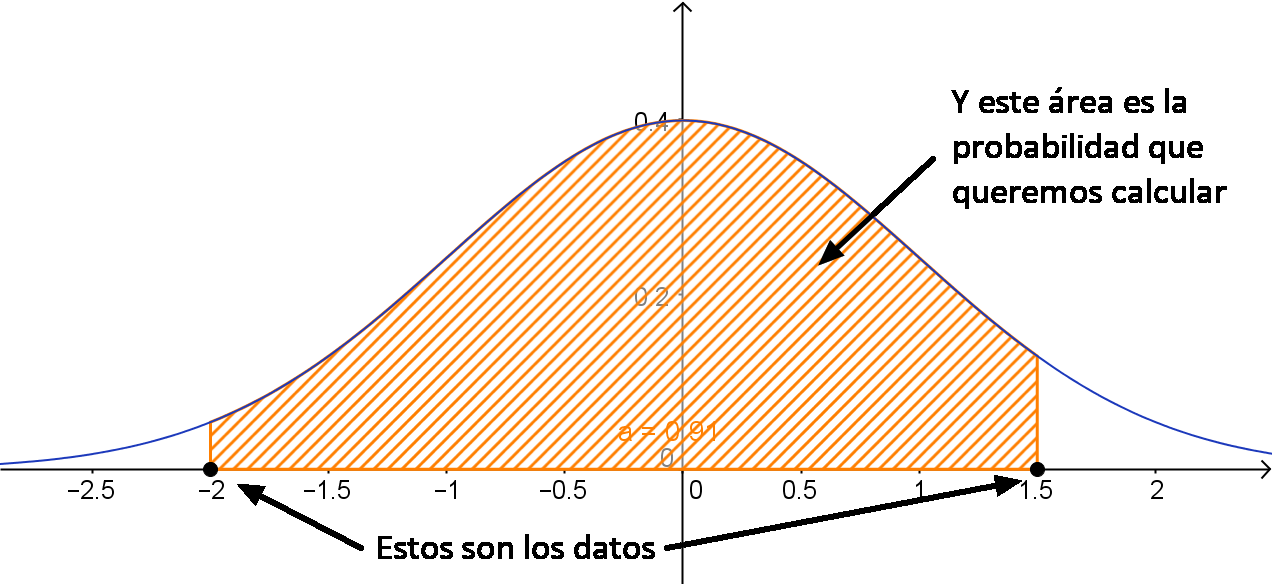
\includegraphics[width=11cm]{../fig/Cap06-ValoresCriticos01.png}
\end{enColor}
\begin{bn}
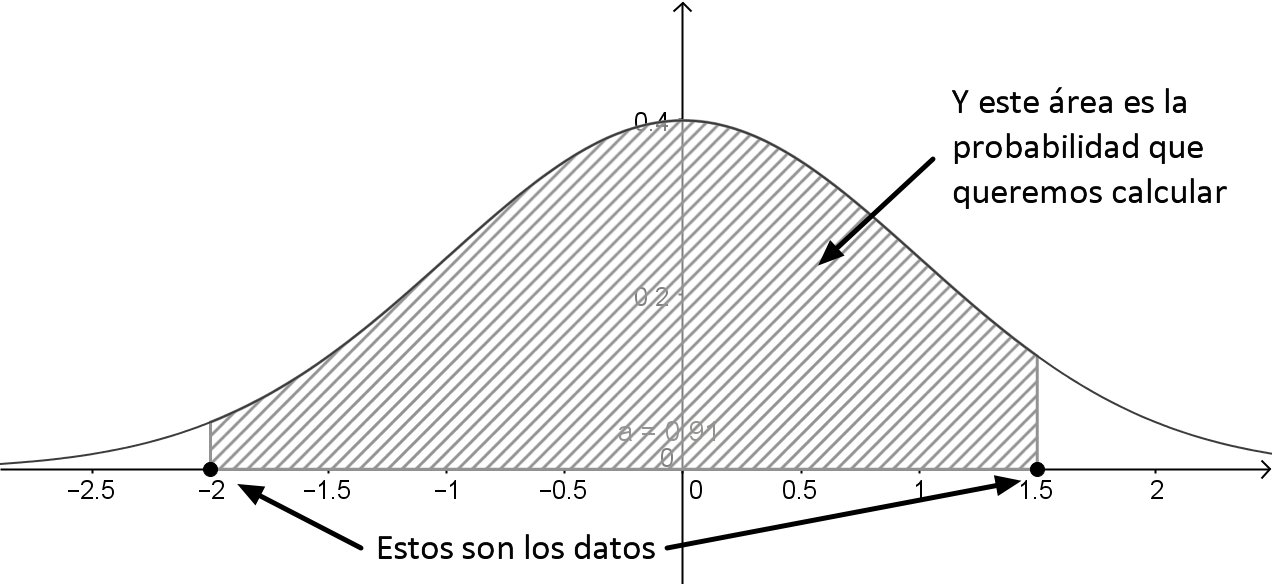
\includegraphics[width=11cm]{../fig/Cap06-ValoresCriticos01-bn.png}
\end{bn}
\caption{Un problema directo de probabilidad en $Z$.}
\label{cap06:fig:ValoresCriticos01}
\end{center}
\end{figure}
\end{ejemplo}

Dentro de los problemas directos, vamos a distinguir dos clases de preguntas.
\begin{itemize}
  \item Preguntas sobre la probabilidad de un {\sf intervalo acotado}, de la
      forma
  \[P(a<Z<b),\]
  donde $a$ y $b$ son dos números finitos, como en el ejemplo de la Figura
  \ref{cap06:fig:ValoresCriticos01}.
  \item Preguntas sobre la probabilidad de una {\sf cola} de la distribución
      normal. Es decir, preguntas de una de estas dos formas:
      \[
      \begin{cases}
      P(Z>a),\quad \mbox{(cola derecha).}\\[3mm]
      P(Z<a),\quad \mbox{(cola izda).}
      \end{cases}
      \]
\end{itemize}
Las preguntas sobre colas de la distribución $Z$ se ilustran en la Figura
\ref{cap06:fig:ProblemasColasZ}.

\begin{figure}[p]
\begin{center}
\begin{enColor}
\begin{tabular}{c}
(a1)\\
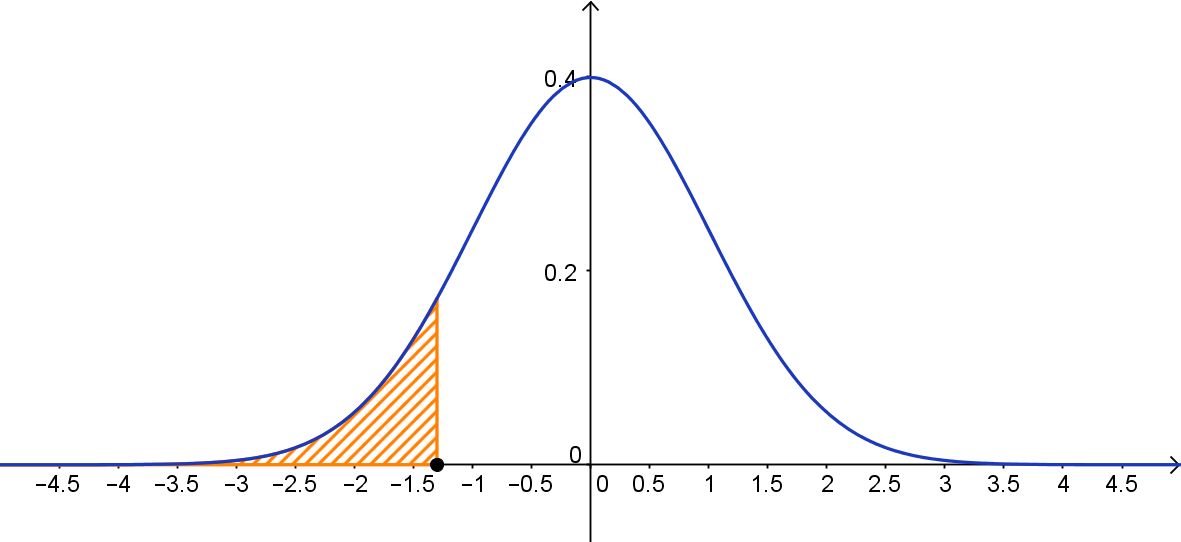
\includegraphics[width=9cm]{../fig/Cap06-ColaIzquierdaZ-01.png}\\
(a2)\\
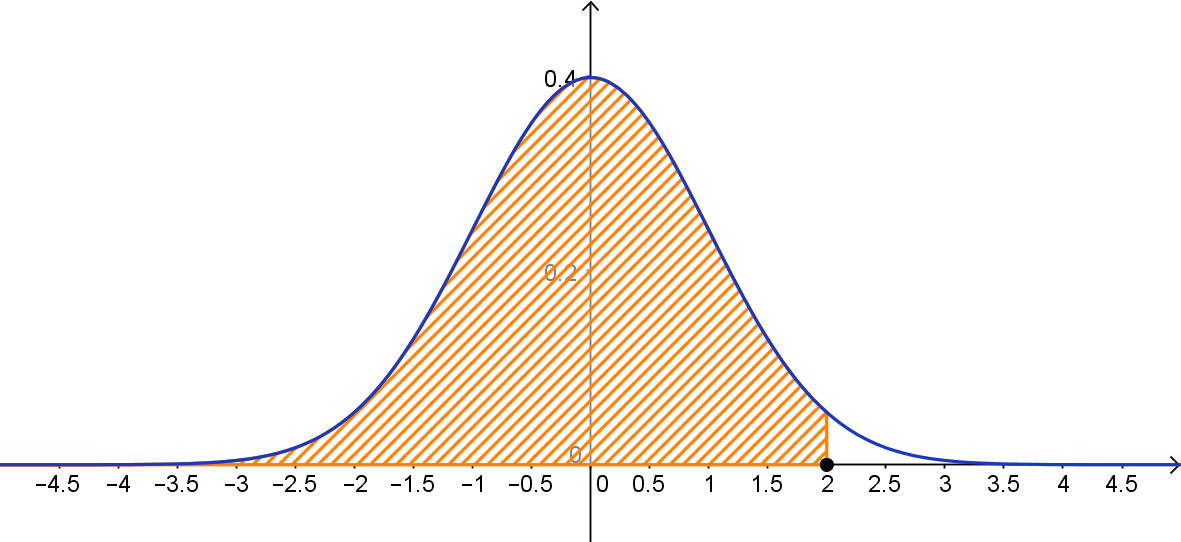
\includegraphics[width=9cm]{../fig/Cap06-ColaIzquierdaZ-02.png}\\
(b1)\\
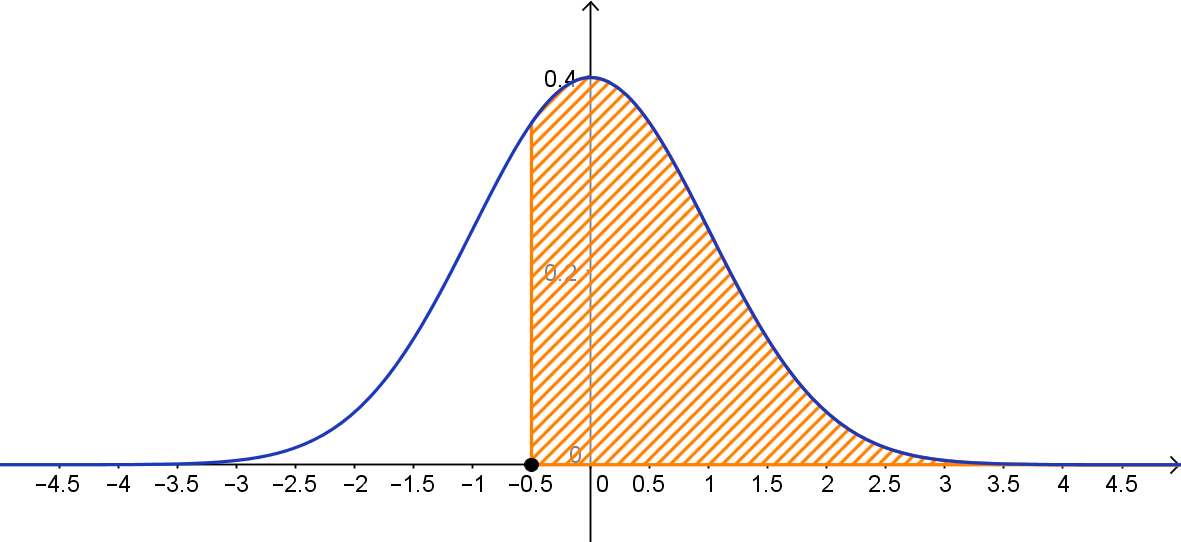
\includegraphics[width=9cm]{../fig/Cap06-ColaDerechaZ-01.png}\\
(b2)\\
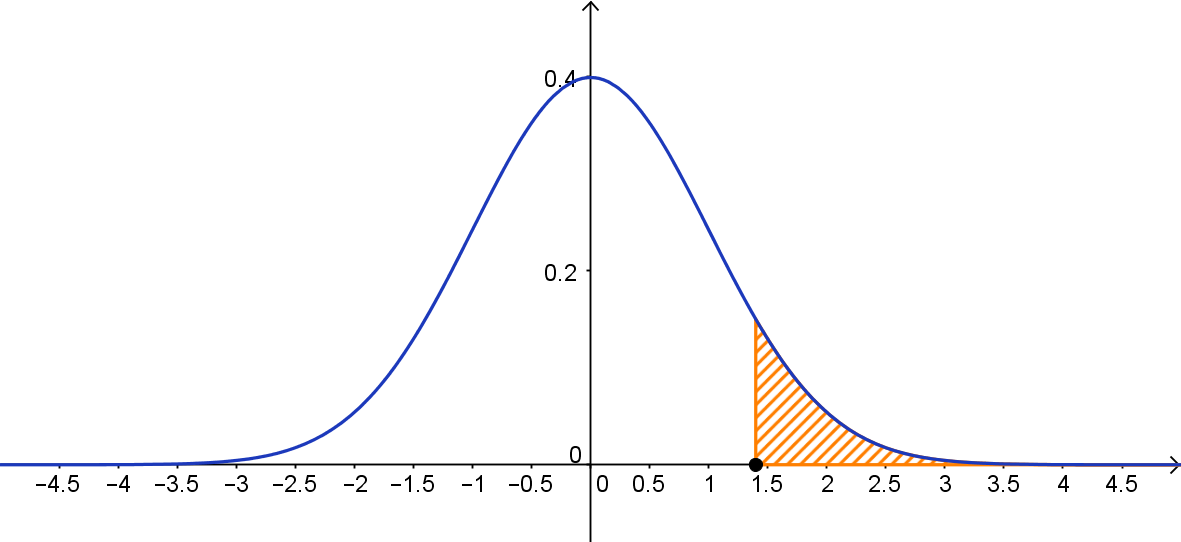
\includegraphics[width=9cm]{../fig/Cap06-ColaDerechaZ-02.png}\\
\end{tabular}
\end{enColor}
\begin{bn}
\begin{tabular}{c}
(a1)\\
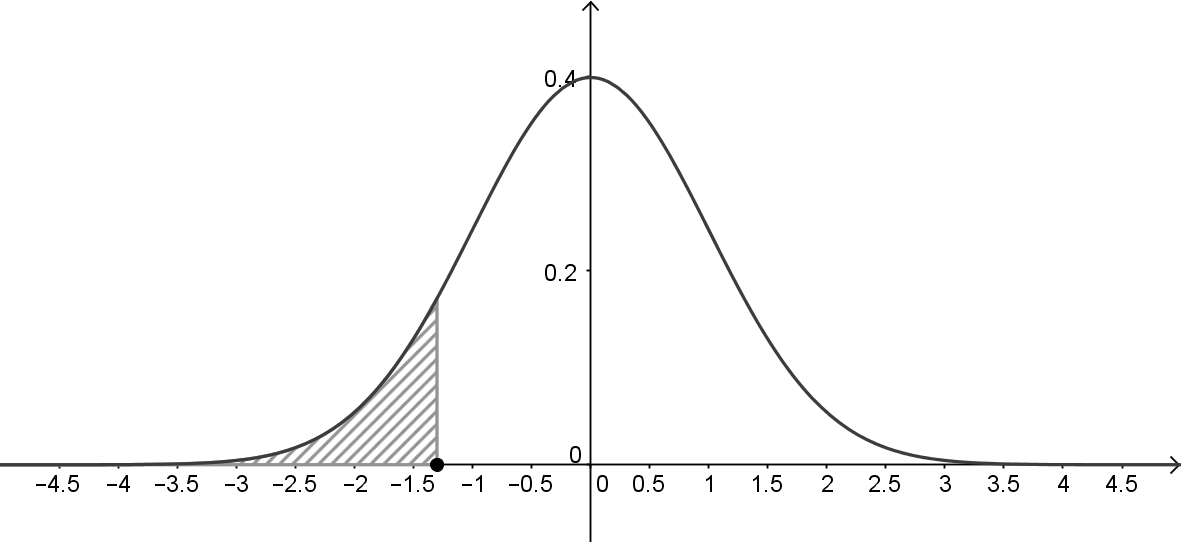
\includegraphics[width=9cm]{../fig/Cap06-ColaIzquierdaZ-01-bn.png}\\
(a2)\\
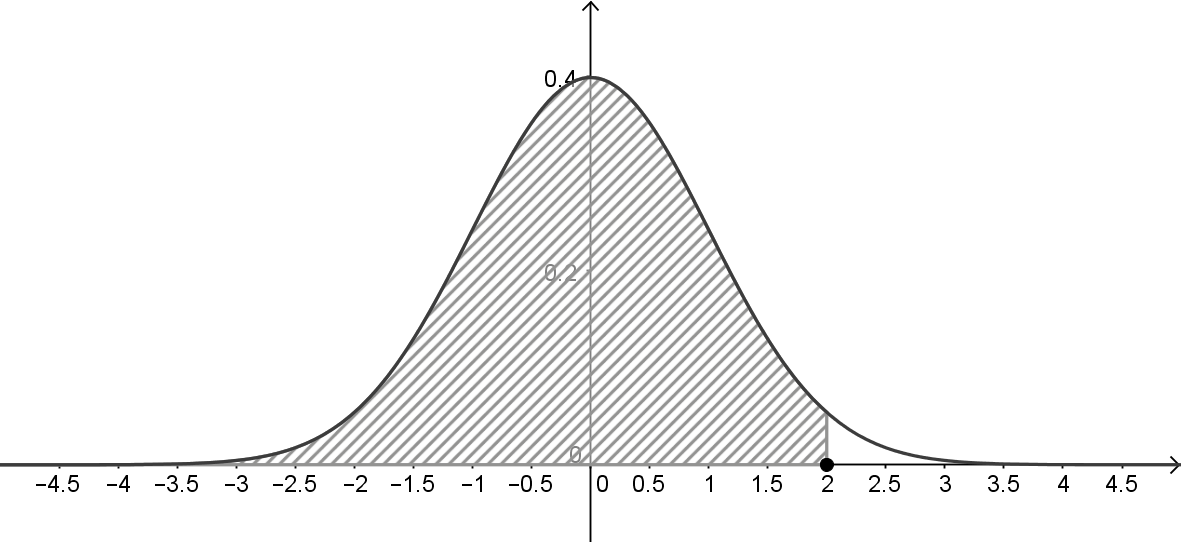
\includegraphics[width=9cm]{../fig/Cap06-ColaIzquierdaZ-02-bn.png}\\
(b1)\\
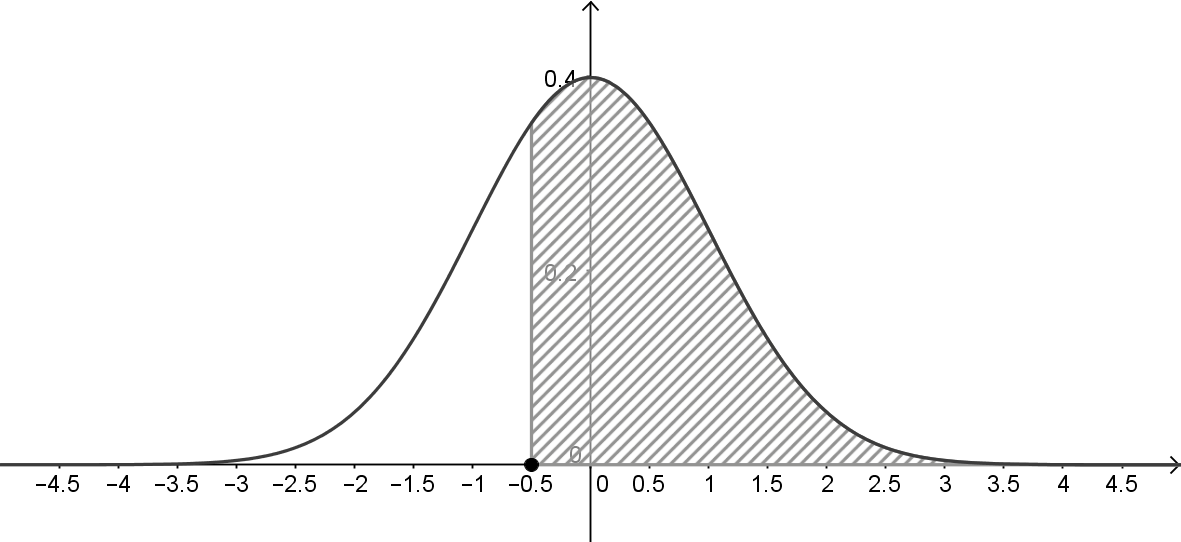
\includegraphics[width=9cm]{../fig/Cap06-ColaDerechaZ-01-bn.png}\\
(b2)\\
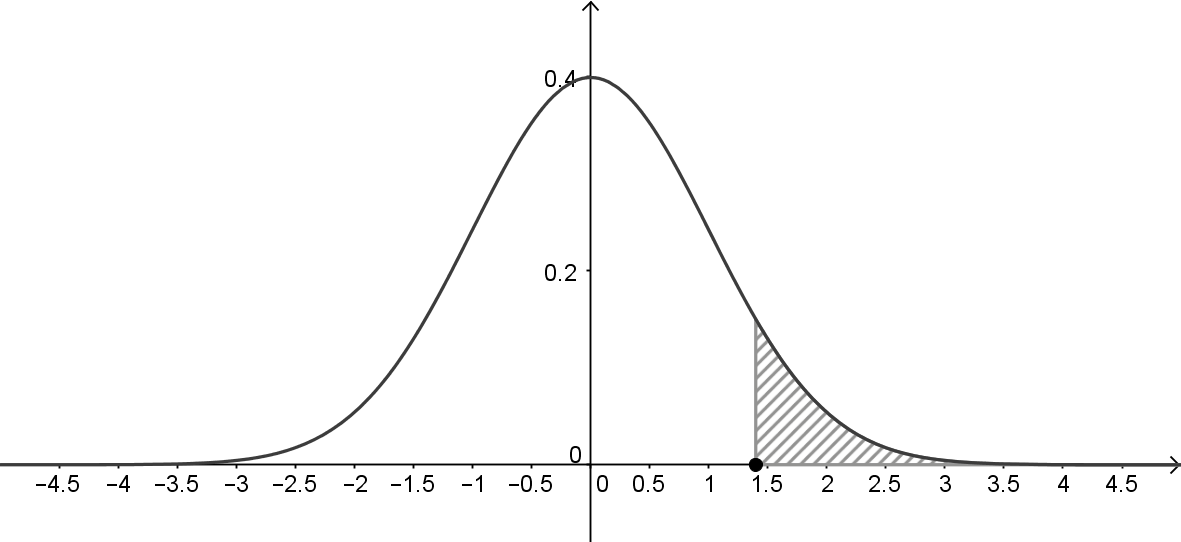
\includegraphics[width=9cm]{../fig/Cap06-ColaDerechaZ-02-bn.png}\\
\end{tabular}
\end{bn}
\caption{Problemas (directos) de probabilidad sobre colas de $Z$.
Los dos primeros son colas izquierdas: (a1) $P(Z<-1.3)$, (a2) $P(Z<2)$. Los dos últimos, colas derechas: (b1) $P(Z>-0.5)$, (b2) $P(Z>1.4)$. En todos los casos, queremos calcular el área sombreada.
}
\label{cap06:fig:ProblemasColasZ}
\end{center}
\end{figure}

Los {\sf problemas inversos}\index{problemas inversos, Z} de probabilidad se
caracterizan porque el valor de partida, el dato que tenemos, es una {\em
probabilidad}. Y lo que buscamos, ahora, son los {\em valores que producen esa
probabilidad}.

\begin{ejemplo}
\label{cap06:ejem:ProblemaInversoProbabilidadZ}
Un ejemplo típico sería esta pregunta:
\begin{center}
¿Cuál es el valor $a$ para el que se cumple $P(Z>a)=0.25$?
\end{center}
Este ejemplo se ilustra en la Figura \ref{cap06:fig:ProblemaInversoZ}. En el Tutorial06 veremos que, aproximadamente, $a = 0.6745$.\qed
\begin{figure}[h!]
\begin{center}
\begin{enColor}
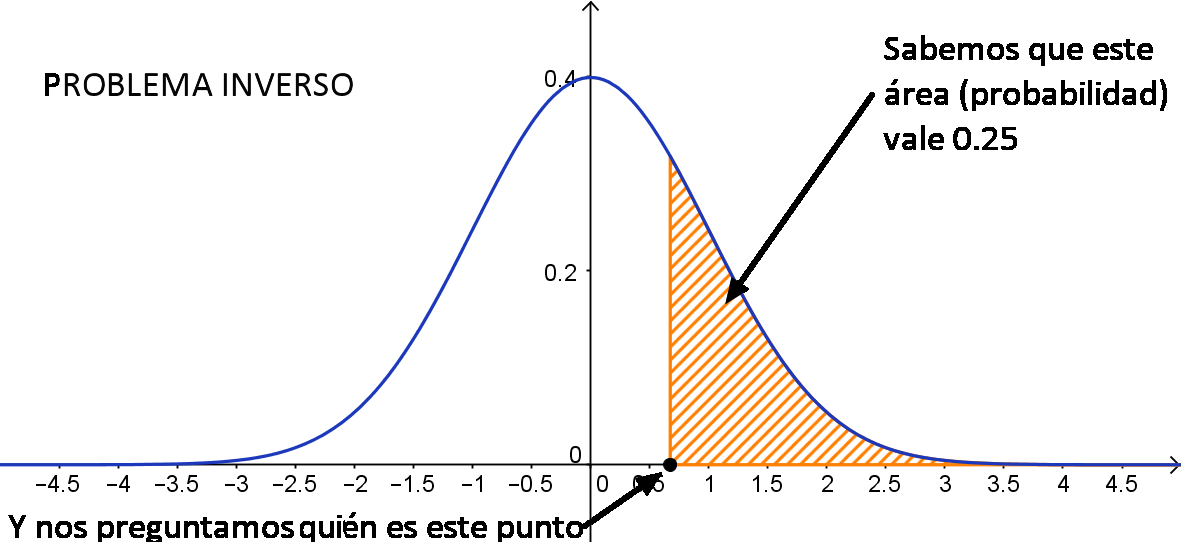
\includegraphics[width=13cm]{../fig/Cap06-ProblemaInversoZ-01.png}
\end{enColor}
\begin{bn}
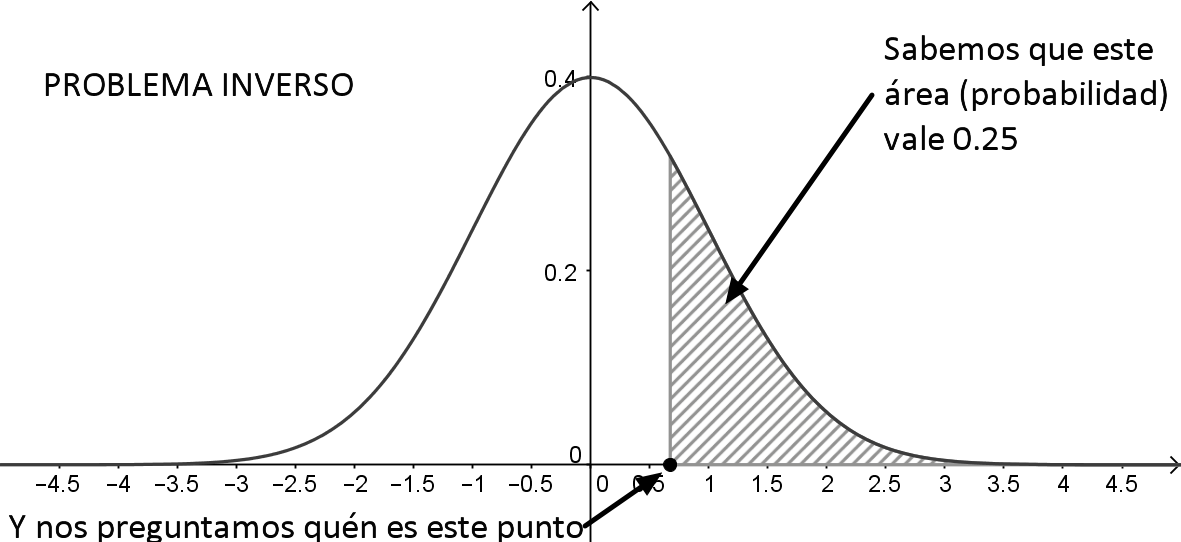
\includegraphics[width=13cm]{../fig/Cap06-ProblemaInversoZ-01-bn.png}
\end{bn}
\caption{Un problema inverso de probabilidad en $Z$.}
\label{cap06:fig:ProblemaInversoZ}
\end{center}
\end{figure}
\end{ejemplo}

Los problemas inversos se dividen, a su vez, en dos tipos, de forma muy
parecida a lo que sucedía con los directos. Ahora, por razones que se verán
enseguida, empezamos por las colas. En todos los casos, se supone que $p_0$ es
un valor conocido de probabilidad (un dato del problema):
\begin{itemize}
  \item Preguntas sobre la probabilidad de una {\sf cola} de la distribución
      normal. Es decir, preguntas de una de estas dos formas:
      \[
      \begin{cases}
      \mbox{¿Para qué valor $a$ se cumple $P(Z>a)=p_0$?}& \quad\mbox{(cola derecha)}.\\[3mm]
      \mbox{¿Para qué valor $a$ se cumple $P(Z<a)=p_0$?}& \quad\mbox{(cola izquierda)}.
      \end{cases}
      \]

  \item En este caso, las preguntas sobre intervalos las vamos a hacer
      siempre sobre intervalos simétricos (de lo contrario no habría una
      respuesta única). Serán preguntas de la forma:
      \begin{center}
      ¿Para qué valor $K$ se cumple $P(-K<Z<K)=p_0$?
      \end{center}
\end{itemize}

La misma Figura \ref{cap06:fig:ProblemasColasZ} (pág.
\pageref{cap06:fig:ProblemasColasZ}), que ya usamos para los problemas
directos, puede servir de ilustración de los problemas sobre colas. Lo
importante es entender que, en este caso, sabemos cuanto vale el area
sombreada, y lo que necesitamos averiguar es dónde hay que situar el punto del
eje horizontal para obtener ese valor del área.

Probablemente, el lector habrá reconocido el problema inverso sobre los
intervalos simétricos. Es exactamente el problema que dejamos pendiente al
final del apartado anterior, y que dijimos que era la pieza clave que faltaba
para el cálculo de los intervalos de confianza. Por esa razón, le vamos a
prestar una atención especial en lo que resta de apartado.
%Antes de empezar con
%esto, un comentario. Puesto que vamos a usar R como herramienta básica de
%trabajo con el ordenador, creemos conveniente adelantar algunas cosas. En R
%existen funciones para resolver problemas directos e inversos, {\em usando
%siempre la cola izquierda}. Además, las funciones que resuelven problemas
%directos empiezan siempre por {\tt p} (de probabilidad), mientras que las que
%resuelven problemas inversos empiezan siempre por {\tt q} (de quantile). El
%resto del nombre de la función se refiere a la distribución con la que estamos
%trabajando. Por ejemplo, la función que resuelve problemas directos de
%probabilidad en la distribución normal es {\tt pnorm}, mientras que para los
%problemas inversos de la normal tenemos {\tt qnorm}. Si trabajamos con una
%distribución binomial usaremos {\tt pbinom} y {\tt qbinom} para problemas
%directos e inversos, respectivamente.


Recordemos que, como aparecía en la Ecuación
\ref{cap06:ecu:ValorKIntervalo90EnZ} (pág
\pageref{cap06:ecu:ValorKIntervalo90EnZ}), se trata de calcular un valor $K$
tal que:
\[P(-K< Z <K)=0.9\]
Este problema se ilustra en la Figura
\ref{cap06:fig:ProblemaInversoZIntervalo90}.

\begin{figure}[h!]
\begin{center}
\begin{enColor}
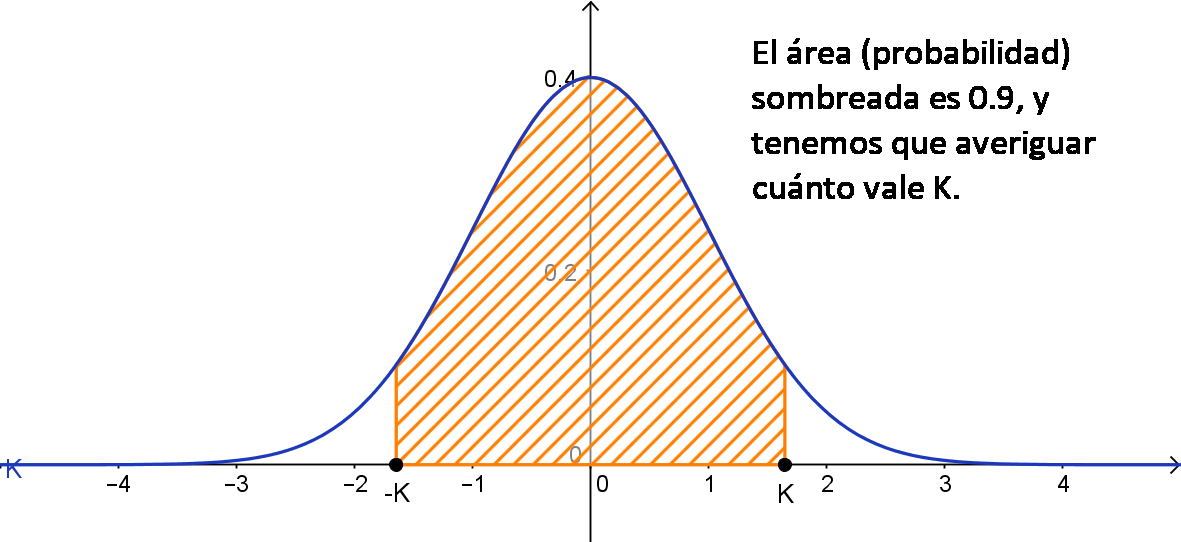
\includegraphics[width=13cm]{../fig/Cap06-ProblemaInversoZ-02.png}
\end{enColor}
\begin{bn}
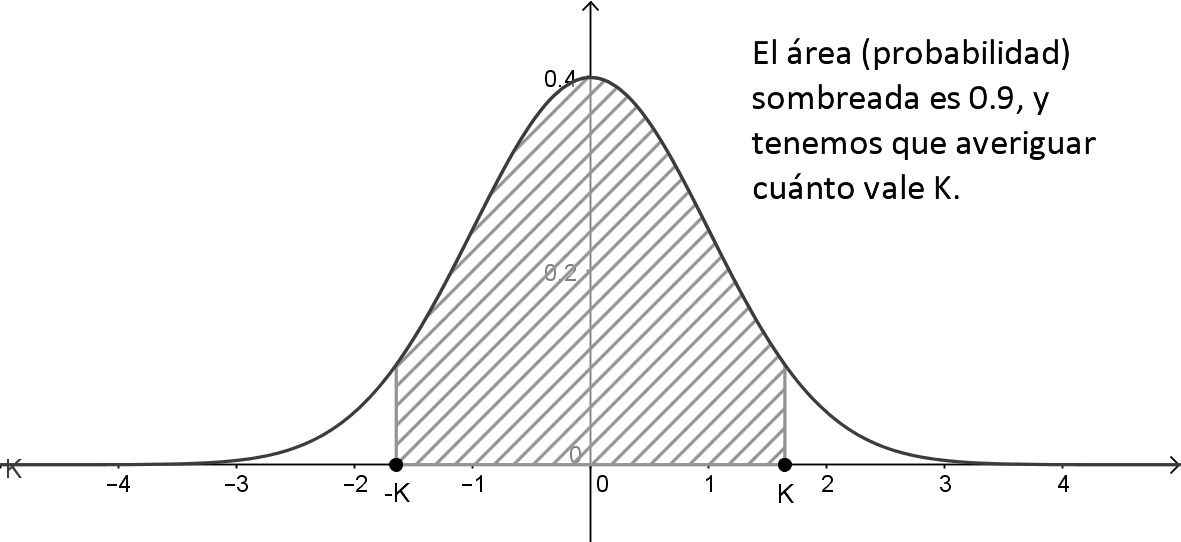
\includegraphics[width=13cm]{../fig/Cap06-ProblemaInversoZ-02-bn.png}
\end{bn}
\caption{El paso clave en la construcción de un intervalo de confianza al 90\%.}
\label{cap06:fig:ProblemaInversoZIntervalo90}
\end{center}
\end{figure}
%
%\begin{center}
%\begin{figure}
%	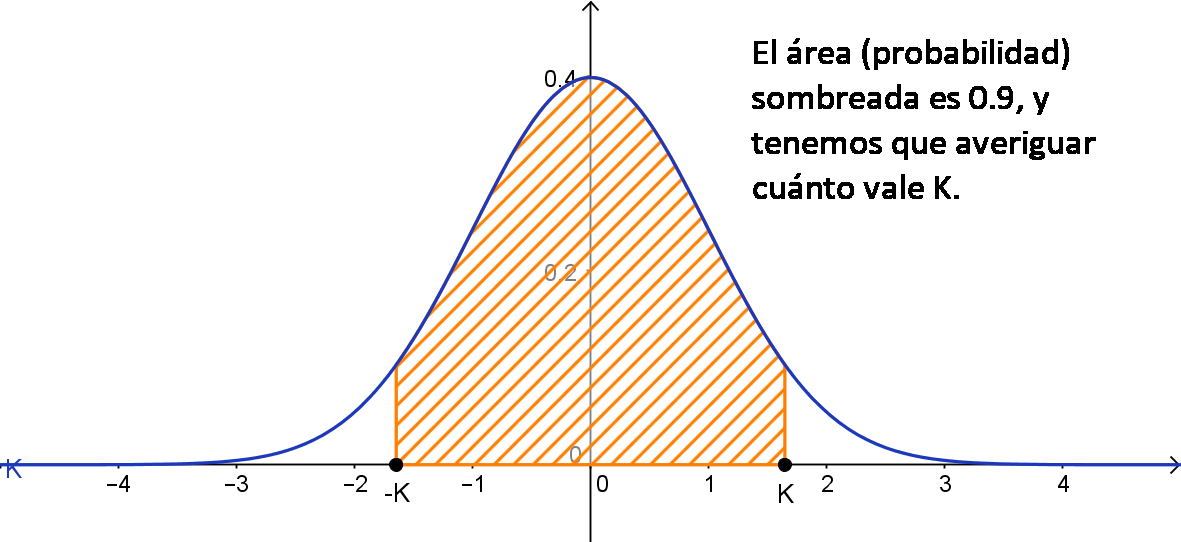
\includegraphics[width=13cm]{../fig/Cap06-ProblemaInversoZ-02.png}
%	\caption{}
%    \label{}				
%\end{figure}
%\end{center}

Vamos a introducir la terminología y notación que usaremos para esta situación,
y que, con pequeñas variaciones, usaremos en otros capítulos del curso. El
valor $0.9$, al que a menudo nos referiremos, indistintamente, como ``el
90\%'', medirá la probabilidad de que el intervalo de confianza contenga de
hecho a la media $\mu$. Ese valor, $nc=0.9$, es lo que llamaremos el {\sf nivel
de confianza}\index{nivel de confianza, $nc=1-\alpha$}\index{$nc$} del
intervalo, y usaremos el símbolo $nc$ para representarlo. Los niveles de
confianza habituales en las aplicaciones son $0.9$, $0.95$ y $0.99$, aunque en
principio puede usarse cualquier valor de probabilidad como nivel de confianza.
Junto con el nivel de confianza, en Estadística se utiliza el
valor\index{$\alpha=1-nc$}
\[\alpha=1-nc,\]
que es el {\em complemento a uno} de $nc$. De esa forma, si el nivel de
confianza es $nc=0.90$, entonces $\alpha=0.10$. En el contexto de la Figura
\ref{cap06:fig:ProblemaInversoZIntervalo90}, $nc=0.9$ representa el área
sombreada, mientras que $\alpha=0.1$ es el área restante, que en este caso es
la suma de las dos colas izquierda y derecha, definidas respectivamente por
$-K$ y $K$. Ahora vamos a usar uno de esos trucos típicos de las distribuciones
continuas. Puesto que la gráfica de $Z$ es simétrica respecto del eje vertical,
las dos colas son iguales. Y si tienen que sumar $\alpha=0.10$, a cada una de
ellas le corresponde $\dfrac{\alpha}{2}=0.05$. Volviendo a la Figura
\ref{cap06:fig:ProblemaInversoZIntervalo90}, el valor $K$ que buscamos deja en
la cola derecha una probabilidad igual a $\dfrac{\alpha}{2}=0.05$, y deja en su
cola izquierda una probabilidad igual a $1-\dfrac{\alpha}{2}=0.95$.

Este razonamiento nos permite convertir el problema inverso de intervalos de la
Figura \ref{cap06:fig:ProblemaInversoZIntervalo90} en un problema inverso, pero
ahora sobre colas, como el de la Figura \ref{cap06:fig:ProblemaInversoZ}. Y eso
es muy útil, porque las tablas de valores de $Z$ que se usaban antes,
así como muchos programas de ordenador, están pensados para resolver problemas
inversos de colas, no de intervalos. No sólo en la normal, sino en todas las distribuciones que
vamos a ver. Esto, que al principio puede parecer una limitación, se agradece
al poco tiempo, porque aporta coherencia y método a nuestro trabajo.
Empezaremos a practicar esto de forma detallada en los Tutoriales porque, a lo
largo del curso, vamos a pasar muchas veces (de verdad, muchas) por este camino,
que lleva desde el nivel de confianza $nc$, pasando por $\alpha$, hasta llegar
al problema inverso de probabilidad que, de hecho, tenemos que resolver usando
el ordenador, y que, en el caso que nos ocupa es:
\begin{center}
{\em ¿Cuál es el valor de $Z$ que deja en su cola izquierda una probabilidad
igual a $1-\dfrac{\alpha}{2}$?}
\end{center}
Hasta ahora hemos llamado $K$ a ese valor, pero hay una notación mejor.

    \begin{center}
    \fcolorbox{black}{Gris025}{
    \begin{minipage}{12.5cm}
        \begin{center}
        %%%%%%%%%%%%%%%%%%%%%%%%%%%%%%%%%%%%%%%
        {\bf  Valores críticos $z_p$ de la normal estándar $Z$.}\\
        \end{center}
        \index{valores críticos de $Z$}
        \index{$z_p$, $z_{\alpha}$ valor crítico de $Z$}
       %%%%%%%%%%%%%%%%%%%%%%%%%%%%%%%%%%%%%%%
       Sea $0\leq p\leq 1$ un valor de probabilidad cualquiera. El {\sf valor crítico} de $Z$ correspondiente a $p$ es el valor $z_p$ que
       cumple:
       \begin{equation}\label{cap06:ecu:DefinicionValorCriticoZ}
       F(z_p)=P(Z\leq z_p)=1-p.
       \end{equation}
       Aquí $F$ es la función de distribución de $Z$ (en el sentido de la Sección \ref{cap05:sec:FuncionDistribucionVariableContinua}). Gráficamente, $z_p$ es el valor que deja una probabilidad $p$ en su cola derecha (es decir, $1-p$ en la cola izda.) Ver la Figura
       \ref{cap06:fig:ValorCriticoZ} (a).

       En particular, para el intervalo de confianza para la media usamos el valor crítico $z_{\alpha/2}$, que
       satisface (ver la Figura \ref{cap06:fig:ValorCriticoZ} (b)):
       \[F\left(z_{\alpha/2}\right)=P\left(Z\leq z_{\alpha/2}\right)=1-\dfrac{\alpha}{2},\]
       y que, por lo tanto, deja en su cola derecha una probabilidad igual a $\dfrac{\alpha}{2}$.
       %%%%%%%%%%%%%%%%%%%%%%%%%%%%%%%%%%%%%%%
    \end{minipage}}
    \end{center}

%La Figura \ref{cap06:fig:ValorCriticoZ} ilustra esta definición.

\begin{figure}[h!]
\begin{center}
\begin{enColor}
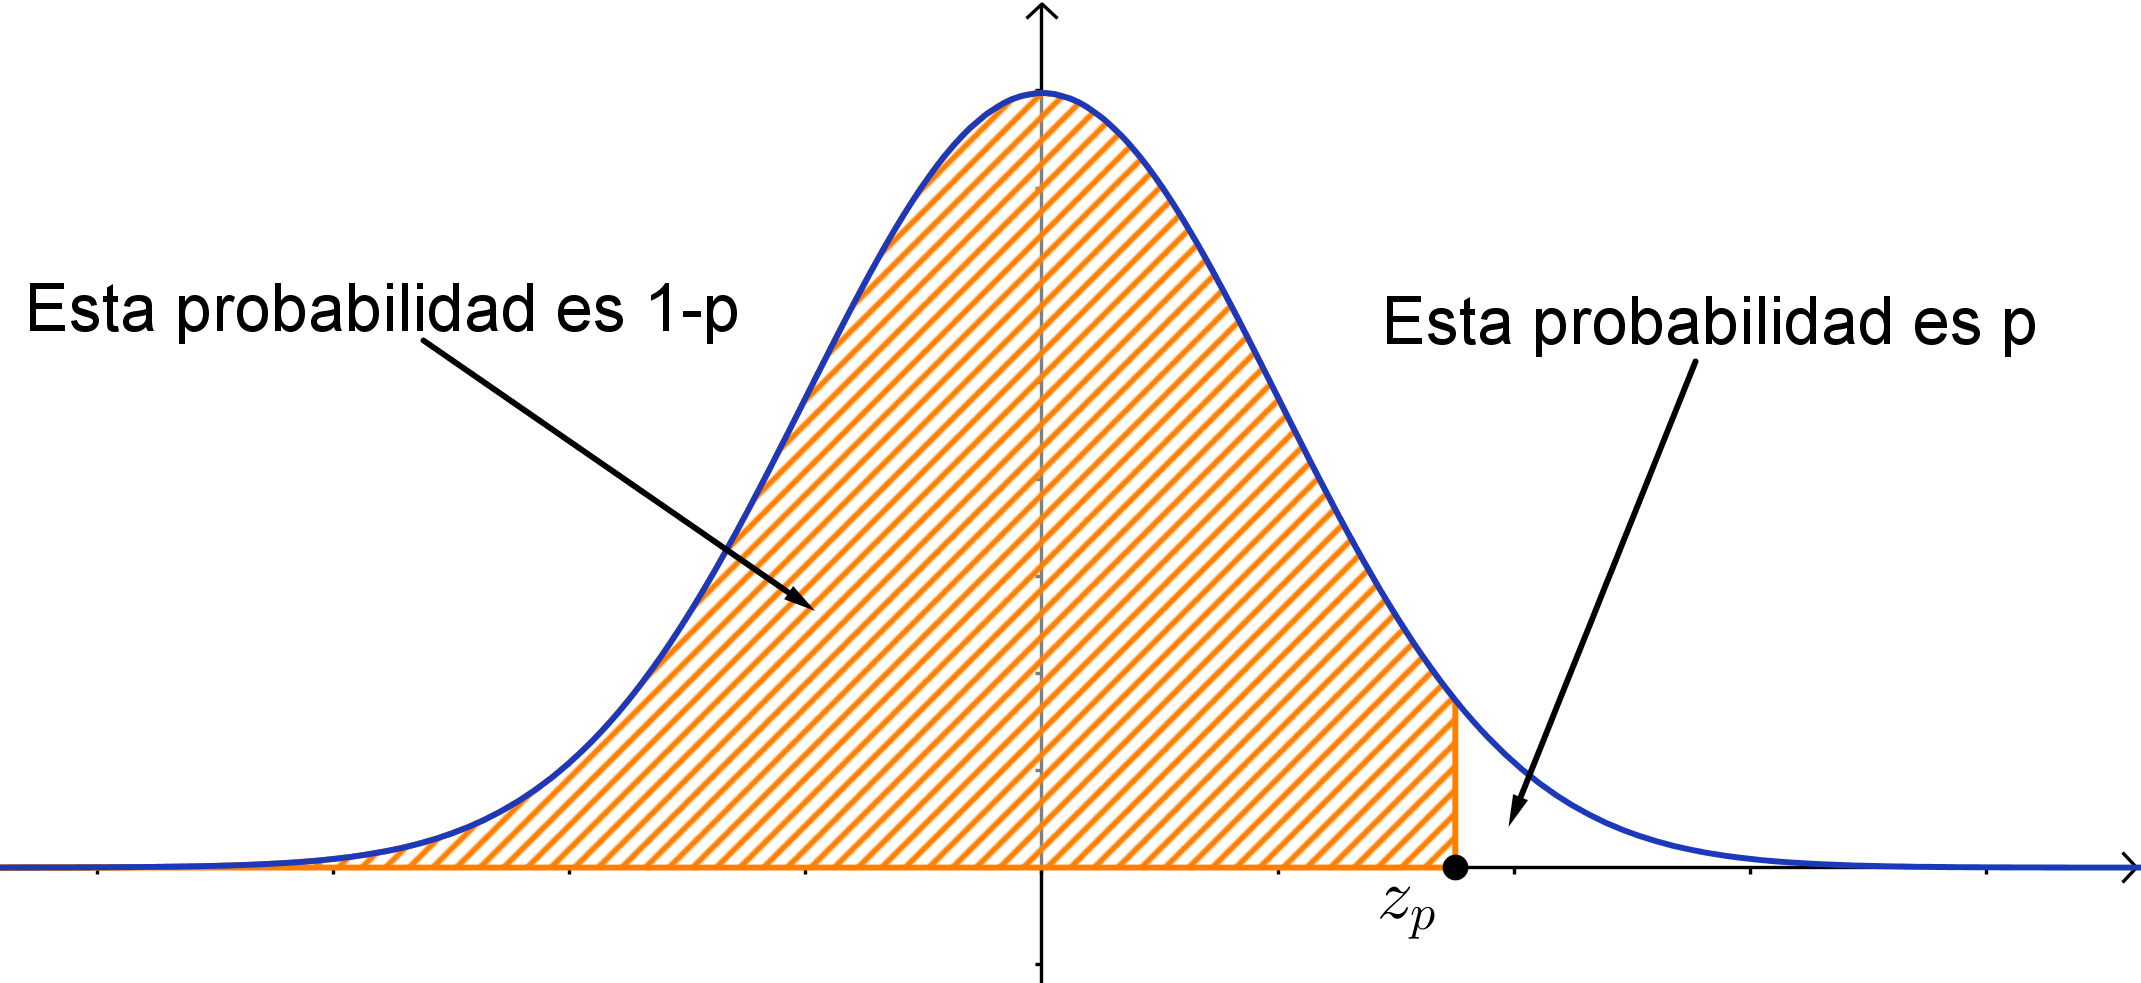
\includegraphics[width=13cm]{../fig/Cap06-ValoresCriticosZ.png}\\
(a)\\[5mm]
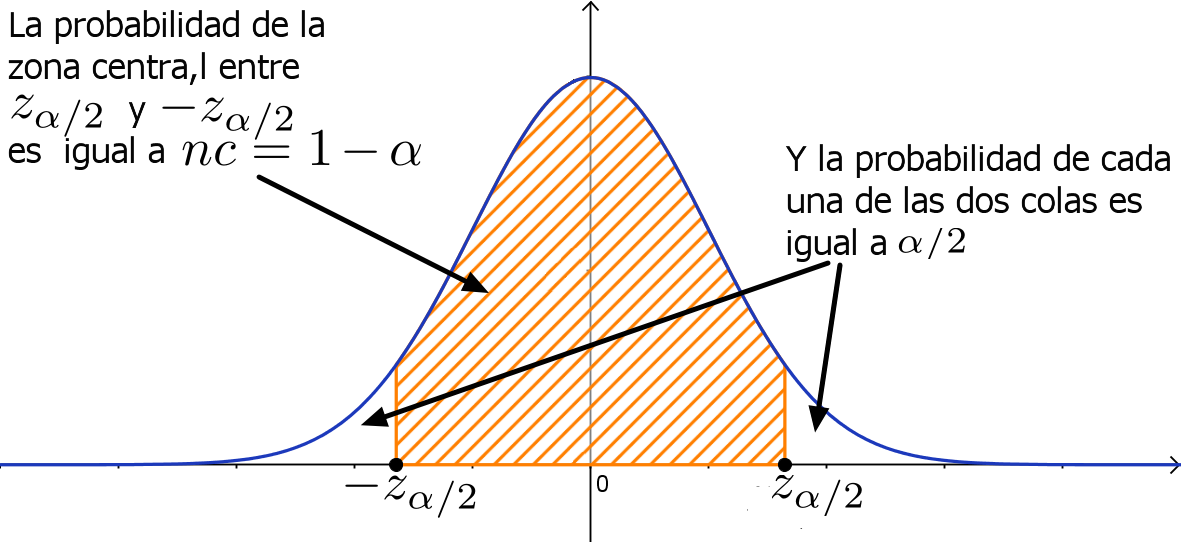
\includegraphics[width=13cm]{../fig/Cap06-InterpretacionValorCriticoZ.png}\\
(b)
\end{enColor}
\begin{bn}
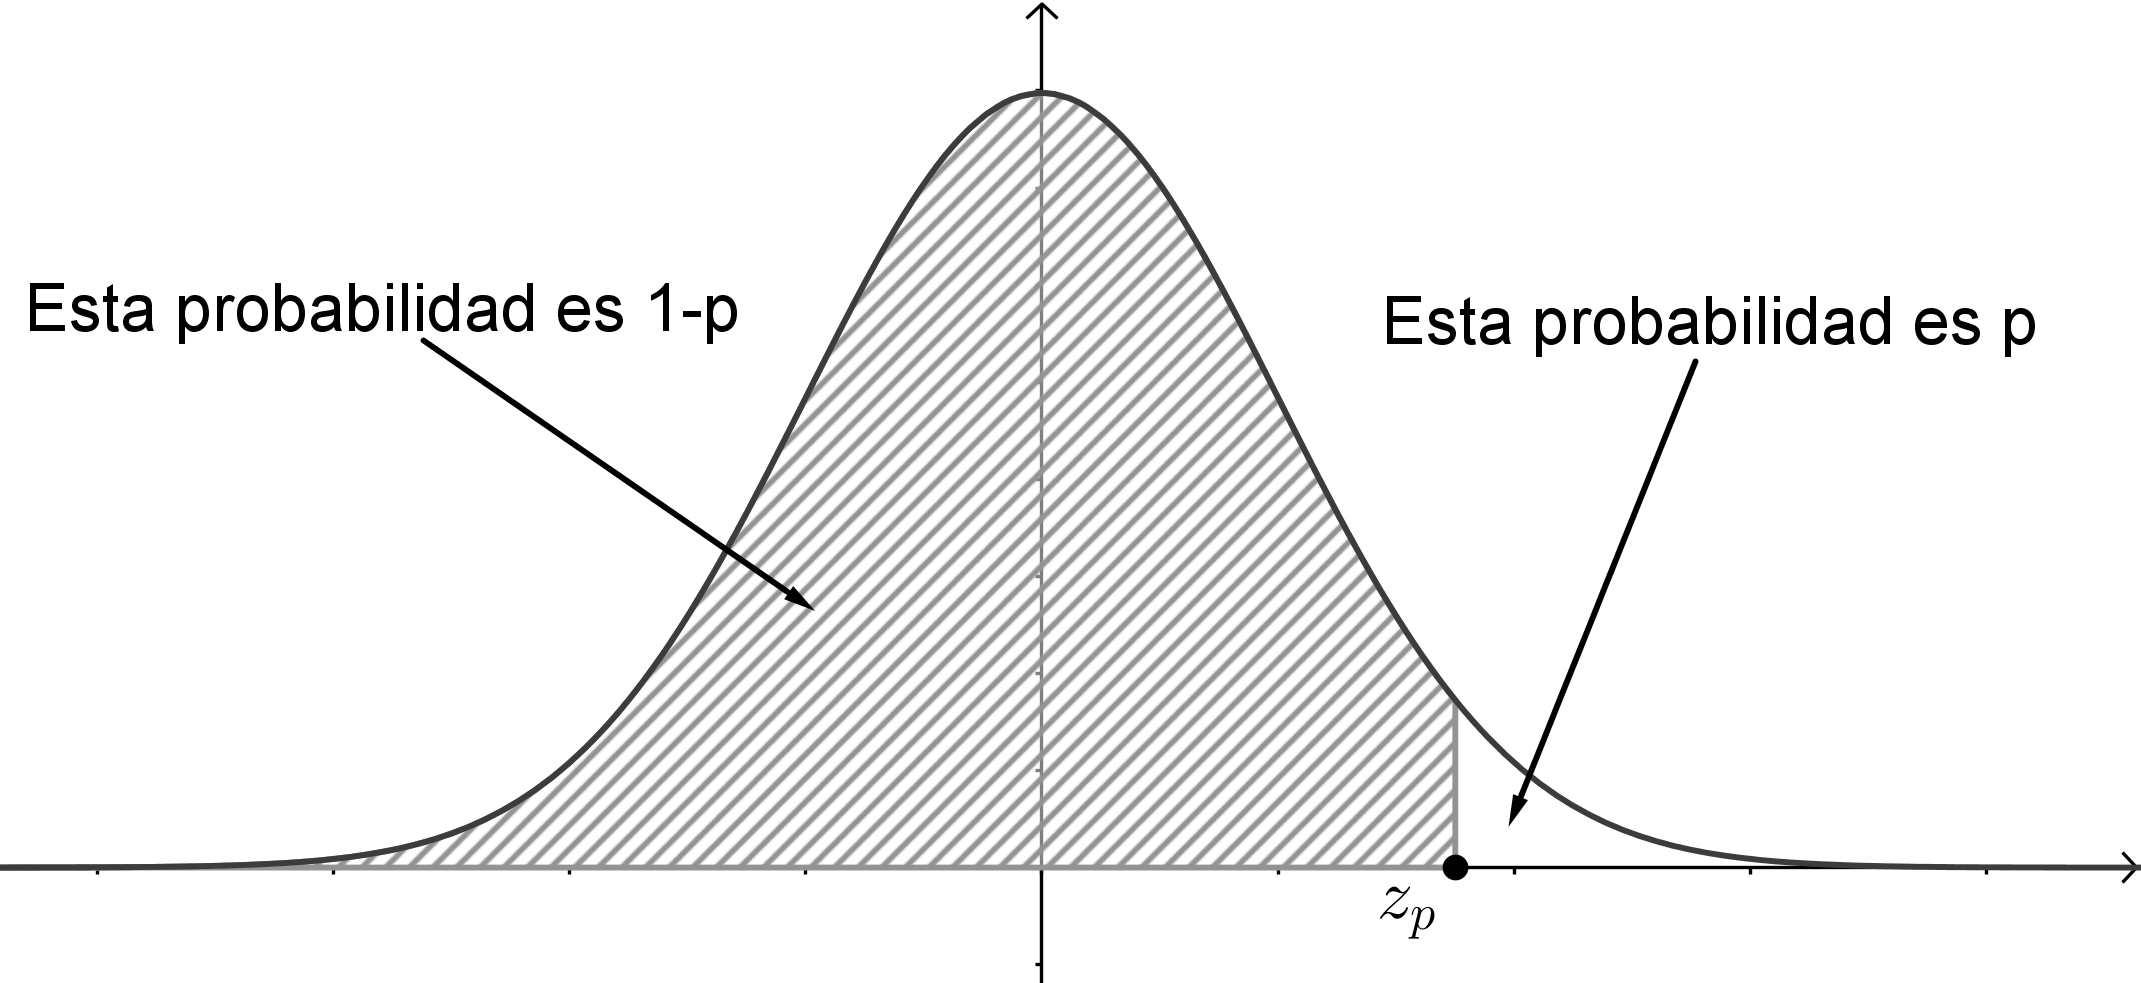
\includegraphics[width=13cm]{../fig/Cap06-ValoresCriticosZ-bn.png}\\
(a)\\[5mm]
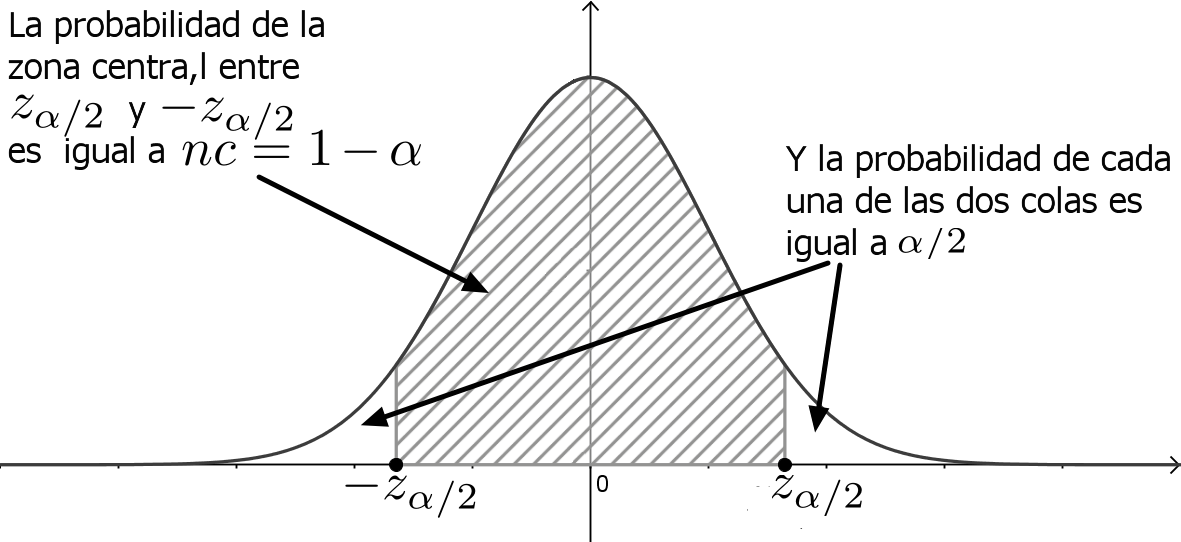
\includegraphics[width=13cm]{../fig/Cap06-InterpretacionValorCriticoZ-bn.png}\\
(b)
\end{bn}
\caption{Representación gráfica de los valores críticos de la normal estándar $Z$:
(a) significado de $z_p$ para cualquier $p$, (b) significado del valor $z_{\alpha/2}$ que se
usa en los intervalos de confianza para $\mu$.}
\label{cap06:fig:ValorCriticoZ}
\end{center}
\end{figure}
%

Al principio todo este asunto del $\alpha$, el $1-\alpha$ y el $\alpha/2$,
resulta sin duda un poco confuso, y los errores son frecuentes. Hay dos
remedios que podemos recomendar para aliviar un poco este lance. El primero,
como siempre, es la práctica y el ejercicio. Pero en este caso, recomendamos
encarecidamente acompañar siempre nuestros razonamientos de un dibujo, una
representación gráfica por esquemática que sea, que nos ayude a traducir lo que
queremos obtener, en una pregunta que realmente sepamos responder
(generalmente, usando el ordenador). Además, recomendamos al lector
familiarizarse con los valores críticos $z_{\alpha/2}$ necesarios para los
intervalos de confianza más utilizados, y que aparecen en la Tabla
\ref{cap06:tabla:valoresCriticosZ}.
\begin{table}[h!]
\begin{center}
\begin{tabular}{|c|c|c|c|c|}
\hline
{\bf Nivel de confianza:}\rule{0cm}{0.5cm}&0.80&0.90&0.95&0.99\\
\hline
$z_{\alpha/2}$\rule{0cm}{0.5cm}&$1.28$&$1.64$&$1.96$&2.58\\[3mm]
\hline
\end{tabular}
\end{center}
\label{cap06:tabla:valoresCriticosZ}
\caption{Valores críticos de $Z$ más usados en intervalos de confianza. Esta tabla sólo tiene un valor orientativo: se muestran únicamente tres cifras significativas, y {\bf se desaconseja} usar tan pocas cifras en los cálculos.}
\end{table}

\subsubsection{Notación para la función de distribución de una variable normal}
\label{ch06:subsubsec:NotacionPhiFuncionDistribucionZ}

Hemos reservado el símbolo $Z$ para la normal estándar, porque esa distribución ocupa un lugar destacado en la Estadística. Por  la misma razón, no es de extrañar que se use una notación especial para su función de distribución (en lugar del símbolo genérico $F$ que venimos usando). Concretamente, escribiremos:
\begin{equation}
\label{ch06:ecu:NotacionPhiFuncionDistribucionZ}
\Phi(x) = P(Z < z).
\end{equation}
De esa manera, el símbolo $\Phi$\index{$\Psi$}\index{función de distribución de la normal estándar $Z$} siempre representará la función de distribución de la variable  $Z$. Para los puntos críticos se tiene, entonces:
\[\Phi\left(z_{p}\right)=1-p.\]
De forma análoga, si $X\sim N(\mu,\sigma)$ es una variable normal cualquiera, usaremos el símbolo $\Phi_{\mu,\sigma}$\index{$\Phi_{\mu,\sigma}$}  para referirnos a su función de distribución. Por lo tanto, se tiene:
\[\Phi_{\mu,\sigma}(x) = P(X < x), \qquad \mbox { para } X\sim N(\mu,\sigma).\]


\subsection{Construcción del intervalo de confianza.}
\label{cap06:subsec:ConstruccionIntervaloConfianza}

Ahora que ya disponemos del lenguaje de niveles de confianza y valores
críticos, podemos retomar la construcción del intervalo de confianza para la
media $\mu_X$, donde $X$ es una variable normal de tipo $N(\mu_X,\sigma_X)$.
Recordemos que, en el razonamiento que sigue a la Ecuación
\ref{cap06:ecu:ValorKIntervalo90EnZ} (pág.
\pageref{cap06:ecu:ValorKIntervalo90EnZ}), hemos visto que una vez encontrado
el valor $K$ que cumple:
    \[P(-K< Z <K)=0.9,\]
podemos usarlo para garantizar que se tiene:
    \[
    P\left(\bar X-K\cdot\dfrac{\sigma_X}{\sqrt{n}}< \mu_X<
    \bar X+K\cdot\dfrac{\sigma_X}{\sqrt{n}}\right)=0.9,
    \]
Y dejamos claro que sólo nos faltaba el valor de $K$, para obtener el intervalo
de confianza a partir de esto. En el apartado anterior hemos visto que ese
valor de $K$ tiene que cumplir
    \[P(Z\leq K)=0.95\]
Reformulando esto en nuestro nuevo lenguaje, empezamos con un nivel de
confianza $nc=0.9$. Entonces $\alpha=1-nc=0.1$. Por lo tanto,
$\dfrac{\alpha}{2}=0.05$, y el valor crítico correspondiente es $z_{0.05}$, que
satisface (ver la Ecuación \ref{cap06:ecu:DefinicionValorCriticoZ}):
    \[P(Z\leq z_{0.05})=1-0.05=0.95\]
En resumidas cuentas, $K=z_{0.05}$. Sustituyendo este valor, tenemos
    \[
    P\left(\bar X-z_{0.05}\cdot\dfrac{\sigma_X}{\sqrt{n}}< \mu_X<
    \bar X+z_{0.05}\cdot\dfrac{\sigma_X}{\sqrt{n}}\right)=0.9,
    \]
Y eso significa que el intervalo de confianza al 90\% para $\mu_x$ es este:
    \[
    \bar X-z_{0.05}\cdot\dfrac{\sigma_X}{\sqrt{n}}< \mu_X<
    \bar X+z_{0.05}\cdot\dfrac{\sigma_X}{\sqrt{n}}.
    \]
Si, en lugar del 90\%, utilizáramos cualquier otro nivel de confianza,
procederíamos de forma muy similar. Así que podemos extraer una conclusión
general, y añadir un poco más de terminología:
    \begin{center}
    \fcolorbox{black}{Gris025}{
    \begin{minipage}{12.5cm}
        \begin{center}
        %%%%%%%%%%%%%%%%%%%%%%%%%%%%%%%%%%%%%%%
        {\bf  Intervalo de confianza para la media $\mu$.}\\{\bf Población normal, con desviación típica conocida.}\\
        \end{center}
        \index{Intervalo de confianza para la media $\mu$, población $N(\mu,sigma)$, con $\sigma$ conocida.}
       %%%%%%%%%%%%%%%%%%%%%%%%%%%%%%%%%%%%%%%
        Sea $X$ una variable aleatoria normal, cuya desviación típica $\sigma_X$ se conoce. Si consideramos muestras de tamaño $n$, entonces el intervalo de confianza al nivel $nc=(1-\alpha)$  para la media $\mu_X$ es:
        \begin{equation}\label{cap06:ecu:IntervaloConfianzaMediaSigmaConocida}
        \bar X-z_{\alpha/2}\cdot\dfrac{\sigma_X}{\sqrt{n}}\leq \mu_X \leq \bar X+z_{\alpha/2}\cdot\dfrac{\sigma_X}{\sqrt{n}}.
        \end{equation}
        que, a menudo, escribiremos así:
        \[\mu_X =\bar X \pm z_{\alpha/2}\cdot\dfrac{\sigma_X}{\sqrt{n}}.\]
        El valor
        \begin{equation}\label{cap06:ecu:SemianchuraIntConfMediaConZ}
            z_{\alpha/2}\cdot\dfrac{\sigma_X}{\sqrt{n}},
        \end{equation}
        es la {\sf semianchura} del intervalo\index{semianchura, intervalo de confianza para $\mu$}, y si lo dividimos por el valor crítico, obtenemos el {\sf error estándar} de la muestra:
        \[\dfrac{\sigma_X}{\sqrt{n}}.\]
       %%%%%%%%%%%%%%%%%%%%%%%%%%%%%%%%%%%%%%%
    \end{minipage}}
    \end{center}
El procedimiento para obtener estos intervalos de confianza es, puramente
mecánico, y de hecho, en el Tutorial06 aprenderemos a automatizarlo lo más
posible, para evitar errores de cálculo. De momento, vamos a ver un ejemplo en
el que supondremos que ya sabemos cómo calcular los valores críticos
necesarios:
\begin{ejemplo}
\label{cap06:ejem:IntConfMediaSigmaConocida}
   Una muestra aleatoria de 50 individuos de una población normal, con varianza conocida, e igual a $16$, presenta una media muestral de $320$. Calcular un intervalo de confianza al $99\%$ para la media de la población.\\
   Usando cualquier herramienta de cálculo, o simplemente mirando la Tabla \ref{cap06:tabla:valoresCriticosZ}(pág. \pageref{cap06:tabla:valoresCriticosZ}), comprobamos que el valor crítico correspondiente a este nivel de confianza es:
   \[z_{\alpha/2}=2.58\]
   Calculamos la semianchura del intervalo:
   \[z_{\alpha/2}\cdot\dfrac{\sigma_X}{\sqrt{n}}=2.58\cdot\dfrac{4}{\sqrt{50}}\approx 1.46\]
   Y por lo tanto el intervalo de confianza buscado es:
   \[318.54\leq \mu_X\leq 321.46.\]
   o, escribiéndolo de otra forma:
   \[\mu=320\pm 1.46\]
   \quad\qed
\end{ejemplo}

%\pendiente{Me gustaría, antes de cerrar esta sección, ver una animación GeoGebra, que permita profundizar en la interpretación del concepto de intervalo de confianza, algo como el fichero
%\fichero{../datos/Cap06-InterpretacionIntervalosConfianza.ggb}{Cap06-InterpretacionIntervalosConfianza.ggb}. Pero no me acabo de fiar del generador de números aleatorios de GeoGebra, porque me salen muchos más intervalos defectuosos de los que esperaba. ¿Shiny?}

El cálculo de un intervalo de confianza para $\mu_X$ es, por lo tanto, un
asunto muy sencillo. Pero el resultado que hemos obtenido tiene dos debilidades
claras:\label{cap06:lugar:PreguntasIntervalosConfianza}
\begin{enumerate}
  \item Para aplicarlo, hemos supuesto que conocemos la desviación típica
      $\sigma_X$ de la variable. Y eso es, al menos, chocante. Estamos
      haciendo un intervalo de confianza para la (desconocida) media de $X$,
      ¿y se supone que conocemos su desviación típica?
  \item Además, estamos suponiendo que la población de partida es normal.
      ¿Qué sucede si no lo es? Sabemos que, para muestras suficientemente
      grandes, la segunda versión del Teorema Central del Límite (pág.
      \pageref{cap06:teo:TCLsegundaVersion}) nos garantiza que podremos
      seguir usando una normal para aproximar la media muestral $\bar X$.
      Pero ¿cuánto es {\em grande}?
\end{enumerate}
En el resto de este capítulo nos vamos a ocupar de estos dos problemas. Al
final tendremos una solución bastante completa para el problema de estimar
$\bar X$, al nivel introductorio de este curso, claro está.

\subsection{Interpretación probabilística del intervalo de confianza.}
\label{cap06:subsec:InterpretacionProbabilisticaIntervaloConfianza}

Aunque en los últimos apartados nos hemos dedicado, ante todo, a fijar el procedimiento para construir un intervalo de confianza para la media, no queremos seguir adelante sin insistir en la interpretación que hacemos de esos intervalos, sobre la que ya hemos hablado al comienzo de la Sección \ref{cap06:sec:IntervaloConfianzaMediaPoblacionNormal}. Cuando decimos que, a partir de una muestra de tamaño $n$, hemos construido un intervalo para la media con un nivel de confianza del $95\%$, lo que estamos diciendo es una afirmación probabilística {\em sobre el procedimiento que hemos utilizado}, referida al conjunto formado por todas las muestras de tamaño $n$. Y lo que estamos diciendo es que si selecciona una muestra al azar, y se usa este procedimiento, la probabilidad de que el intervalo que construimos contenga a la media es del $95\%$. Es decir, que de cada $100$ muestras elegidas al azar, es de esperar que $95$ de ellas, {\em cuando se usa este procedimiento}, darán como resultado un intervalo que contiene a la media real de la población.

\begin{figure}[p]
\begin{center}
\begin{enColor}
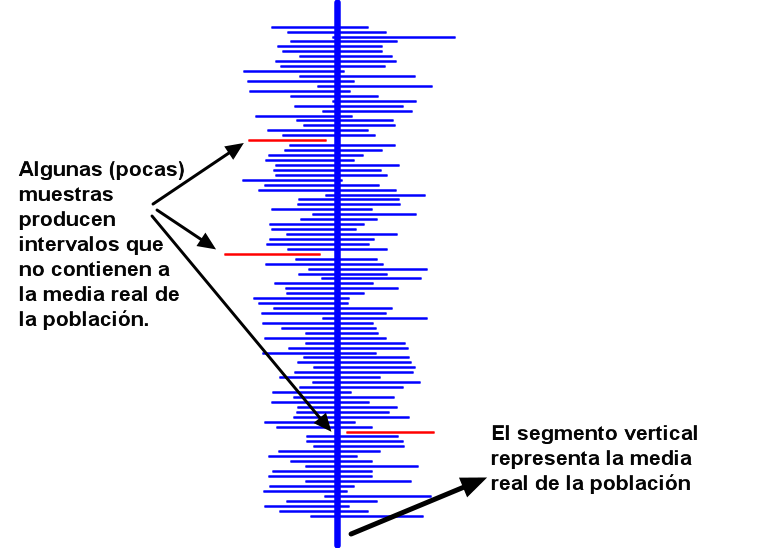
\includegraphics[width=14cm]{../fig/Cap06-InterpretacionIntervalosConfianza.png}
\end{enColor}
\begin{bn}
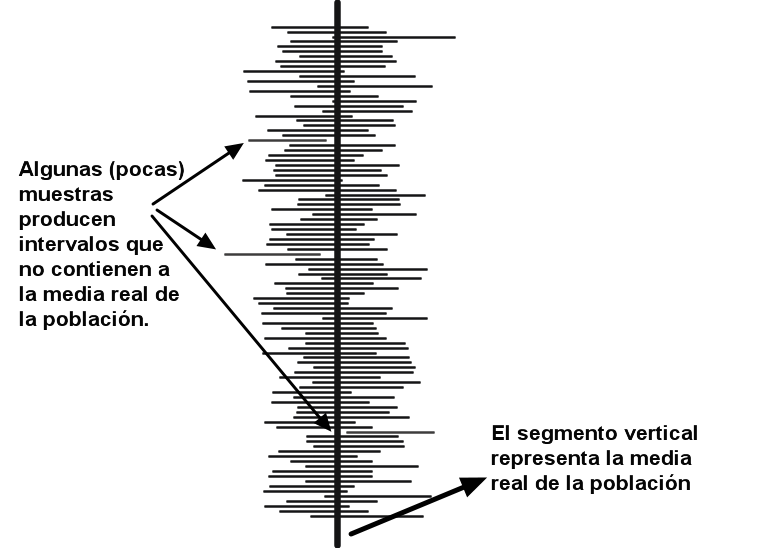
\includegraphics[width=14cm]{../fig/Cap06-InterpretacionIntervalosConfianza-bn.png}
\end{bn}
\caption{Interpretación probabilística de los intervalos de confianza.}
\label{cap06:fig:InterpretacionProbabilisticaIntervalosConfianza}
\end{center}
\end{figure}


Para ilustrar este punto, en la Figura \ref{cap06:fig:InterpretacionProbabilisticaIntervalosConfianza} (pág. \pageref{cap06:fig:InterpretacionProbabilisticaIntervalosConfianza}) hemos hecho precisamente esto: hemos elegido $100$ muestras al azar de una misma población normal (con $\mu=0$, $\sigma=0.1$), y hemos construido los $100$ intervalos de confianza correspondientes. El segmento vertical central indica la posición de la media real $\mu$ de la población. Y cada uno de los segmentos horizontales representa un intervalo de confianza, construido para una de esas muestras. Como puede verse, la inmensa mayoría de los segmentos horizontales, salvo algunos que hemos indicado con flechas, cortan al segmento vertical central. Es decir, la mayoría de los intervalos de confianza que hemos construido contienen a la media. Pero hay algunos pocos casos en los que no es así. Y no es porque esos intervalos estén {\em mal construidos}. Para construirlos se ha usado exactamente el mismo procedimiento que con cualquiera de los otros intervalos {\em ``correctos''}. El problema no está en el procedimiento, {\em sino en la muestra}. Como hemos discutido al hablar de la distribución muestral, un porcentaje (habitualmente pequeño) de muestras de tamaño $n$ se pueden considerar {\em muestras malas}, en el sentido de poco representativas de la población. Si al elegir una muestra al azar nos ha tocado en suerte una de esas ``muestras malas'', por más que apliquemos escrupulosamente el procedimiento que hemos descrito, es posible que terminemos con un intervalo de confianza que no contenga a la media de la población.

En particular, esto debería ayudar a aclarar un malentendido que se produce a veces, cuando decimos que  el intervalo $(a,b)$ es un intervalo de confianza  para $\mu$ al $95\%$.  A veces se leen argumentaciones como esta:
\begin{quote}
{\em Dado que el intervalo $(a,b)$ es un intervalo concreto, y el número $\mu$ es un número concreto, o bien $\mu$ pertenece al intervalo, o bien no pertenece.  Por ejemplo, dado el intervalo $(3,8)$ y el número $\mu=5$, está claro que $\mu$ pertenece a ese intervalo, y no tiene sentido decir que hay una probabilidad del $95\%$ de que $\mu=5$ pertenezca a $(3,8)$.}
\end{quote}
El problema con esta argumentación es que no se está entendiendo la interpretación probabilística del intervalo que acabamos de describir. Como todas las afirmaciones que se refieren a una probabilidad, la afirmación sobre el $95\%$ no puede interpretarse sin tener en cuenta el espacio probabilístico (el espacio $\Omega$, en el lenguaje del Capítulo \ref{cap:Probabilidad}) en el que estamos trabajando. En este caso concreto, como hemos dicho, esa afirmación se refiere al espacio de todas las muestras de tamaño $n$ de la población normal de referencia, y el valor del $95\%$, insistimos no se refiere (porque, en efecto, no tendría sentido hacerlo) a un intervalo concreto, sino al procedimiento de construcción de ese intervalo, y a nuestra estimación de la probabilidad de que ese procedimiento haya producido un intervalo que, de hecho, contenga a la media $\mu$.


\subsection{Cálculo del tamaño necesario de la muestra para alcanzar una precisión dada.}
\label{cap06:subsec:CalculoTamannoMuestra}

La información asociada al cálculo de un intervalo de confianza contiene siempre dos medidas de incertidumbre. Por un lado, como acabamos de discutir, la construcción del intervalo de confianza tiene un carácter probabilista (y en ese sentido, tiene que ver con la {\em exactitud} del método, en el sentido de la discusión de la Sección \ref{cap01:sec:PrecisionExactitudCifrasSignificativas}, pág. \pageref{cap01:sec:PrecisionExactitudCifrasSignificativas}). Pero, además, la anchura del intervalo del confianza es una medida adicional de la {\em precisión} con la que conocemos la posición de la media $\mu$. Naturalmente, lo ideal sería obtener un intervalo con un nivel de confianza muy alto, y una anchura muy pequeña. Pero, para un tamaño de muestra $n$ dado, ambas cantidades están relacionadas. Hemos visto, en la Ecuación \ref{cap06:ecu:SemianchuraIntConfMediaConZ} (pág. \pageref{cap06:ecu:SemianchuraIntConfMediaConZ}), que la semianchura del intervalo es
\[ z_{\alpha/2}\cdot\dfrac{\sigma_X}{\sqrt{n}},\]
y está claro que es esta cantidad la que define la precisión del intervalo. Pero también está claro que la semianchura depende de $\alpha$ (a través de $z_{\alpha/2}$), y por tanto, del nivel de confianza. Más concretamente: si se aumenta el nivel de confianza (que es $nc=1-\alpha$) acercando $nc$ a $1$, entonces $\alpha$ se acerca a $0$ y $z_{\alpha/2}$ aumenta. En resumen: {\em mientras $n$ esté fijo}, no podemos aumentar el nivel de confianza sin aumentar la anchura del intervalo, perdiendo precisión. Y viceversa, si queremos aumentar la precisión, y disminuir la anchura del intervalo, tenemos que rebajar su nivel de confianza.

Todo esta discusión, insistimos, parte de un tamaño fijo $n$ de la muestra. Pero precisamente el tamaño de la muestra es uno de los valores que el experimentador puede, en ocasiones, controlar. Y la Ecuación \ref{cap06:ecu:SemianchuraIntConfMediaConZ} de la semianchura muestra que, a medida que $n$ aumenta, como cabría esperar, la precisión del intervalo es cada vez mayor. Pero no sin esfuerzo: a causa de la raíz cuadrada, para disminuir a la mitad la anchura del intervalo, tenemos que multiplicar por cuatro el tamaño de la muestra.

En cualquier caso, la Ecuación \ref{cap06:ecu:SemianchuraIntConfMediaConZ} nos muestra una forma de conseguir un intervalo de confianza con la precisión y nivel de confianza deseados. El plan (provisional, como veremos) es este:
\begin{itemize}
  \item Fijamos un nivel de confianza, eligiendo $\alpha$, y calculamos $z_{\alpha/2}$.
  \item Fijamos la precisión deseada, que vamos a llamar $\delta$, y que no es otra cosa que la semianchura del intervalo:
      \begin{equation}\label{cap06:ecu:DeltaComoPrecisionIntConfMediaConZ}
        \delta=z_{\alpha/2}\cdot\dfrac{\sigma_X}{\sqrt{n}}
      \end{equation}
  \item Despejamos $n$, el tamaño de la muestra, de esta ecuación:
      \begin{equation}\label{cap06:ecu:TamannoMuestraIntConfMediaConZ}
        n=\left(z_{\alpha/2}\cdot\dfrac{\sigma_X}{\delta}\right)^2
      \end{equation}
\end{itemize}
Veamos un ejemplo:
\begin{ejemplo}
\label{cap06:ejem:DeterminacionTamannoMuestraIntConfConZ}
Una empresa farmacéutica está produciendo comprimidos, y como parte del control de calidad se desea medir el diámetro de esos comprimidos. Se sabe que el diámetro $X$ de los comprimidos sigue una distribución normal, con desviación típica $\sigma_X=1.3$mm. La empresa quiere una medida del diámetro con un error no mayor de $0.1$mm y un nivel de confianza del $99\%.$ ¿Qué tamaño de muestra debe utilizarse para conseguir ese objetivo?

Volviendo a la Ecuación \ref{cap06:ecu:TamannoMuestraIntConfMediaConZ}, lo que se ha hecho es fijar una precisión $\delta=0.1$mm. Además, al ser $nc=0.99$, tenemos $\alpha=0.01$, con lo que $\frac{\alpha}{2}=0.005$, y $z_{\alpha/2}=z_{0.1}\approx 2.58$ (usaremos más precisión para el cálculo real). Sustituyendo los valores:
\[
    n=\left(z_{\alpha/2}\cdot\dfrac{\sigma_X}{\delta}\right)^2
    \approx \left(2.58\cdot\dfrac{1.3}{0.1}\right)^2\approx 1121.3
\]
Naturalmente, no podemos tomar una muestra con un número fraccionario de comprimidos, así que la conclusión es que debemos tomar $n>1122$ para conseguir la precisión y nivel de confianza deseados.
\qed
\end{ejemplo}
Todo esto puede parecer muy satisfactorio, pero tiene un punto débil, que ya hemos señalado antes, y sobre el que nos vamos a extender en la siguiente Sección. El cálculo del intervalo de confianza para $\mu$ parte de la base de que conocemos $\sigma$, lo cual es, cuando menos, chocante, y en la mayoría de los casos, poco realista. Como decimos, enseguida nos vamos a ocupar de este problema, y después volveremos sobre este tema del cálculo del tamaño de la muestra necesaria para conseguir la precisión deseada.

\section{Cuasidesviación típica muestral. Estimadores sesgados. Muestras grandes. }
\label{cap06:sec:DesviacionTipicaMuestral}

El primer problema que vamos a enfrentar es el hecho de que, normalmente,
cuando estamos tratando de calcular un intervalo de confianza para la media
$\mu_X$, no podemos dar por conocida la desviación típica $\sigma_X$. En
algunos contextos (por ejemplo, en los procesos de control de la calidad en
fabricación industrial), la desviación típica de la población podría, en
ocasiones, considerarse conocida. Pero en la mayoría de las aplicaciones de la
Estadística no es así. ¿Y entonces? ¿Qué hacemos en esos otros casos en que
$\sigma_X$ no es conocido? Pues lo que hacemos es utilizar un buen sustituto de
la desviación típica de la población, pero calculado a partir de la muestra.

Lo primero que se nos puede ocurrir es calcular la {\em varianza} de la
muestra. Es decir, que si la muestra es:
    \[x_1,\ldots,x_n\]
calcularíamos la varianza mediante:
    \[Var(x_1,\ldots,x_n)=\dfrac{\displaystyle\sum_{i=1}^n(x_i-\bar x)^2}{\colorbox{lightgrey}{\bf n}}.\]
En el denominador aparece $n$, el tamaño de la muestra ({!`}no el de la
población!) El problema es que esto no funciona bien. Los detalles son un poco
técnicos, pero vamos a tratar de explicar, informalmente, qué es lo que va mal.
Cuando hemos estudiado la distribución de la media muestral (ver la Ecuación
\ref{cap06:ecu:EsperanzaMediaMuestral}, pág.
\pageref{cap06:ecu:EsperanzaMediaMuestral}) hemos visto que se cumplía:
\[\mu_{\bar X}=E(\bar X)=\mu_X,\]
sea cual sea la variable aleatoria $X$. Y esta propiedad viene a decir que la
media muestral $\bar X$ hace un buen trabajo al estimar $\mu_X$. De forma
similar, cuando estamos tratando de estimar $\sigma^2_X$, esperaríamos que, si
la varianza $\operatorname{Var}$ hiciera un buen trabajo, entonces
\[E(\operatorname{Var}) \mbox{ fuese igual a } \sigma^2_X.\]
Pero no es así. De hecho, lo que sucede es que (para muestras de tamaño $n$):
\[E(\operatorname{Var})=\dfrac{n-1}{n}\sigma^2_X.\]
O sea, que la estimación que proporciona $\operatorname{Var}$ es más pequeña de
lo que debería ser. A medida que el tamaño de la muestra aumenta, esa
diferencia se hace menos perceptible, pero siempre está ahí. Al darse cuenta de
esto, los estadísticos buscaron una alternativa a $\operatorname{Var}$ que no
tuviera este problema. El valor $n-1$ que aparece en la anterior fórmula nos da
la pista que necesitamos. Se trata de la {\sf cuasivarianza muestral} $s^2$, un
viejo conocido (ver la Ecuación \ref{cap02:eq:cuasivarianzaMuestral}, pág.
\pageref{cap02:eq:cuasivarianzaMuestral} del Capítulo
\ref{cap:ValoresCentralesDispersion}). Recordemos la definición.

    \begin{center}
    \fcolorbox{black}{Gris025}{
    \begin{minipage}{12.5cm}
        \begin{center}
        %%%%%%%%%%%%%%%%%%%%%%%%%%%%%%%%%%%%%%%
        {\bf  Cuasivarianza y cuasidesviación típica muestral.}\\
        \end{center}
        \index{Intervalo de confianza para la media $\mu$, población $N(\mu,sigma)$, con $\sigma$ conocida.}
       %%%%%%%%%%%%%%%%%%%%%%%%%%%%%%%%%%%%%%%
       Dada una muestra de la variable $X$, de tamaño $n$, formada por los valores \[x_1,\ldots,x_n\]
       definimos la \index{cuasivarianza muestral}{\sf cuasivarianza muestral} (a veces se llama
       \index{varianza muestral}{\sf varianza muestral}) mediante:
       \[s^2=\dfrac{\displaystyle\sum_{i=1}^n(x_i-\bar x)^2}{\colorbox{lightgrey}{\bf\Large n-1}}.\]
       Y la \index{cuasidesviación típica muestral}{\sf cuasidesviación típica muestral} (o
       \index{desviación típica muestral}{\sf desviación típica muestral}) es, simplemente, la raíz cuadrada $s$ de la cuasivarianza muestral.
       %%%%%%%%%%%%%%%%%%%%%%%%%%%%%%%%%%%%%%%
    \end{minipage}}
    \end{center}
Como decíamos, los detalles son algo técnicos (aunque se trata simplemente de un cálculo), pero
cuando se utiliza $s^2$ se obtiene
\[E(s^2)=\sigma^2_X.\]
Por lo tanto, es mejor utilizar $s^2$ para estimar $\sigma^2$.

En el caso de valores agrupados por frecuencias, la fórmula anterior se reorganiza de esta manera
(y seguimos restando uno en el denominador):
\[
    s^2=\dfrac{\displaystyle\sum_{i=1}^k{f_i\cdot}(x_i-\bar x)^2}{\displaystyle\left(\sum_{i=1}^k f_i\right)\colorbox{lightgrey}{\bf\Large -1}}.
\]

\subsubsection*{Parámetros y estimadores. Sesgo.}
\label{cap06:subsubsec:ParametrosEstimadoresSesgo}

La propiedad técnica que hace que $s^2$ se comporte mejor que
$\operatorname{Var}$ tiene que ver con el concepto de {\sf sesgo}\index{sesgo}
(en inglés {\em bias}\index{bias}; el uso del término {\em sesgo} aquí está relacionado, pero es distinto del que hemos visto en la página \pageref{cap05:subsec:ZooDistribucionesBinomiales}).
%% Yo propondría {\sf estimador viciado} como alternativa.
Hemos visto que los valores $s^2$ y
$\operatorname{Var}$, calculados sobre muestras de tamaño $n$, se pueden
utilizar para {\em estimar} el valor de $\sigma^2$ en la población. Para
distinguir entre los dos tipos de cantidades, decimos que $\sigma^2$ (el valor
en la población) es un {\sf parámetro}\index{parámetro}. Por ejemplo, en una
distribución de tipo Normal $N(\mu,\sigma)$, los valores $\mu$ y $\sigma$ son
parámetros. Y en una Binomial, el número de ensayos y la probabilidad de éxito
son, asimismo, parámetros. Los parámetros son características de la población,
que en general desconocemos. Para tratar de estimarlos, a partir de las
muestras, usamos cantidades como $\bar X$, $\operatorname{Var}$ y $s^2$, que se
denominan {\sf estimadores}\index{estimador}. Un estimador es {\sf insesgado}
(en inglés, {\em unbiased}) cuando su media coincide con el parámetro que
estamos tratando de estimar. En caso contrario, es un estimador sesgado
(biased). Por ejemplo, la media muestral $\bar X$ es un estimador insesgado de
$\mu_X$, y $s^2$ es un estimador insesgado de $\sigma_X^2$. Pero
$\operatorname{Var}$ es un estimador sesgado de $\sigma_X^2$.

\subsection{Intervalos de confianza para $\mu$ con muestras grandes.}
\label{cap06:subsec:IntervaloConfianzaMediaMuestrasGrandes}

Volvamos a la estimación de $\mu_X$, y al problema de que desconocemos
$\sigma_X$. A la luz de los resultados anteriores nos preguntamos: si queremos
calcular un intervalo de confianza para $\mu_X$, ¿podemos usar $s$ como
sustituto de $\sigma$ sin más? La respuesta, de nuevo de la mano del Teorema
Central del Límite, es que eso depende del tamaño de la muestra. Si la muestra
es suficientemente grande, entonces sí, podemos hacer esa sustitución.
Concretando, ¿cómo de grande debe ser $n$? Como ya apuntamos, en la segunda
versión del Teorema Central del Límite (pág.
\pageref{cap06:teo:TCLsegundaVersion}), el criterio que vamos a utilizar es que
ha de ser
    \[\fcolorbox{black}{Gris025}{\colorbox{lightgrey}{\boldmath \large $n>30$}}\]
para distinguir las muestras {\em suficientemente grandes}\index{muestra
¿grande o pequeña?} de las pequeñas. A partir de ese valor, podemos estar
seguros de que el proceso de muestreo aleatorio permite utilizar la
aproximación normal, incluso aunque la distribución original no fuera normal.

Con esto, hemos avanzado bastante en la respuesta a las preguntas que nos
hacíamos al final de la Sección
\ref{cap06:sec:IntervaloConfianzaMediaPoblacionNormal} (pág
\pageref{cap06:lugar:PreguntasIntervalosConfianza}). En concreto, podemos
presentar una nueva versión del cálculo de un intervalo de confianza para la
media, en el caso de muestras grandes.

    \begin{center}
    \fcolorbox{black}{Gris025}{
    \begin{minipage}{12.5cm}
        \begin{center}
        %%%%%%%%%%%%%%%%%%%%%%%%%%%%%%%%%%%%%%%
       {\bf Intervalo de confianza para la media $\mu$, con varianza desconocida,\\ pero muestra grande $n>30$.}
        \end{center}
        \index{intervalo de confianza para la media $\mu$, $\sigma$ desconocida, muestra grande.}
       %%%%%%%%%%%%%%%%%%%%%%%%%%%%%%%%%%%%%%%
       Si consideramos muestras de tamaño \colorbox{lightgrey}{$n>30$} de una variable aleatoria $X$, entonces
       \begin{equation}\label{cap06:ecu:EstadisticoMediaMuestralSigmaDesconocidaMuestraGrande}
       Z=\dfrac{\bar X-\mu_X}{\dfrac{\colorbox{lightgrey}{$\mathbf  s$}}{\sqrt{n}}},
       \end{equation}
       tiene una distribución normal estándar. Usando este resultado, un intervalo de confianza al nivel $nc=(1-\alpha)$  para la media $\mu_X$ es:
       \begin{equation}\label{cap06:ecu:IntervaloConfianzaMediaMuestraGrande}
       \bar X-z_{\alpha/2}\dfrac{\colorbox{lightgrey}{$\mathbf  s$}}{\sqrt{n}}\leq \mu_X \leq \bar X+z_{\alpha/2}\dfrac{\colorbox{lightgrey}{$\mathbf  s$}}{\sqrt{n}}.
       \end{equation}
       que también escribiremos:
       \[\mu_X =\bar X \pm z_{\alpha/2}\dfrac{\colorbox{lightgrey}{$s$}}{\sqrt{n}}.\]
       %%%%%%%%%%%%%%%%%%%%%%%%%%%%%%%%%%%%%%%
    \end{minipage}}
    \end{center}
Hemos destacado los dos ingredientes que diferencia esta expresión de la
Ecuación \ref{cap06:ecu:IntervaloConfianzaMediaSigmaConocida} (pág.
\pageref{cap06:ecu:IntervaloConfianzaMediaSigmaConocida}):
\begin{itemize}
  \item Ahora estamos suponiendo que trabajamos con muestras grandes, en las
      que $n>30$.
  \item Y estamos usando la cuasidesviación típica muestral $s$ como
      sustituto de $\sigma_X$.
\end{itemize}
Aparte de esas dos diferencias, no hay apenas novedades con respecto a lo que ya sabíamos. En
particular, no necesitamos ningún conocimiento adicional, que no tengamos ya, para poder calcular
estos intervalos de confianza usando el ordenador. Pero, naturalmente, aún nos queda un problema
pendiente. ¿Qué sucede cuando las muestras son pequeñas? Ese es el tema de la próxima sección.
Antes, queremos volver brevemente sobre el tema de la determinación del tamaño de la muestra, para
conseguir una precisión dada, que vimos en la Sección \ref{cap06:subsec:CalculoTamannoMuestra}
(pág. \pageref{cap06:subsec:CalculoTamannoMuestra}).

\subsubsection*{Determinación del tamaño muestral con $\sigma$ desconocida. Estudios piloto.}
\label{cap06:subsubsec:DeterminacionTamannoMuestraParaMuConSigmaDesconocida}

En la Ecuación \ref{cap06:ecu:TamannoMuestraIntConfMediaConZ} (pág.
\pageref{cap06:ecu:TamannoMuestraIntConfMediaConZ}) obtuvimos esta relación entre la precisión
deseada $\delta$, el nivel de confianza $nc=1-\alpha$, el tamaño de muestra necesario $n$, y la
desviación típica $\sigma$ de la población:
\[n=\left(z_{\alpha/2}\cdot\dfrac{\sigma}{\delta}\right)^2\]
Como hemos discutido, es poco realista suponer que $\sigma$ es conocido. Y en ese caso esta
ecuación puede parecer inútil. Siguiendo con el espíritu de esta sección, el primer remedio que se
nos ocurre es sustituir $\sigma$ por $s$, así
\[n=\left(z_{\alpha/2}\cdot\dfrac{s}{\delta}\right)^2\]
donde $s$ la cuasidesviación típica de una muestra... Claro, hay una dificultad en el
planteamiento: se supone que es esta ecuación la que nos dirá el tamaño de la muestra {\em antes de
obtener la muestra}. Y si es así, ¿cómo vamos a tener el valor de $s$ {\em antes} de tener la
muestra? El remedio que a menudo se suele utilizar para salir de este atolladero, cuando es viable
hacerlo,  consiste en realizar un {\sf estudio piloto}\index{estudio piloto}\index{piloto,
estudio}, es decir, un estudio con una muestra de tamaño reducido, o usar datos disponibles de estudios previos, etc., a partir de los que podamos estimar la desviación típica de la población. Y entonces usamos esa estimación como sustituto de $\sigma$ en la Ecuación
\ref{cap06:ecu:TamannoMuestraIntConfMediaConZ}. Cuando aprendamos a calcular intervalos de
confianza para $\sigma$, en la Sección \ref{cap06:subsec:IntervaloConfianzaVarianza} (pág.
\pageref{cap06:subsec:IntervaloConfianzaVarianza}), podremos usar esas estimaciones para hacer este
cálculo con más precisión. Recuerda, en cualquier caso, que puesto que estamos estimando el tamaño
mínimo necesario de la muestra, si tenemos un intervalo de confianza para $\sigma$ de la forma:
\[\sigma_1 < \sigma < \sigma_2\]
(como hemos dicho, aprenderemos a construirlos en la Sección
\ref{cap06:subsec:IntervaloConfianzaVarianza}), entonces  al usar esta información para calcular
$n$ con la Ecuación \ref{cap06:ecu:TamannoMuestraIntConfMediaConZ}, debemos usar siempre el extremo
superior $\sigma_2$ de ese intervalo, porque eso nos garantiza que el tamaño de la muestra será el
adecuado en cualquier caso. Es decir, que usaríamos:
\[n=\left(z_{\alpha/2}\cdot\dfrac{\sigma_2}{\delta}\right)^2\]
Veremos un ejemplo detallado, en el Ejemplo
\ref{cap06:ejem:DeterminacionTamannoMuestraIntConfConZUsandoIntConfSigma} (pág.
\pageref{cap06:ejem:DeterminacionTamannoMuestraIntConfConZUsandoIntConfSigma}), después de aprender
a calcular intervalos de confianza para $\sigma$

\section{Muestras pequeñas y distribución $t$ de Student.}
\label{cap06:sec:tStudent}

Una muestra de la variable aleatoria $\bar X$ se puede considerar pequeña
cuando $n\leq 30$. ¿Qué podemos hacer, en un caso como este, si queremos
calcular un intervalo de confianza para $\mu_X$? Vamos a distinguir tres
situaciones, de más a menos fácil.
\begin{itemize}
  \item Si la variable de partida $X$ es normal {\em y conocemos $\sigma_X$},
      entonces podemos seguir usando la Ecuación
      \ref{cap06:ecu:IntervaloConfianzaMediaSigmaConocida} (pág.
      \pageref{cap06:ecu:IntervaloConfianzaMediaSigmaConocida}) para el
      intervalo de confianza. Esta situación es muy sencilla, pero, como ya
      hemos discutido, es muy infrecuente que conozcamos $\sigma_X$.
  \item Si la variable de partida $X$ es normal y, como es habitual, {\em
      desconocemos $\sigma_X$}, entonces ya no podemos suponer que la media
      muestral $\bar X$ se comporte como una normal. Pero eso no quiere decir
      que no podamos averiguar cuál es su comportamiento. Ese es el trabajo
      que nos va a ocupar en esta sección.
  \item Y el caso más difícil es el de {\em muestras pequeñas en poblaciones
      no normales}. Para este tipo de situaciones se necesitan métodos más
      avanzados que los que vamos a ver en este curso; en particular, métodos
      no paramétricos. Daremos algunas indicaciones en el Apéndice
      \ref{apendice:MasAlla}.
\end{itemize}

Por lo tanto, en esta sección nos vamos a centrar en el caso de una población
normal, cuya desviación típica desconocemos, y para la que disponemos de una
muestra pequeña. Lo que necesitamos es averiguar cómo es la distribución de la
media muestral $\bar X$ en un caso como este. Afortunadamente, alguien hizo ese
trabajo por nosotros, estudiando el comportamiento de la variable $\bar X$,
para $n$ pequeño.

    \begin{center}
    \fcolorbox{black}{Gris025}{
    \begin{minipage}{12.5cm}
        \begin{center}
        %%%%%%%%%%%%%%%%%%%%%%%%%%%%%%%%%%%%%%%
        {\bf Distribuci\'on $t$ de Student.}\\
        \index{distribuci\'on $t$ de Student}
        \end{center}
       %%%%%%%%%%%%%%%%%%%%%%%%%%%%%%%%%%%%%%%
       Sea $X$ una variable aleatoria normal, de tipo $N(\mu_X,\sigma_X)$, y sea $\bar X$ la media muestral de $X$, en muestras de tamaño $n$. Entonces, la distribución de la variable aleatoria
        \begin{equation}\label{cap06:ecu:DefinicionTStudent}
        T_k=\dfrac{\bar X-\mu_X}{\dfrac{s}{\sqrt{n}}},
        \end{equation}
        recibe el nombre de {\sf distribución $t$ de Student con \colorbox{lightgrey}{$k=n-1$} grados de libertad.}
       %%%%%%%%%%%%%%%%%%%%%%%%%%%%%%%%%%%%%%%
    \end{minipage}}
    \end{center}
Esta distribución continua fue estudiada por William S. Gosset, que trabajaba para la fábrica de
cerveza Guinness y que firmaba sus trabajos científicos bajo el seudónimo de Student (puedes
encontrar información sobre él en la Wikipedia, usando el enlace [\,\ref{enlace0010}\,]\label{enlace0010a}).
Entre otras cosas, Student obtuvo la función de densidad de esta variable aleatoria continua, que
para $k=n-1$ grados de libertad es:
    \[f(x)=\dfrac{1}{\sqrt{k}\cdot\beta(\frac{1}{2},\frac{k}{2})}\left(1+\dfrac{x^2}{k}\right)^{-\frac{k+1}{2}}.\]
El símbolo $\beta$ que aparece aquí corresponde a la función beta, una función que se usa a menudo
en matemáticas y que está emparentada con los números combinatorios. Puedes encontrar más información en el enlace [\,\ref{enlace0011}\,]\label{enlace0011a} (de la Wikipedia), aunque no
necesitaremos la función $\beta$ para este curso. En particular, {\em {!`}no hay ninguna necesidad de que te aprendas esta función de densidad!} La escribimos aquí sólo para recordarte que la distribución $t$ de
Student, como cualquier variable aleatoria continua, viene caracterizada por su función de
densidad.

Es mucho más interesante comparar los gráficos de la función de densidad de la
normal estándar y la $t$ de Student para distintos valores de $k$. Esto es lo
que se ha hecho en la Figura \ref{cap06:fig:ZvsT}. Pero resulta aún más
interesante ver, de forma dinámica, la forma en la que la $t$ de Student se
aproxima cada vez más a $Z$ a medida que $n$ se acerca a 30. En el Tutorial06 usaremos el ordenador para este fin.

\begin{figure}[h!]
\begin{center}
\begin{enColor}
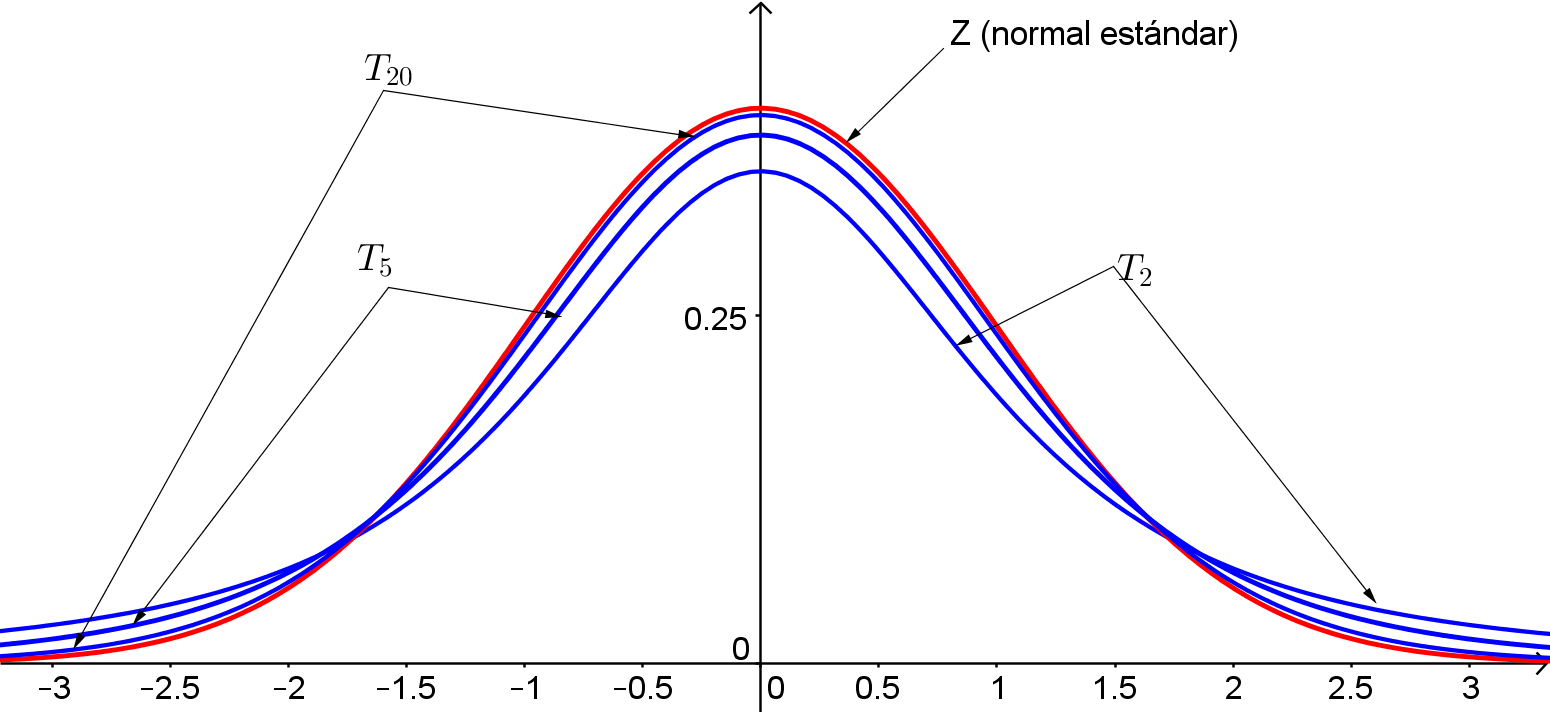
\includegraphics[width=13cm]{../fig/Cap06-ZvsT-figura.png}
\end{enColor}
\begin{bn}
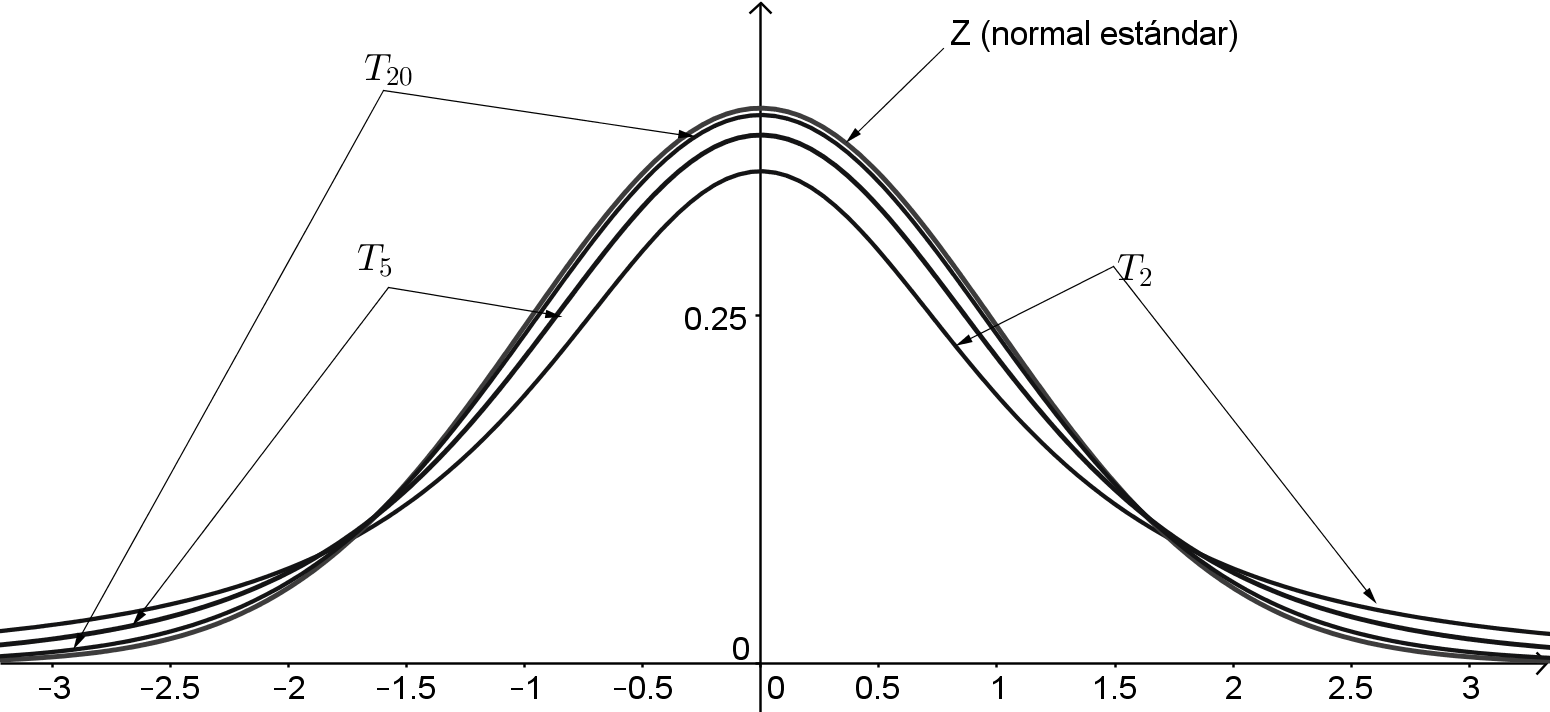
\includegraphics[width=13cm]{../fig/Cap06-ZvsT-figura-bn.png}
\end{bn}
\caption{La normal estándar $Z$, comparada con distribuciones $T_k$ de Student, para distintos valores de $k$.}
\label{cap06:fig:ZvsT}
\end{center}
\end{figure}

Como puede verse, no hay una única distribución $t$ de Student, sino toda una
familia de ellas, una para cada tamaño de la muestra. A pesar de esto, en
general seguiremos hablando de ``la'' $t$ de Student, como si fuera una sola.
Pues bien, la $t$ de Student, para cualquier valor de $k$, tiene una forma de
campana que recuerda a la normal, pero es más abierta. Se suele decir que la
$t$ de Student tiene colas más pesadas (que concentran más probabilidad) que
las de $Z$. A medida que el valor de $k$ aumenta, no obstante, la $t$ se parece
cada vez más a la normal estándar, de manera que para $k>30$ son esencialmente
iguales. Eso justifica que hayamos fijado $n>30$ como criterio para decidir si
una muestra es grande, a la hora de estimar $\mu_X$.

\subsection{Intervalos de confianza para $\mu$ con muestras pequeñas y varianza desconocida. Estadísticos.}
\label{cap06:subsec:IntConfMediaMuestraPequennaVarianzaDesconocida}

Vamos a explicar como usar la distribución $t$ de Student para construir un
intervalo de confianza para la media $\mu_X$, en el caso de $X$ normal, de tipo
$N(\mu_X,\sigma_X)$, cuando se dispone de una muestra pequeña ($n\leq 30$).
Queremos que el lector vea el paralelismo entre esta situación y la que ya
hemos visto en la Sección
\ref{cap06:sec:IntervaloConfianzaMediaPoblacionNormal}, así que vamos a
recordar el esquema de ideas que utilizamos en aquella sección. El punto de
partida era la segunda versión del Teorema Central del Límite, que aporta la
información necesaria sobre la distribución de la media muestral:
    \[\bar X \approx N\left(\mu_X,\dfrac{\sigma_X}{\sqrt{n}}\right).\]
Y aplicando la tipificación a esta relación, llegamos a $Z$:
    \begin{equation}\label{cap06:ecu:EstadisticoMediaMuestralconZ}
    Z=\dfrac{\bar X-\mu_X}{\dfrac{\sigma_X}{\sqrt{n}}},
    \end{equation}
Después nos dedicamos a (definir y) buscar el valor crítico $z_{\alpha/2}$ que
cumpliera:
    \[P\left(-z_{\alpha/2}<Z<z_{\alpha/2}\right)=\alpha\]
y, por el camino, gracias a la simetría de la distribución $Z$, vimos que esto
era lo mismo que pedir que fuera:
    \[P\left(Z\leq z_{\alpha/2}\right)=1-\dfrac{\alpha}{2}.\]
Pero una vez localizado, y calculado el valor crítico, basta con sustituir la
tipificación de $\bar X$ en la primera de estas dos ecuaciones de probabilidad
para obtener:
    \[P\left(-z_{\alpha/2}<\dfrac{\bar X-\mu_X}{\dfrac{\sigma_X}{\sqrt{n}}}
    <z_{\alpha/2}\right)=\alpha\]
Finalmente, despejando $\mu_X$ de las dos desigualdades interiores al
paréntesis, mediante una manipulación algebraica sencilla, llegamos al
intervalo de confianza:
    \[\bar X-z_{\alpha/2}\dfrac{\sigma_X}{\sqrt{n}}\leq \mu_X \leq \bar X+z_{\alpha/2}\dfrac{\sigma_X}{\sqrt{n}}.\]
Si se analizan los pasos de este esquema, queda patente que el paso clave es la
Ecuación \ref{cap06:ecu:EstadisticoMediaMuestralconZ}, porque es la que nos
permite relacionar los datos del problema con la normal estándar $Z$, que es
una variable aleatoria bien conocida, de la que tenemos mucha información, y
para la que podemos calcular los valores críticos, resolver problemas de
probabilidad, etc.

¿Qué ocurre en el caso de muestras pequeñas, que nos interesa ahora? Pues que,
gracias al trabajo de Student, tenemos la Ecuación \ref{cap06:ecu:DefinicionTStudent} (pág.
\pageref{cap06:ecu:DefinicionTStudent})
\[T_k=\dfrac{\bar X-\mu_X}{\dfrac{s}{\sqrt{n}}},\]
que nos permite relacionar los datos del problema con $T_k$, que es una
variable aleatoria bien conocida. de la que tenemos mucha información\ldots

El paralelismo es evidente,y nos conduce a un esquema prácticamente idéntico.
Buscaremos un valor crítico $t_{k;\alpha/2}$ que cumpla (luego daremos más
detalles sobre estos valores críticos):
    \[P\left(-t_{k;\alpha/2}< T_k <t_{k;\alpha/2}\right)=\alpha\]
Sustituimos aquí la Ecuación \ref{cap06:ecu:DefinicionTStudent},
    \[P\left(-t_{k;\alpha/2}< \dfrac{\bar X-\mu_X}{\dfrac{s}{\sqrt{n}}} <t_{k;\alpha/2}\right)=\alpha\]
Y de nuevo, despejando $\mu_X$ de las dos desigualdades interiores al
paréntesis, llegamos al intervalo de confianza:
    \[\bar X-t_{k;\alpha/2}\dfrac{s}{\sqrt{n}}\leq \mu_X \leq \bar X+t_{k;\alpha/2}\dfrac{s}{\sqrt{n}}.\]
El esquema funciona exactamente igual. Enseguida vamos a volver a estos
resultados, para hacerlos oficiales y aclarar los detalles que sean precisos
sobre los valores críticos de la $t$ de Student. Pero antes es casi más
importante insistir en que el lector trate de entender el esquema básico que
hemos usado, porque va a aparecer bastantes veces, con pequeñas variaciones, en
los próximos capítulos. El punto de partida siempre van a ser ecuaciones como
\label{cap06:lugar:ListaEstadisticosMedia}
\ref{cap06:ecu:EstadisticoMediaMuestralconZ}
\[Z=\dfrac{\bar X-\mu_X}{\dfrac{\sigma_X}{\sqrt{n}}},\]
o como \ref{cap06:ecu:EstadisticoMediaMuestralSigmaDesconocidaMuestraGrande},
con $s$ en lugar de $\sigma$, para muestras grandes (pág.
\pageref{cap06:ecu:EstadisticoMediaMuestralSigmaDesconocidaMuestraGrande}),
\[Z=\dfrac{\bar X-\mu_X}{\dfrac{s}{\sqrt{n}}},\]
o  como \ref{cap06:ecu:DefinicionTStudent}:
\[T_k=\dfrac{\bar X-\mu_X}{\dfrac{s}{\sqrt{n}}}.\]
La cantidad que aparece en el miembro derecho de ambas ecuaciones es lo que
vamos a llamar un {\sf estadístico}. De hecho, en el próximo capítulo, lo
llamaremos (de forma más completa) un {\sf estadístico de
contraste}\index{estadístico de contraste} (en inglés, {\em test
statistic}\index{test statistic}). El estadístico, como puede verse, no es ni un
parámetro de la población como $\mu$ o $\sigma$, ni un estimador como $\bar X$
o $s$, sino que muchas veces es una variable aleatoria que mezcla ambos tipos de objetos y que tiene
una propiedad fundamental: su distribución de probabilidad no depende del
problema concreto en el que andamos trabajando, y es una de las {\em
distribuciones clásicas}, de esas distribuciones con nombre y apellidos, como
$Z$ o la $t$ de Student. De esa forma, el servicio que nos presta el
estadístico es que nos permite traducir los datos de nuestro problema a las
distribuciones clásicas, que juegan el papel de {\em escalas universales de
probabilidad}, para las que disponemos de mucha información.

Para resumir los resultados de este apartado, en lo que se refiere al problema
de estimar $\mu_X$ en poblaciones normales, usando muestras pequeñas, empezamos
por definir los valores críticos de la distribución $t$.

    \begin{center}
    \fcolorbox{black}{Gris025}{
    \begin{minipage}{12.5cm}
        \begin{center}
        %%%%%%%%%%%%%%%%%%%%%%%%%%%%%%%%%%%%%%%
        {\bf  Valores críticos $t_{k;\alpha/2}$ de distribución $t$ de Student.}\\
        \end{center}
        \index{valores críticos de la $t$ de Student}
        \index{$t_{k;p}$, $t_{k;\alpha}$ valor crítico de $t$}
       %%%%%%%%%%%%%%%%%%%%%%%%%%%%%%%%%%%%%%%
       Sea $0\leq p\leq 1$ un valor de probabilidad cualquiera, y sea $k$ un número natural. El {\sf valor crítico} de la distribución $t$ de Student con $k$  grados de libertad, correspondiente a $p$ es el valor $t_{k;p}$ que cumple:
       \begin{equation}\label{cap06:ecu:DefinicionValorCriticoT}
       P(T_k\leq t_{k;p})=1-p.
       \end{equation}
        Gráficamente, $t_{k;p}$ es el valor que deja una probabilidad $p$ en su cola derecha (es decir, $1-p$ en la cola izda.) Ver la Figura \ref{cap06:fig:ValorCriticoT}.
       %%%%%%%%%%%%%%%%%%%%%%%%%%%%%%%%%%%%%%%
    \end{minipage}}
    \end{center}
En el Tutorial06 veremos como usar el ordenador para resolver problemas directos e
inversos de probabilidad que involucren a la $t$ de Student. Y, desde luego,
aprenderemos a calcular los valores críticos de $t$.

\begin{figure}[h!]
\begin{center}
\begin{enColor}
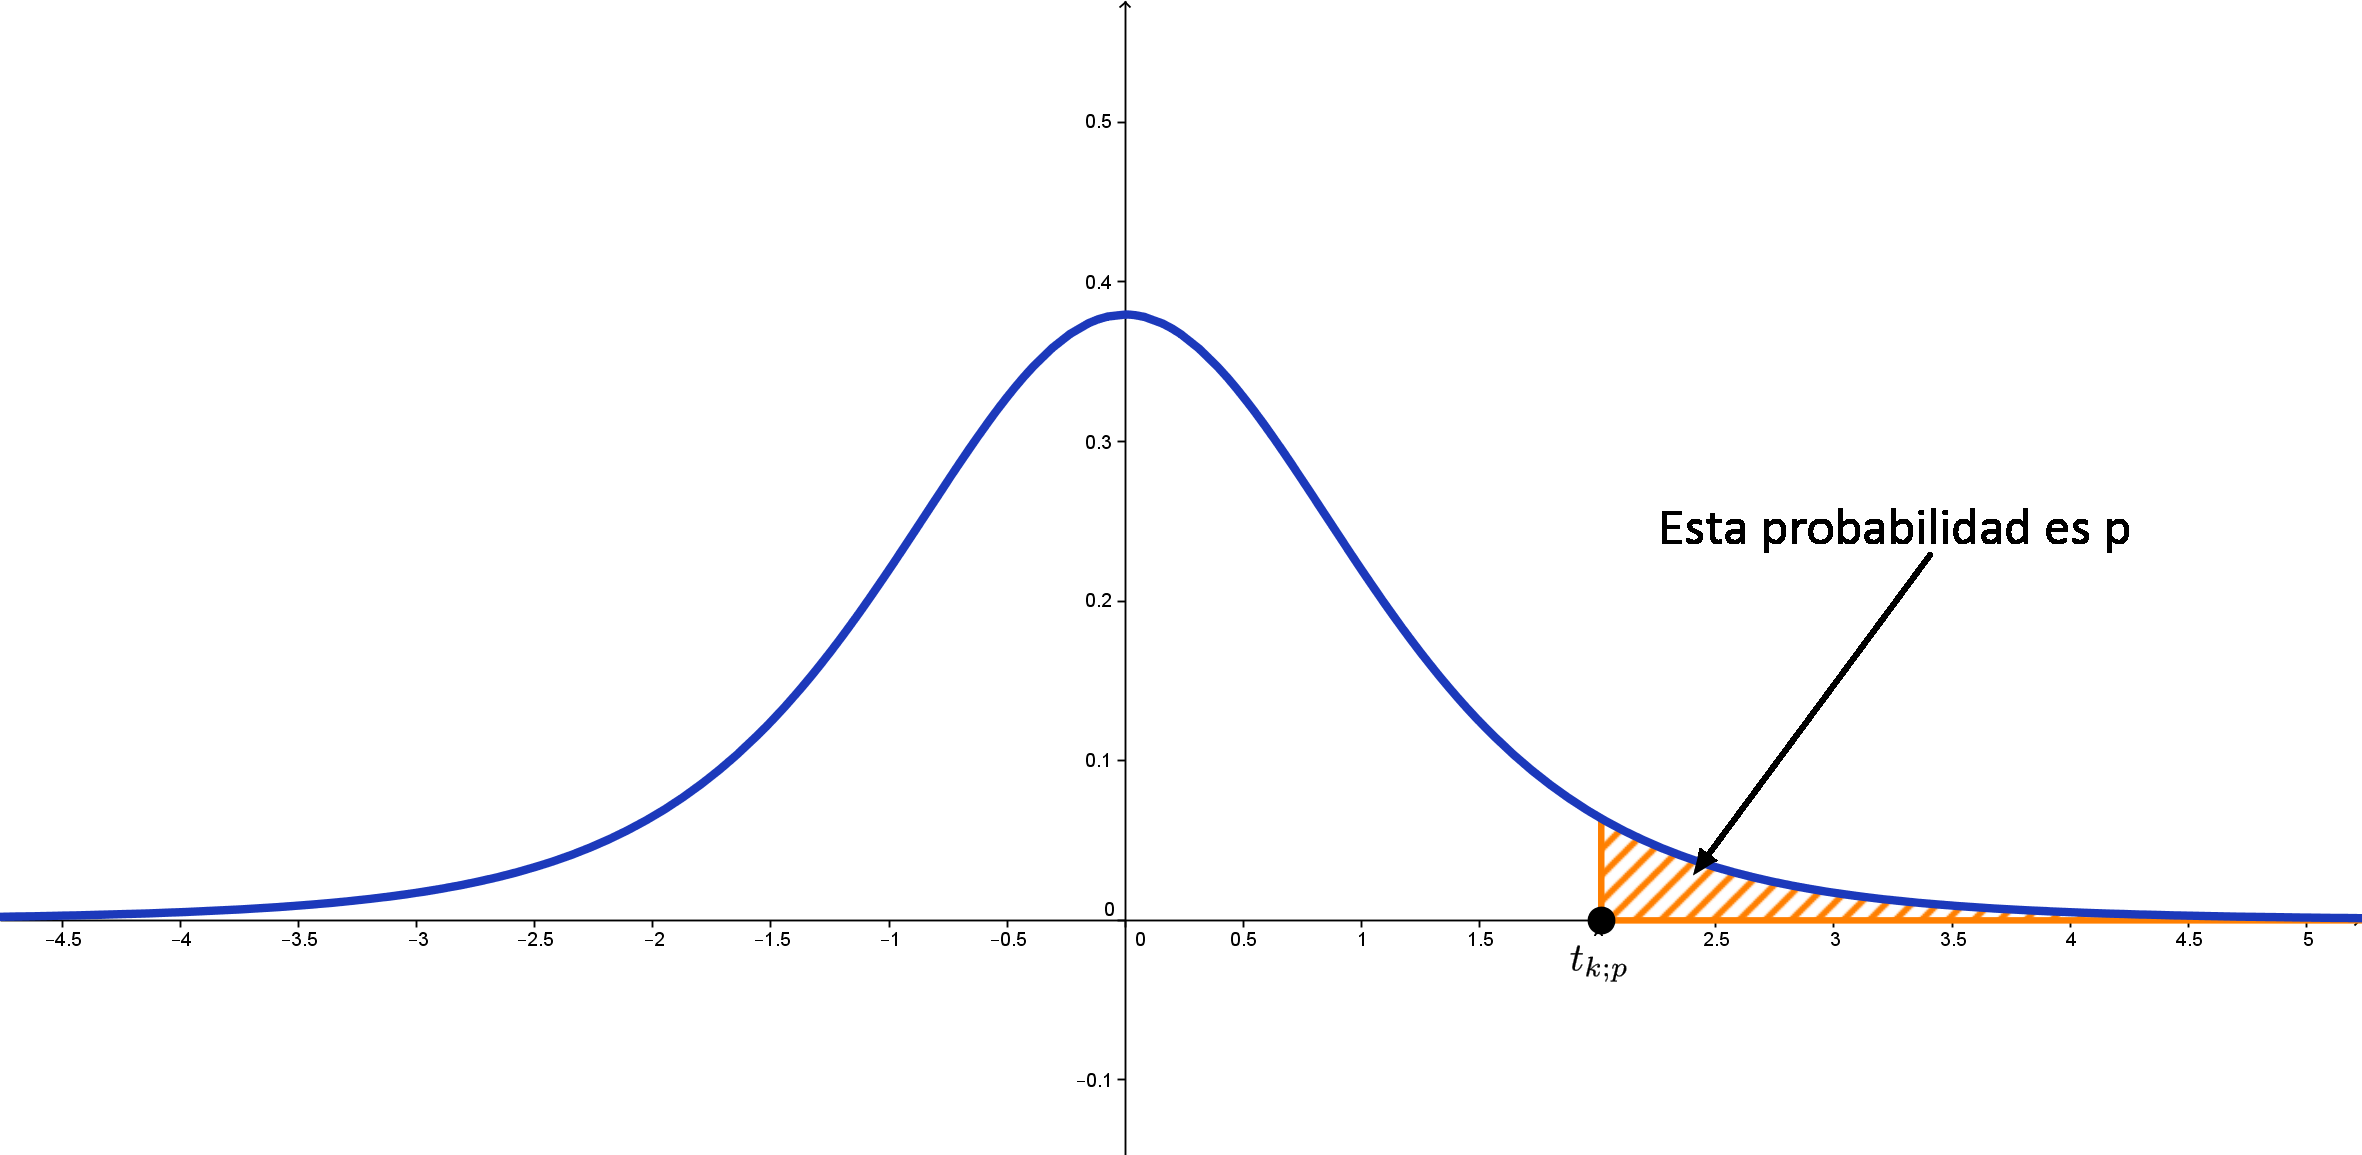
\includegraphics[width=13cm]{../fig/Cap06-ValoresCriticosT.png}
\end{enColor}
\begin{bn}
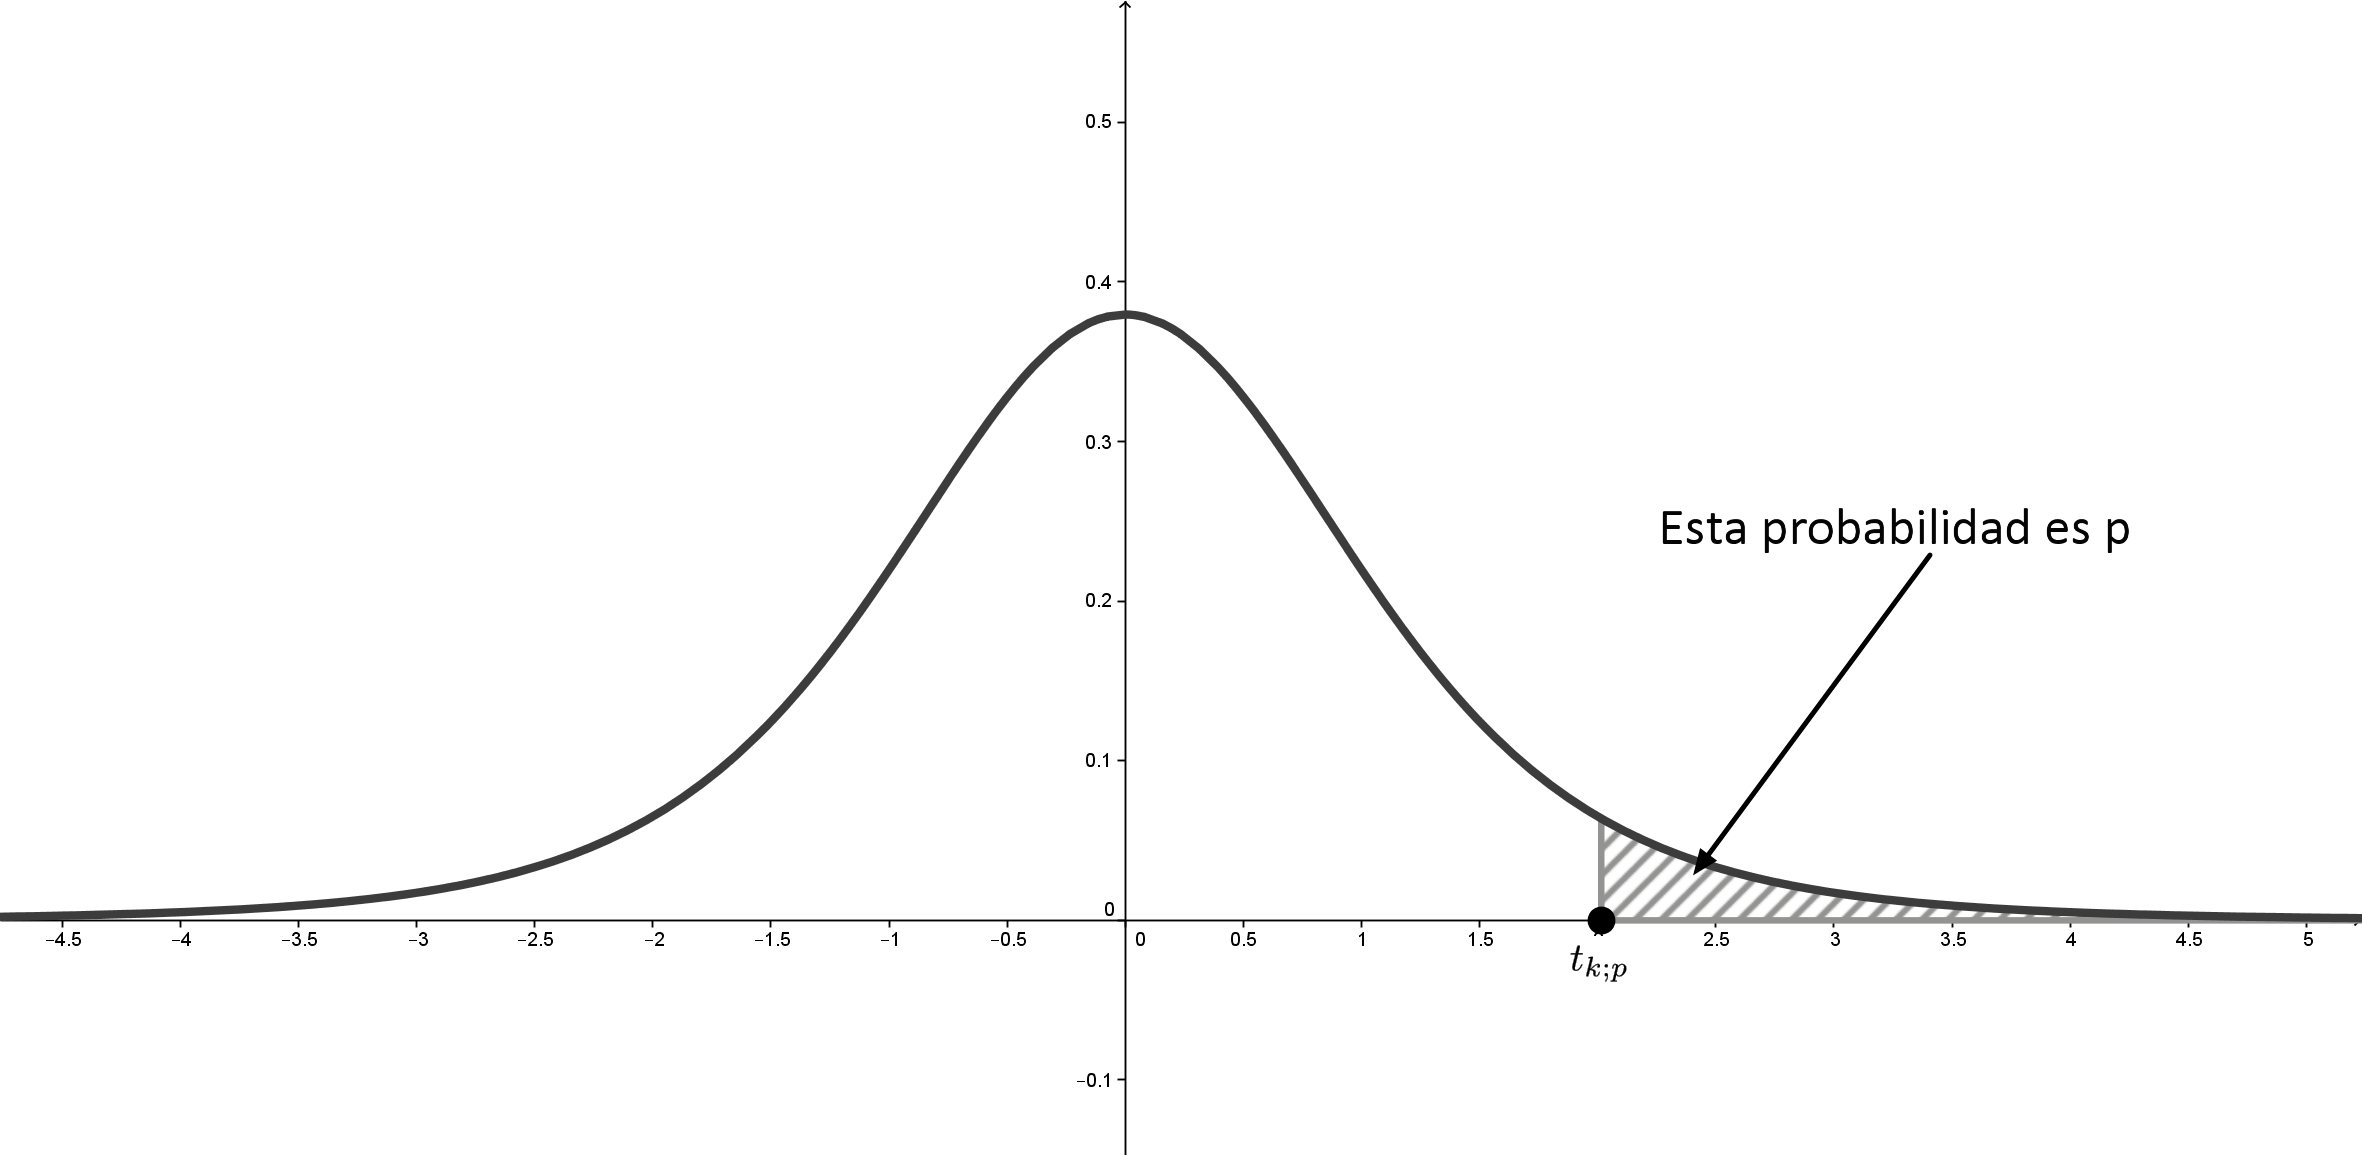
\includegraphics[width=13cm]{../fig/Cap06-ValoresCriticosT-bn.png}
\end{bn}
\caption{El valor crítico $t_{k;p}$ de la distribución $T_k$ de Student.}
\label{cap06:fig:ValorCriticoT}
\end{center}
\end{figure}

El valor crítico $t_{k;\alpha/2}$ en particular, es el que necesitamos para el
intervalo de confianza para la media. Este valor satisface:
    \[P\left(T_k\leq t_{k;\alpha/2}\right)=1-\dfrac{\alpha}{2},\]
y, por lo tanto, deja en su cola derecha una probabilidad igual a
$\dfrac{\alpha}{2}$. Con el cálculo de este valor tendremos todo lo necesario
para completar el cálculo del intervalo de confianza, que ahora hacemos
oficial.

    \begin{center}
    \fcolorbox{black}{Gris025}{
    \begin{minipage}{12.5cm}
        \begin{center}
        %%%%%%%%%%%%%%%%%%%%%%%%%%%%%%%%%%%%%%%
       {\bf Intervalo de confianza para la media $\mu$ usando $t$ de Student.}\\[3mm]
       {\bf Población normal, varianza desconocida, muestras pequeñas $n<30$.}\\
       \index{intervalo de confianza para la media usando $t$}
        \end{center}
       %%%%%%%%%%%%%%%%%%%%%%%%%%%%%%%%%%%%%%%
       Sea $X$ una variable aleatoria normal, Si consideramos muestras de tamaño $n$, y por lo tanto el número de grados de libertad es $k=n-1$, entonces un intervalo de confianza al nivel $(1-\alpha)$  para la media $\mu_X$ es:
       \begin{equation}\label{cap06:ecu:IntervaloConfianzaMediaUsandoT}
       \bar X-\colorbox{lightgrey}{$t_{k;\alpha/2}$}\dfrac{s}{\sqrt{n}}\leq \mu_X \leq \bar X+\colorbox{lightgrey}{$t_{k;\alpha/2}$}\dfrac{s}{\sqrt{n}}.
       \end{equation}
       que también escribiremos:
       \[\mu_X =\bar X \pm \colorbox{lightgrey}{$t_{k;\alpha/2}$}\dfrac{s}{\sqrt{n}}.\]
       %%%%%%%%%%%%%%%%%%%%%%%%%%%%%%%%%%%%%%%
    \end{minipage}}
    \end{center}
Para construir el intervalo de confianza para $\mu$, en el caso de muestras
grandes con $n>30$, se puede utilizar tanto la normal estándar $Z$  (Ecuación
\ref{cap06:ecu:IntervaloConfianzaMediaMuestraGrande}) como la $t$ de Student
(la Ecuación \ref{cap06:ecu:IntervaloConfianzaMediaUsandoT} que acabamos de
ver). ¿Cuál es preferible? No hay grandes diferencias en ese caso, pero si
tenemos en cuenta que las colas de la $t$ de Student son algo más pesadas, el
intervalo que se obtiene usando $t$ será siempre ligeramente más ancho que el
de $Z$, y por ello, ligeramente menos preciso.


Veamos un ejemplo de construcción de un intervalo de confianza, usando la $t$
de Student:
\begin{ejemplo}
\label{cap06:ejem:IntConfMediaConTBacterias}
    Una muestra de 10 bacterias Vibrio cholerae tiene una longitud media de $\bar X=2.35\mu$m y una
    cuasidesviación típica $s=0.61\mu$m. Hallar intervalos de confianza al $95\%$ y al $99\%$ para
    la longitud de estas
    bacterias.\\[3mm]


    Puesto que $n=10$, usamos la distribución $t$ y tomamos $k=9$ grados de libertad. Al nivel $1-\alpha=0.95$ (es decir, $\alpha/2=0.025$) Calculamos
    \[t_{9;0.025}\approx 2.26\]
    %corrección hecha por mi
    El intervalo al $95\%$ es:
    \[\bar X \pm \textcolor{black}{\mbox{$t_{k;\alpha/2}$}}\dfrac{s}{\sqrt{n}}=2.35\pm 2.26\cdot\dfrac{0.61}{\sqrt{10}}=2.35\pm 0.44 = (1.91, 2.79).\]
    Para el intervalo al $99\%$ calculamos:
    \[t_{9;0.005}\approx 3.25\]
    %corrección hecha por mi
    y se obtiene:
    \[\bar X \pm \textcolor{black}{\mbox{$t_{k;\alpha/2}$}}\dfrac{s}{\sqrt{n}}=2.35\pm 3.25\cdot\dfrac{0.61}{\sqrt{10}}=2.35\pm 0.63=(1.72,2.98),\]
    naturalmente más ancho que el anterior.\qed
\end{ejemplo}

No queremos cerrar el tema de los intervalos de confianza para la media, sin
recordar al lector que hay un caso en el que los métodos de este capítulo no
proporcionan una respuesta: si la muestra es pequeña, y la variable $X$ no es
normal (o no tenemos razones para suponer que lo sea), entonces no podemos
aplicar ninguna de las fórmulas de este capítulo para obtener un intervalo de
confianza para $\mu_X$. En ese caso se necesitan métodos {\em no paramétricos},
más avanzados.

\section{Inferencia sobre la varianza. Distribución $\chi^2$.}
\label{cap06:sec:InferenciaVarianzaDistribucionChi2}

En las secciones previas hemos tratado el problema de la estimación de $\mu_X$,
la media de la población. Pero si, como sucede a menudo, la población es
normal, de tipo $N(\mu_X,\sigma_X)$, entonces su distribución no queda
completamente caracterizada hasta que hayamos estimado también la varianza
$\sigma^2_X$ (y, con ella, la desviación típica). Ese es el problema del que
nos vamos a ocupar en esta, la última sección del capítulo.

Centremos por tanto nuestra atención en una variable $X$ de tipo
$N(\mu,\sigma)$ (como no hay riesgo de confusión, no usaremos el subíndice $X$,
así que en esta sección $\mu=\mu_X$ y $\sigma=\sigma_X$).  ¿Cuál es el
candidato natural para estimar $\sigma^2$ a partir de una muestra? En realidad,
ya hemos discutido esto en la Sección \ref{cap06:sec:DesviacionTipicaMuestral},
y allí llegamos a la conclusión de que el estimador insesgado natural era
$s^2$, la cuasivarianza muestral definida por:
       \[s^2=\dfrac{\displaystyle\sum_{i=1}^n(x_i-\bar x)^2}{n-1}.\]
Atención: el denominador es $n-1$. Para empezar, vamos a intentar evitar una
posible confusión, que puede resultar del trabajo en secciones previas. Hasta
ahora, hemos usado $s^2$ como una herramienta auxiliar, {\em con el objetivo de
estimar $\mu$ mediante $\bar X$}. El protagonista de aquella estimación, por
así decirlo, era $\bar X$, como estimador de $\mu$. Pero ahora queremos centrar
nuestra atención en $s^2$, sin nadie que le robe protagonismo, y preguntarnos
¿cómo se puede usar $s^2$ {\em para estimar $\sigma^2$}, la varianza
poblacional?

Cuando hicimos la estimación de $\mu$, empezamos por el Teorema Central del
Límite, que nos proporcionó la información que necesitábamos sobre la
distribución del estadístico
\[\dfrac{\bar X-\mu_X}{\dfrac{s}{\sqrt{n}}}.\]
Ahora debemos hacer lo mismo. Tenemos que obtener algún resultado sobre la
distribución de $s^2$ en las muestras. Sea por lo tanto $X$ una variable
aleatoria con distribución de tipo $N(\mu,\sigma)$ (que representa a la
población), y sea $X_1,X_2,\ldots,X_n$ una muestra aleatoria de $X$ (como
siempre, las $X_i$ son $n$ copias independientes de $X$).  Entonces:
    \[s^2=\dfrac{\displaystyle\sum_{i=1}^n(X_i-\bar X)^2}{{n-1}}.\]
(La diferencia -sutil- entre esta expresión y la anterior, es que allí los
$x_i$ son números, y aquí $X_i$ son variables aleatorias; no te preocupes si,
al principio, no lo ves claro). Como siempre, vamos a tratar de relacionar esto
con la normal estándar $N(0,1)$. Para conseguirlo, vamos a dividir esta
expresión por $\sigma^2$, y la reorganizaremos, con la idea de tipificación
como guía:
    \begin{equation}\label{cap06:ecu:ObtenerDistribucionCuasivarianzaMuestral}
        \dfrac{s^2}{\sigma^2}=\dfrac{\displaystyle\sum_{i=1}^n(X_i-\bar X)^2}{\sigma^2\cdot(n-1)}=
        \dfrac{1}{(n-1)}\dfrac{\displaystyle\sum_{i=1}^n(X_i-\bar X)^2}{\sigma^2}=\dfrac{1}{(n-1)}\sum_{i=1}^n\left(\dfrac{(X_i-\bar X)^2}{\sigma^2}\right)=
    \end{equation}
    \[
        =\colorbox{lightgrey}{$\dfrac{1}{(n-1)}\sum_{i=1}^n\left(\dfrac{X_i-\bar X}{\sigma}\right)^2$}=\dfrac{1}{(n-1)}\sum_{i=1}^n Z_i^2=\dfrac{1}{n-1}(Z_1^2+Z_2^2+\cdots+Z_n^2).\]
Hemos destacado, sombreándolo, el paso en el que tipificamos las $X_i$, y
obtenemos las $Z_i$ que son, cada una de ellas, copias de la normal estándar.

Lo que hace que esta situación sea más complicada es que las $Z_i$ están
elevadas al cuadrado. Si, en lugar de esto, tuviéramos
    \[\dfrac{1}{n-1}(Z_1+Z_2+\cdots+Z_n),\]
podríamos decir que la suma de las normales es una normal (con media $0$ y
varianza igual a $n$, aunque eso aquí no importa). Pero no es así: cada $Z_i$
aparece elevada al cuadrado, {\em y el cuadrado de una variable con
distribución normal, no es, no puede ser, una variable con distribución
normal}. Esto es relativamente fácil de entender: la normal estándar $Z$ toma
valores positivos y negativos, como de hecho sucede con cualquier otra normal.
Pero en cuanto la elevamos al cuadrado, deja de tomar valores negativos. Así
que, como decíamos, el cuadrado de una normal estándar no puede ser una normal,
y la suma de unos cuantos cuadrados de normales estándar tampoco resulta ser
una normal (ni estándar, ni no estándar, simplemente no es normal).


Parece que estamos en un atolladero. Pero sólo si nos empeñamos en seguir
buscando la normal. Si la dificultad es que tenemos una suma de copias
independientes de $Z^2$, habrá que preguntarse ¿qué tipo de variable aleatoria
es esa suma? La respuesta es otra de las distribuciones más importantes de la
Estadística.

    \begin{center}
    \fcolorbox{black}{Gris025}{
    \begin{minipage}{12.5cm}
        \begin{center}
        %%%%%%%%%%%%%%%%%%%%%%%%%%%%%%%%%%%%%%%
        {\bf  Distribución $\chi^2$. Media y varianza.}\\
        \end{center}
        \index{distribución $\chi^2$}
        \index{$\chi^2$}
       %%%%%%%%%%%%%%%%%%%%%%%%%%%%%%%%%%%%%%%
       Si la variable aleatoria $Y$ es la suma de los cuadrados de una familia de $n$ copias independientes de la distribución normal estándar, entonces diremos que $Y$ es de {\sf tipo $\chi^2_k$}, con $k=n-1$ grados de libertad.\\
       La media de $\chi^2_k$ es $\mu_{\chi^2_k}=k$, y su desviación típica es $\sigma_{\chi^2_k}=\sqrt{2k}$.
       %%%%%%%%%%%%%%%%%%%%%%%%%%%%%%%%%%%%%%%
    \end{minipage}}
    \end{center}

%\pendiente{(de \link{http://en.wikipedia.org/wiki/Karl_Pearson}{Pearson})}

La experiencia con la normal y la $t$ de Student nos ha enseñado que una de las
mejores formas de familiarizarse con una distribución continua es mediante la
gráfica de su función de densidad. En el caso de la $\chi^2$, su función de
densidad (para $k=4$) tiene el aspecto de la  Figura
\ref{cap06:fig:DensidadChiCuadrado} (atención a las escalas de los ejes). Ese
es el aspecto típico para los primeros valores $k>1$. El caso $k=1$ es
especial, y para valores grandes de $k$ se obtiene una forma más acampanada. En el Tutorial06 veremos de forma dinámica como cambia la forma de esta distribución cuando cambiamos el valor de $k$.
%El fichero GeoGebra
%\fichero{../datos/Cap06-DensidadChiCuadrado.html}{Cap06-DensidadChiCuadrado.html}
%permite observar esto con más claridad.

\begin{figure}[htb]
\begin{center}
\begin{enColor}
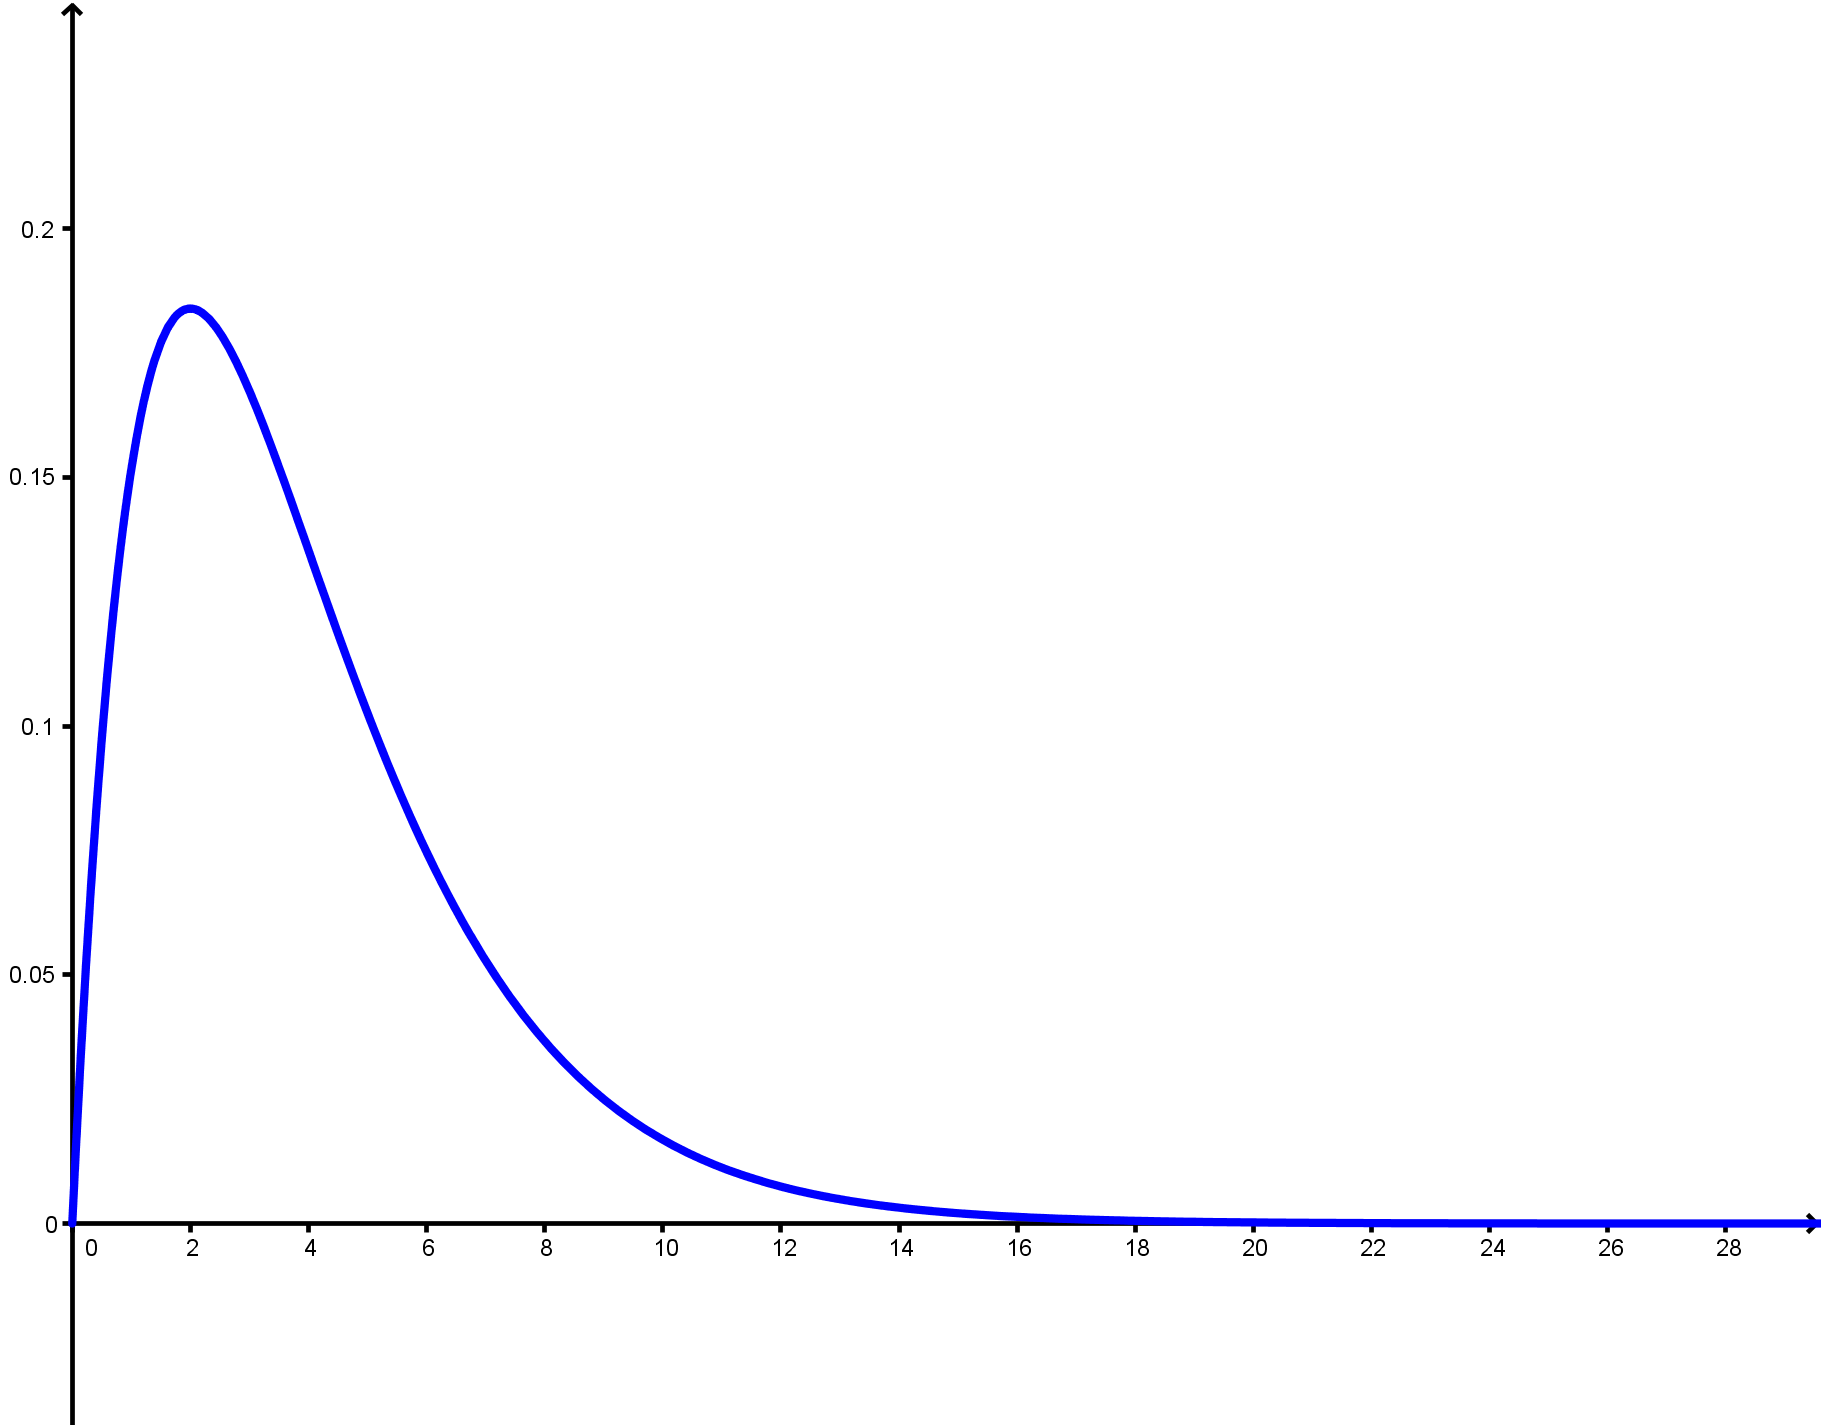
\includegraphics[width=12.5cm]{../fig/Cap06-DensidadChiCuadrado.png}
\end{enColor}
\begin{bn}
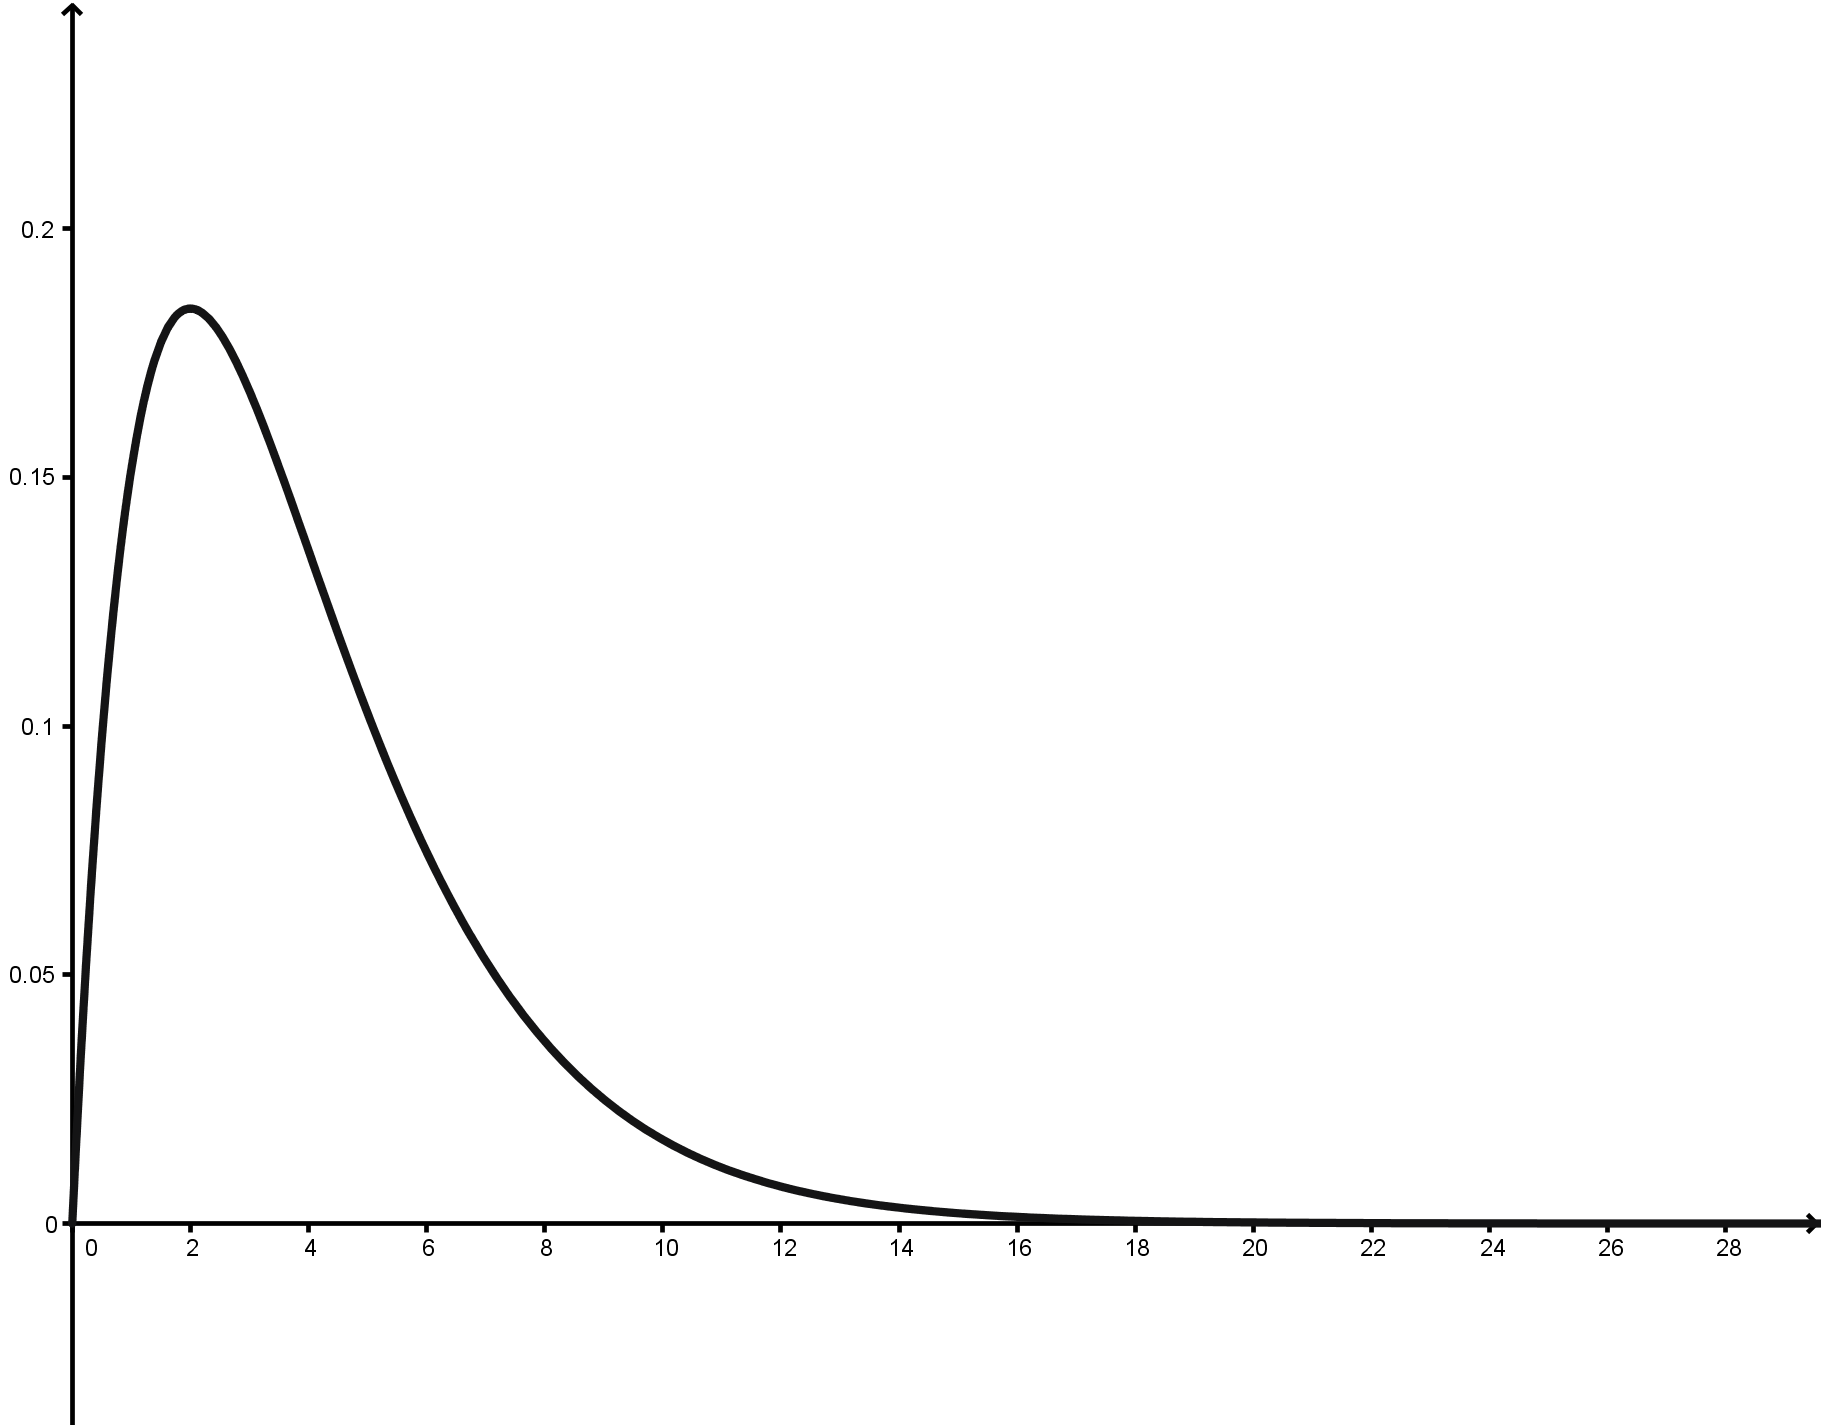
\includegraphics[width=12.5cm]{../fig/Cap06-DensidadChiCuadrado-bn.png}
\end{bn}
\caption{Función de densidad de la distribución $\chi^2$ con $k=4$ grados de libertad.}
\label{cap06:fig:DensidadChiCuadrado}
\end{center}
\end{figure}

Observa, en esa figura, que la función sólo está definida a la
derecha del $0$ (no hay probabilidad asociada para los valores negativos. Y,
desde luego, no hay nada ``simétrico'' en esta distribución, en el sentido en
el que la cola izquierda y la derecha de la normal eran simétricas. La fórmula
de esta función de densidad es:
         \[f(x;n)=
         \begin{cases}
         \dfrac{1}{2^{k/2}\Gamma(k/2)}x^{(k/2)-1}e^{-x/2}&\mbox{ si }x\geq 0\\
         0&\mbox{ si }x<0
         \end{cases}
         \]
donde $\Gamma$ es la denominada {\sf función Gamma}. Puedes encontrar más información sobre esta función en el libro \cite{garcia2009estadistica} (o en el enlace [\,\ref{enlace0012}\,]\label{enlace0012a}) de la Wikipedia). Como en el caso de la $t$ de Student, no es necesario, ni mucho menos, que te aprendas esta
fórmula. Sólo la incluimos como referencia, pero cuando tengamos que calcular algún valor,
acudiremos al ordenador. En el Tutorial06 veremos en detalle como hacerlo.
%Podemos adelantar que, en R, las funciones adecuadas son {\tt pchisq} (para problemas directos, en
%los que calculamos {\em {\tt p}robabilidades}) y {\tt qchisq} (para problemas inversos, cuando
%calculamos {\em {\tt q}uantiles}).

\subsubsection{Cuantiles de la distribución $\chi^2$ ({!`}qué no es simétrica!)}\label{cap07:subsubsec:ChiCudadradoNoEsSimetrica}

El hecho de que la distribución $\chi^2$ no sea simétrica supone una diferencia
importante, al trabajar con ella, comparada con lo que sucedía con $Z$ o la $t$
de Student. En esas dos distribuciones, la cola izquierda y derecha eran
siempre simétricas. Eso se traducía, por ejemplo, en que para cualquier valor
de probabilidad $p_0$
\[z_{p_0}=-z_{1-p_0}.\]
porque $z_{p_0}$ es el valor que deja una probabilidad igual a $p_0$ a su
derecha, y $z_{1-p_0}$ es el que deja una probabilidad igual a $p_0$ a su
izquierda. Y, a su vez, esto nos ha permitido escribir fórmulas como esta para
los intervalos de confianza (ver pág.
\pageref{cap06:ecu:IntervaloConfianzaMediaMuestraGrande}):
\[\mu_X =\bar X \pm z_{\alpha/2}\dfrac{s}{\sqrt{n}}.\]
usando el mismo cuantil para los extremos izquierdo y derecho del intervalo. El
intervalo de confianza, en estos casos, está centrado en $\bar X$.

Todas estas propiedades se pierden cuando la distribución deja de ser
simétrica, como sucede con $\chi^2$. Vamos a pensar en los problemas inversos,
para intentar dejar esto más claro.

\begin{ejemplo}
\label{cap06:ejem:ProblemaDirectoInversoProbabilidadChi}

Supongamos que, usando la distribución
$\chi^2_4$, queremos localizar el valor $a$ que deja, en su cola  izquierda,
una probabilidad igual a $0.05$. Este problema se ilustra en la Figura
\ref{cap06:fig:ChiCuadradoProblemaInversoIzquierda}. El valor que se obtiene
%(por ejemplo, con R, usando {\tt qchisq(0.05,df=4)})
usando el ordenador es $\approx 0.7107$.

\begin{figure}[htb]
\begin{center}
\begin{enColor}
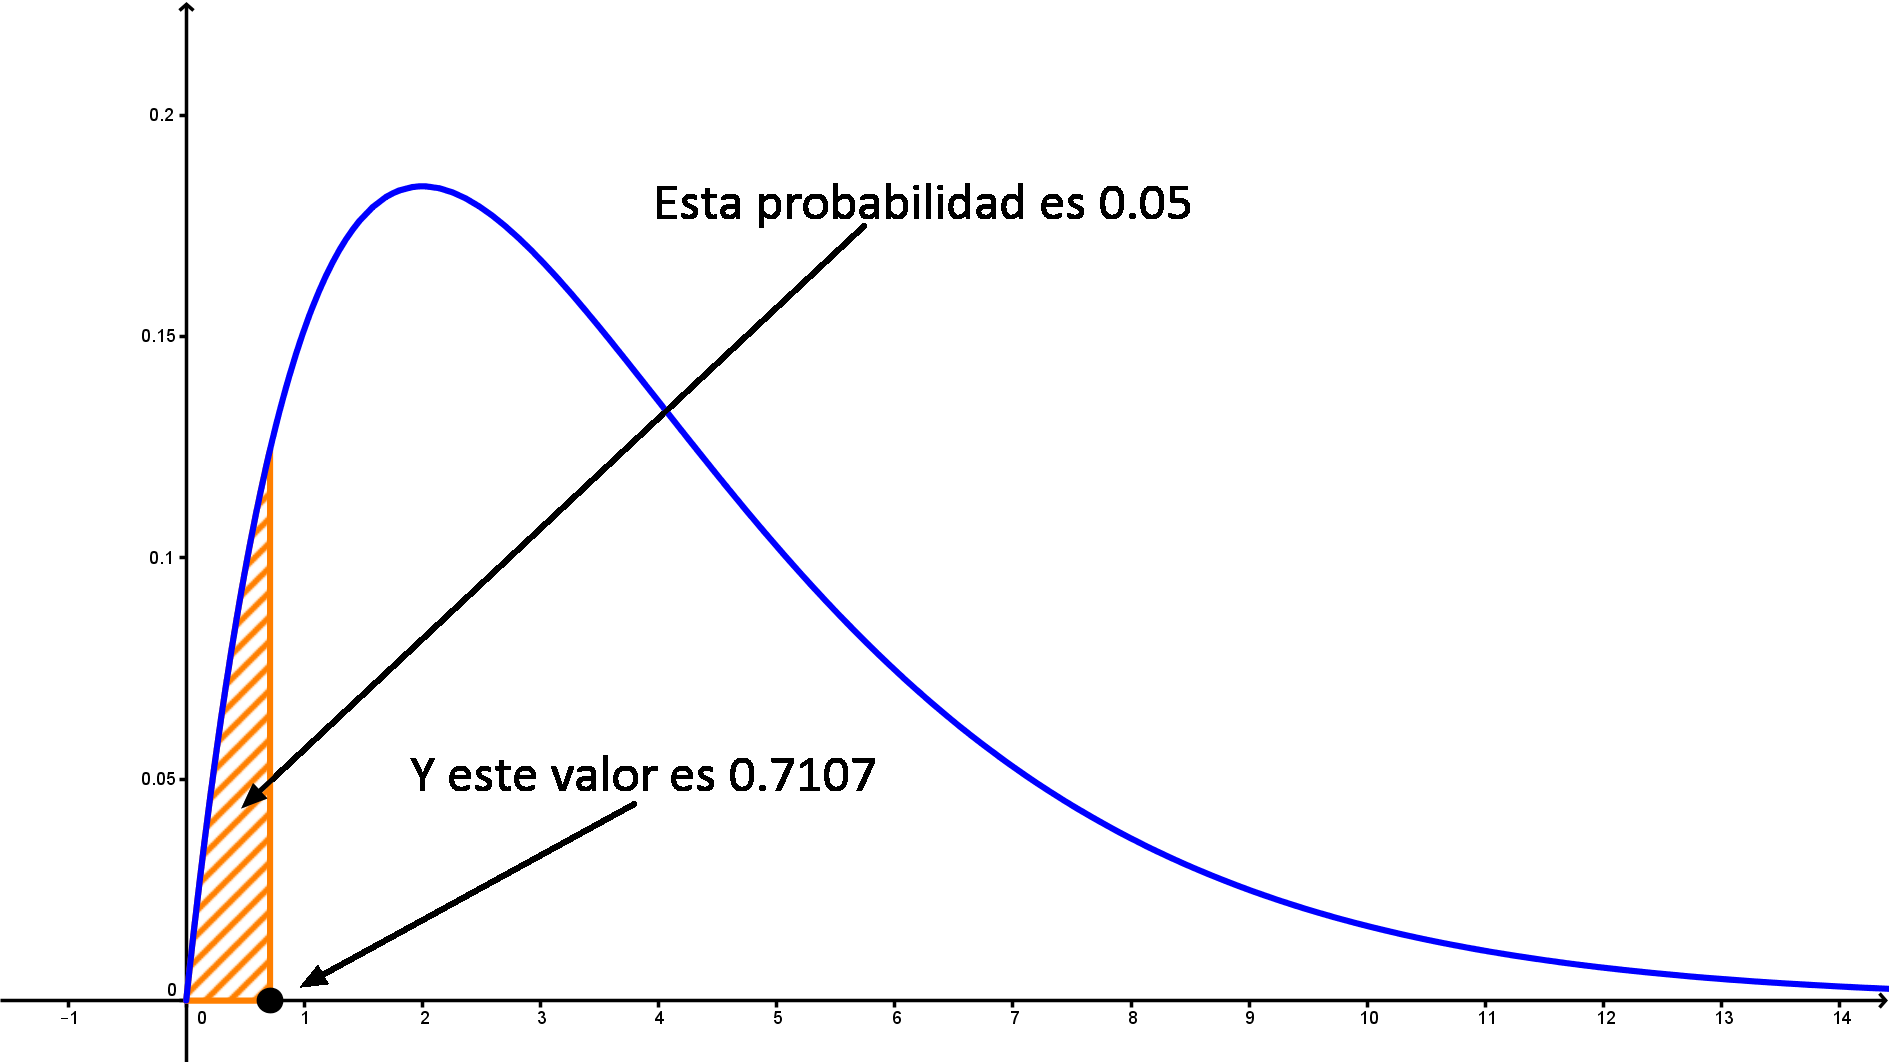
\includegraphics[width=13cm]{../fig/Cap06-ChiCuadradoProblemaInversoIzquierda.png}
\end{enColor}
\begin{bn}
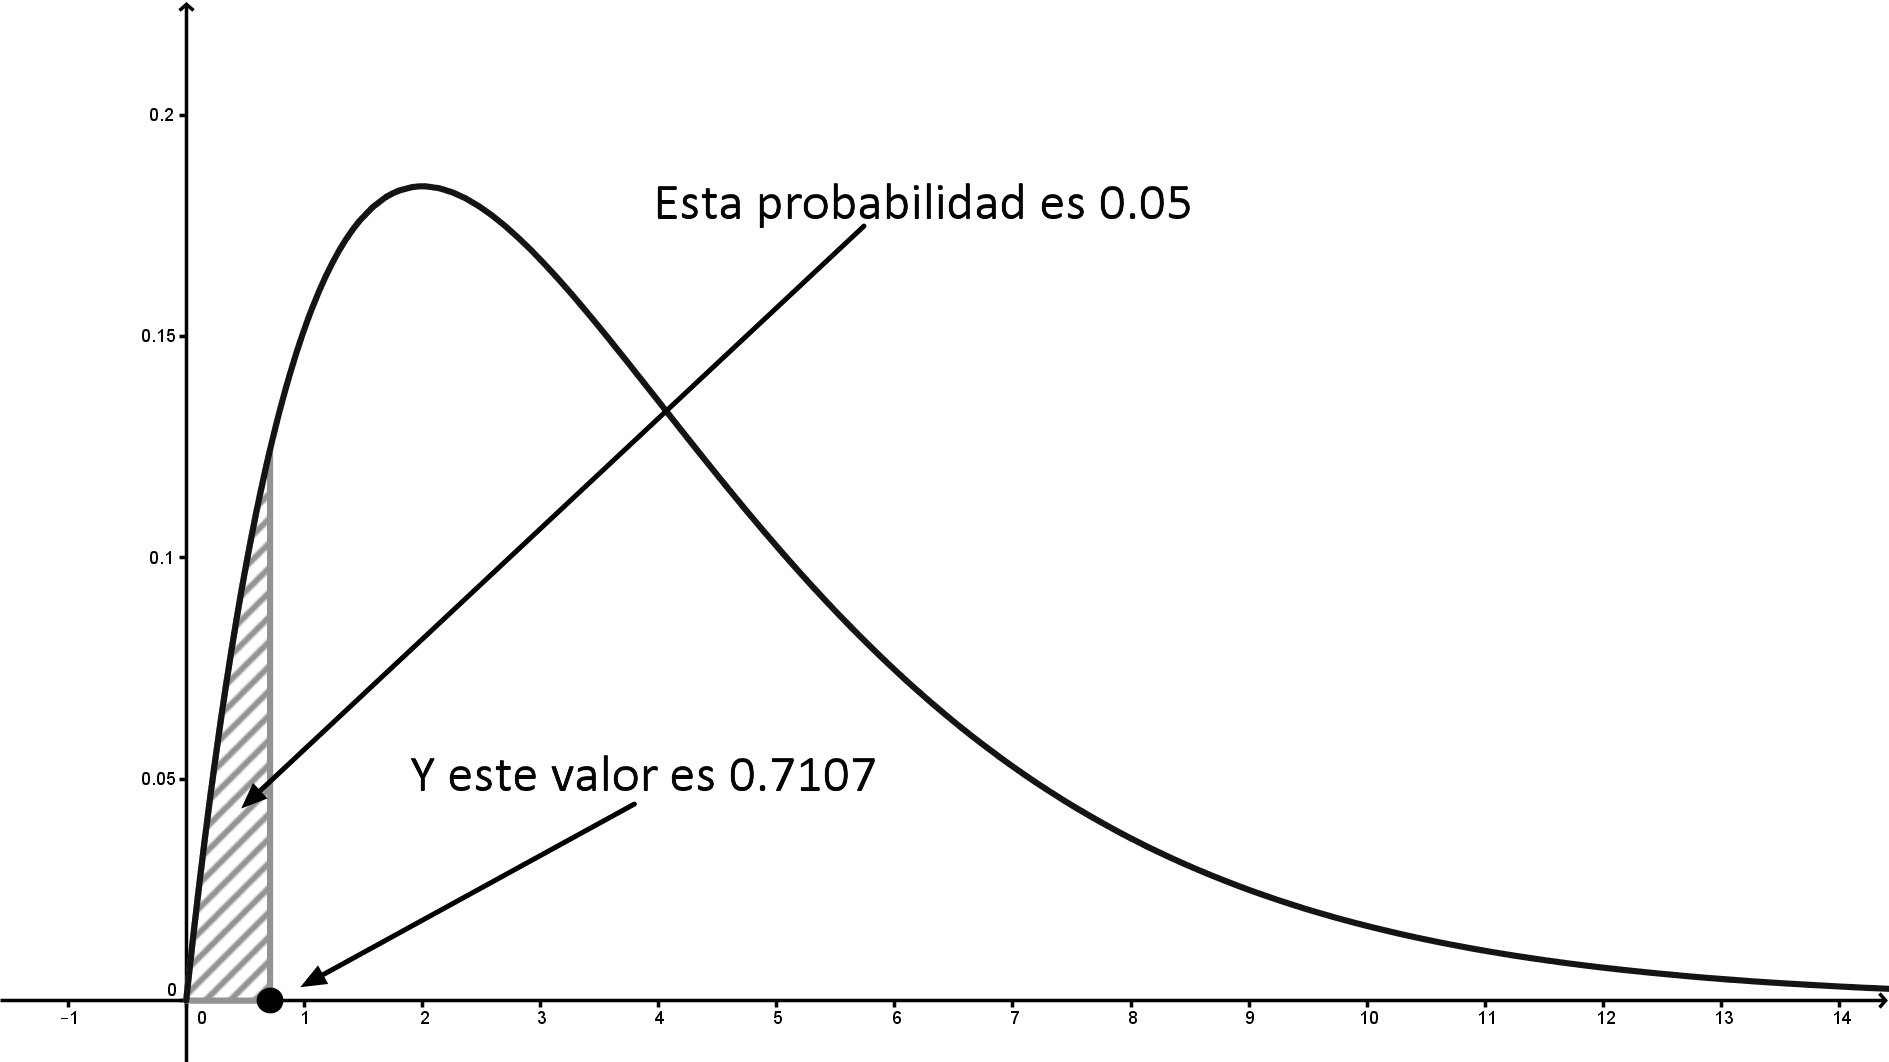
\includegraphics[width=13cm]{../fig/Cap06-ChiCuadradoProblemaInversoIzquierda-bn.png}
\end{bn}
\caption{Problema inverso de probabilidad ($p_0=0.05$) para $\chi^2_4$, cola izquierda.}
\label{cap06:fig:ChiCuadradoProblemaInversoIzquierda}
\end{center}
\end{figure}

De forma similar, y usando también $\chi^2_4$, podemos plantear la pregunta de
cuál es el valor que deja, en su cola derecha, la misma probabilidad $0.05$.
Este problema se ilustra en la Figura
\ref{cap06:fig:ChiCuadradoProblemaInversoDerecha}. El valor que proporciona el ordenador
%(por ejemplo, con R, usando {\tt qchisq(0.05,df=4)})
es $\approx 9.488$. \qed

\begin{figure}[htb]
\begin{center}
\begin{enColor}
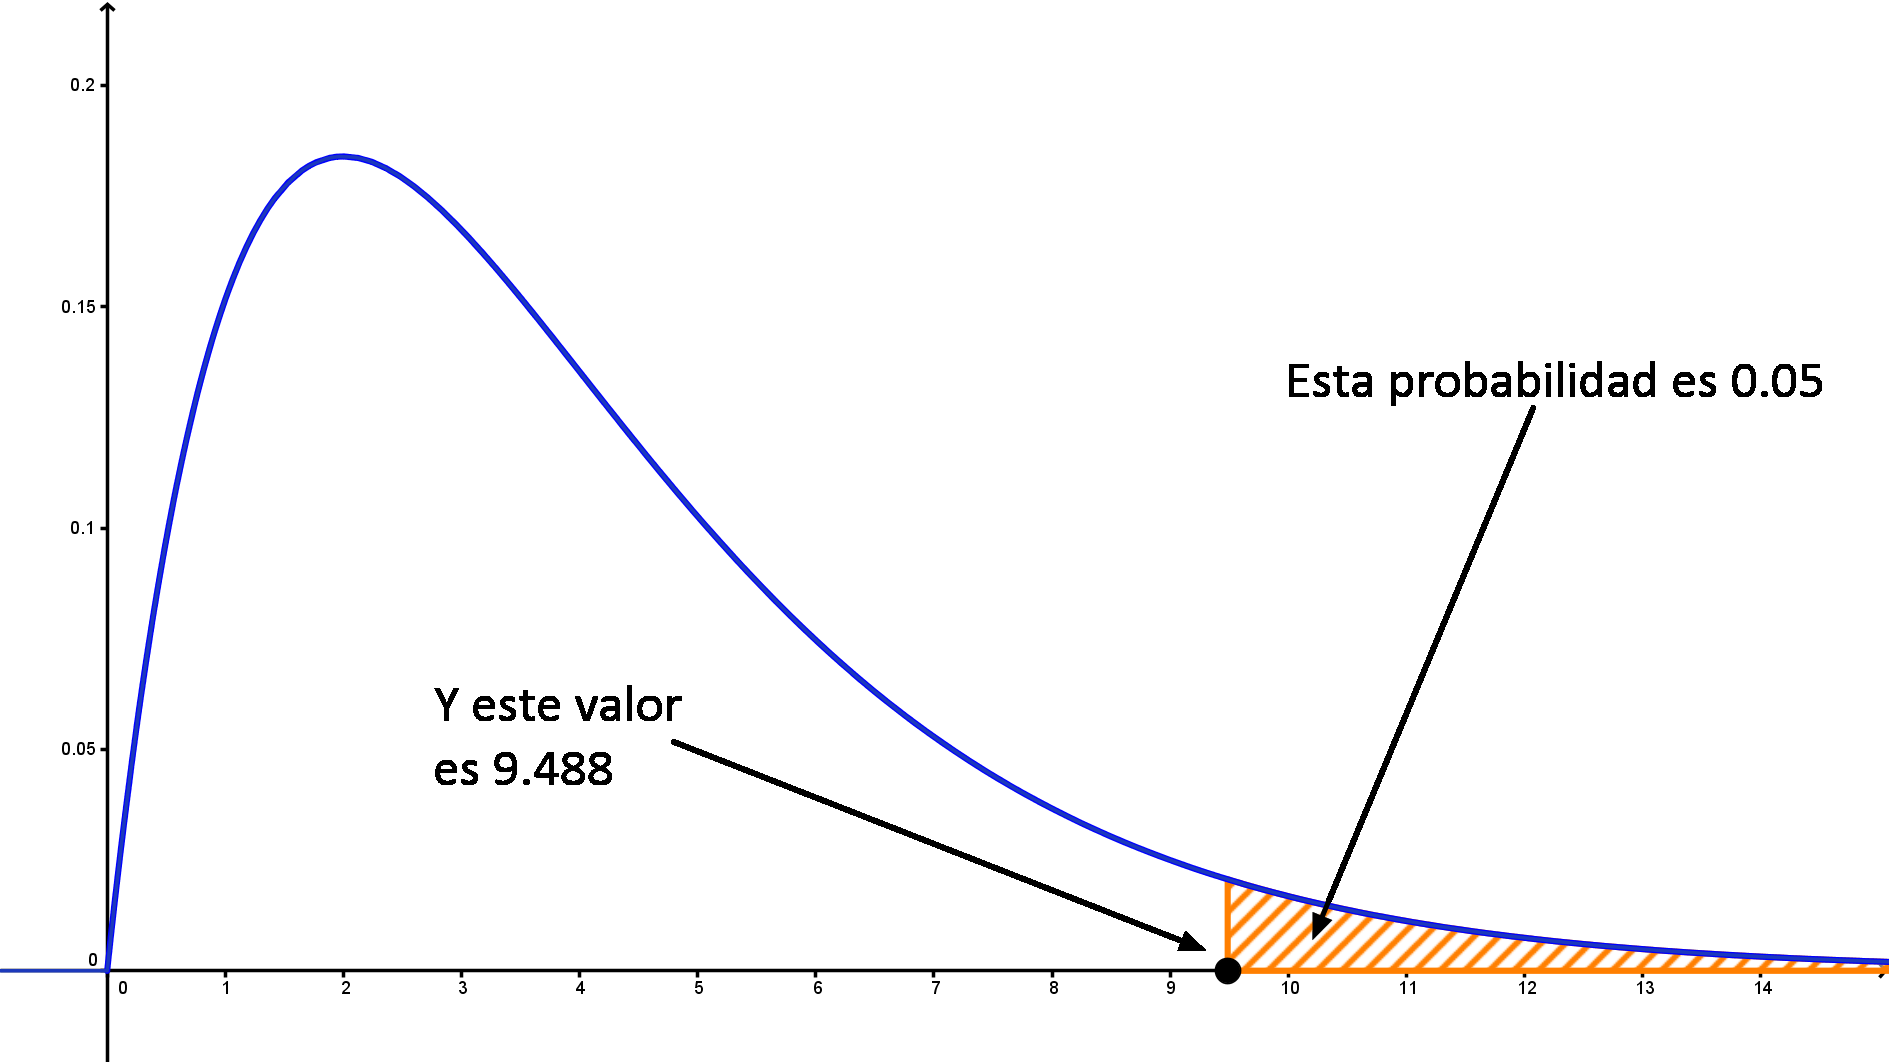
\includegraphics[width=13cm]{../fig/Cap06-ChiCuadradoProblemaInversoDerecha.png}
\end{enColor}
\begin{bn}
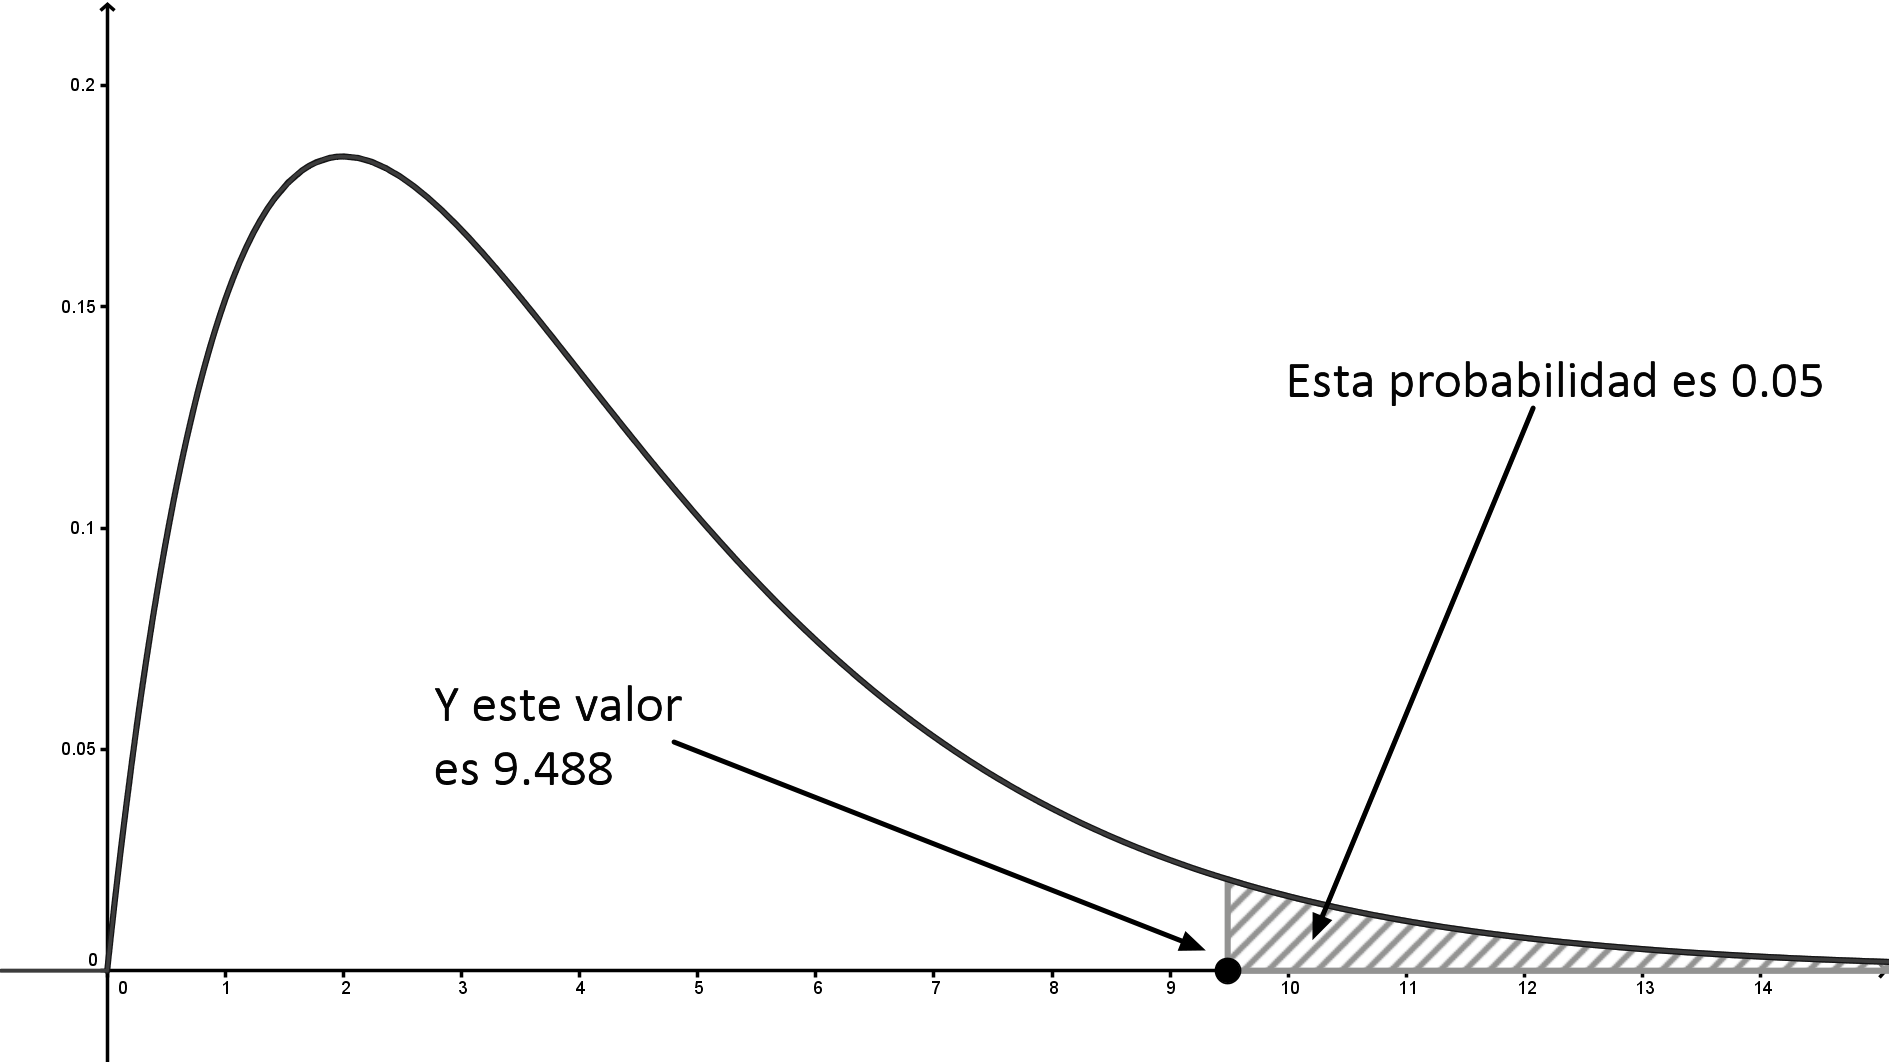
\includegraphics[width=13cm]{../fig/Cap06-ChiCuadradoProblemaInversoDerecha-bn.png}
\end{bn}
\caption{Problema inverso de probabilidad ($p_0=0.05$) para $\chi^2_4$, cola derecha.}
\label{cap06:fig:ChiCuadradoProblemaInversoDerecha}
\end{center}
\end{figure}
\end{ejemplo}

En el Tutorial06 veremos más ejemplos de este tipo, y aprenderemos a usar el ordenador para
resolver cualquier problema, directo o inverso, relacionado con la distribución $\chi^2$. Pero en
cualquier caso, la conclusión de estos ejemplos es la que avanzábamos antes: en esta distribución,
hay que trabajar cada una de las dos colas por separado. Y, si siempre es recomendable, en este
caso es casi imprescindible que el lector se acostumbre a acompañar sus razonamientos de una
pequeña figura, que le ayude a centrar las ideas y a pensar con claridad cuál es el valor que se
está calculando en cada momento.

En lo que se refiere a la notación para los cuartiles, vamos a esforzarnos en
ser coherentes, y usaremos el mismo criterio que ya hemos empleado con $Z$ y la
$t$ de Student (y que vamos a mantener durante todo el curso).

    \begin{center}
    \fcolorbox{black}{Gris025}{
    \begin{minipage}{12.5cm}
        \begin{center}
        %%%%%%%%%%%%%%%%%%%%%%%%%%%%%%%%%%%%%%%
        {\bf  Cuantiles de la distribución $\chi^2$.}\\
        \end{center}
        \index{distribución $\chi^2$, cuantiles.}\index{cuantiles de $\chi^2$}
        \index{$\chi^2$}
       %%%%%%%%%%%%%%%%%%%%%%%%%%%%%%%%%%%%%%%
       Si la variable aleatoria $Y$ tiene una distribución de tipo $\chi^2_k$, y $p_0$ es un valor cualquiera de probabilidad entonces $\chi^2_{k,p_0}$ es el valor que verifica:
       \begin{equation}\label{cap06:ecu:CuantilesChiCuadrado}
           P(Y>\chi^2_{k,p_0})=p_0.
       \end{equation}
       es decir que deja probabilidad $p_0$ en su cola derecha, o lo que es lo mismo:
       \[P(Y<\chi^2_{k,p_0})=1-p_0,\]
       deja probabilidad $1-p_0$ en su cola izquierda.
       %%%%%%%%%%%%%%%%%%%%%%%%%%%%%%%%%%%%%%%
    \end{minipage}}
    \end{center}

\subsection{Intervalo de confianza para la varianza $\sigma^2$.}
\label{cap06:subsec:IntervaloConfianzaVarianza}

Ahora que disponemos de la información necesaria sobre la distribución
$\chi^2_k$, podemos volver al problema de construir intervalos de confianza
para $\chi^2$. Combinando los resultados de la Ecuación
\ref{cap06:ecu:ObtenerDistribucionCuasivarianzaMuestral} (pág.
\pageref{cap06:ecu:ObtenerDistribucionCuasivarianzaMuestral}) con la definición
de la distribución $\chi^2$, tenemos toda la información que necesitamos. En
particular, podemos determinar cuál es el estadístico adecuado para este
problema.
    \begin{center}
    \fcolorbox{black}{Gris025}{
    \begin{minipage}{12.5cm}
        \begin{center}
        %%%%%%%%%%%%%%%%%%%%%%%%%%%%%%%%%%%%%%%
        {\bf  Estadístico para la distribución muestral de $\sigma^2$, poblaciones normales.}\\
        \end{center}
       %%%%%%%%%%%%%%%%%%%%%%%%%%%%%%%%%%%%%%%
       Si $X$ es una variable aleatoria de tipo $N(\mu,\sigma)$), y se utilizan muestras aleatorias de tamaño $n$, entonces:
       \begin{equation}\label{cap06:ecu:EstadisticoParaSigmaCuadrado}
           (n-1)\dfrac{s^2}{\sigma^2}\sim\chi^2_k,\mbox{ con }k=n-1.
       \end{equation}
       %%%%%%%%%%%%%%%%%%%%%%%%%%%%%%%%%%%%%%%
    \end{minipage}}
   \end{center}
A partir de aquí, la construcción del intervalo sigue la misma idea que ya
hemos usado en el caso de la media: como queremos un nivel de confianza
$nc=1-\alpha$, ponemos $\alpha/2$ en cada una de las dos colas de $\chi^2_k$, y
buscamos los valores críticos correspondientes, que son $\chi^2_{k,1-\alpha/2}$
y $\chi^2_{k,\alpha/2}$, como muestra la Figura
\ref{cap06:fig:ChiCuadradoValoresCriticosIntervalo}.

\begin{figure}[htb]
\begin{center}
\begin{enColor}
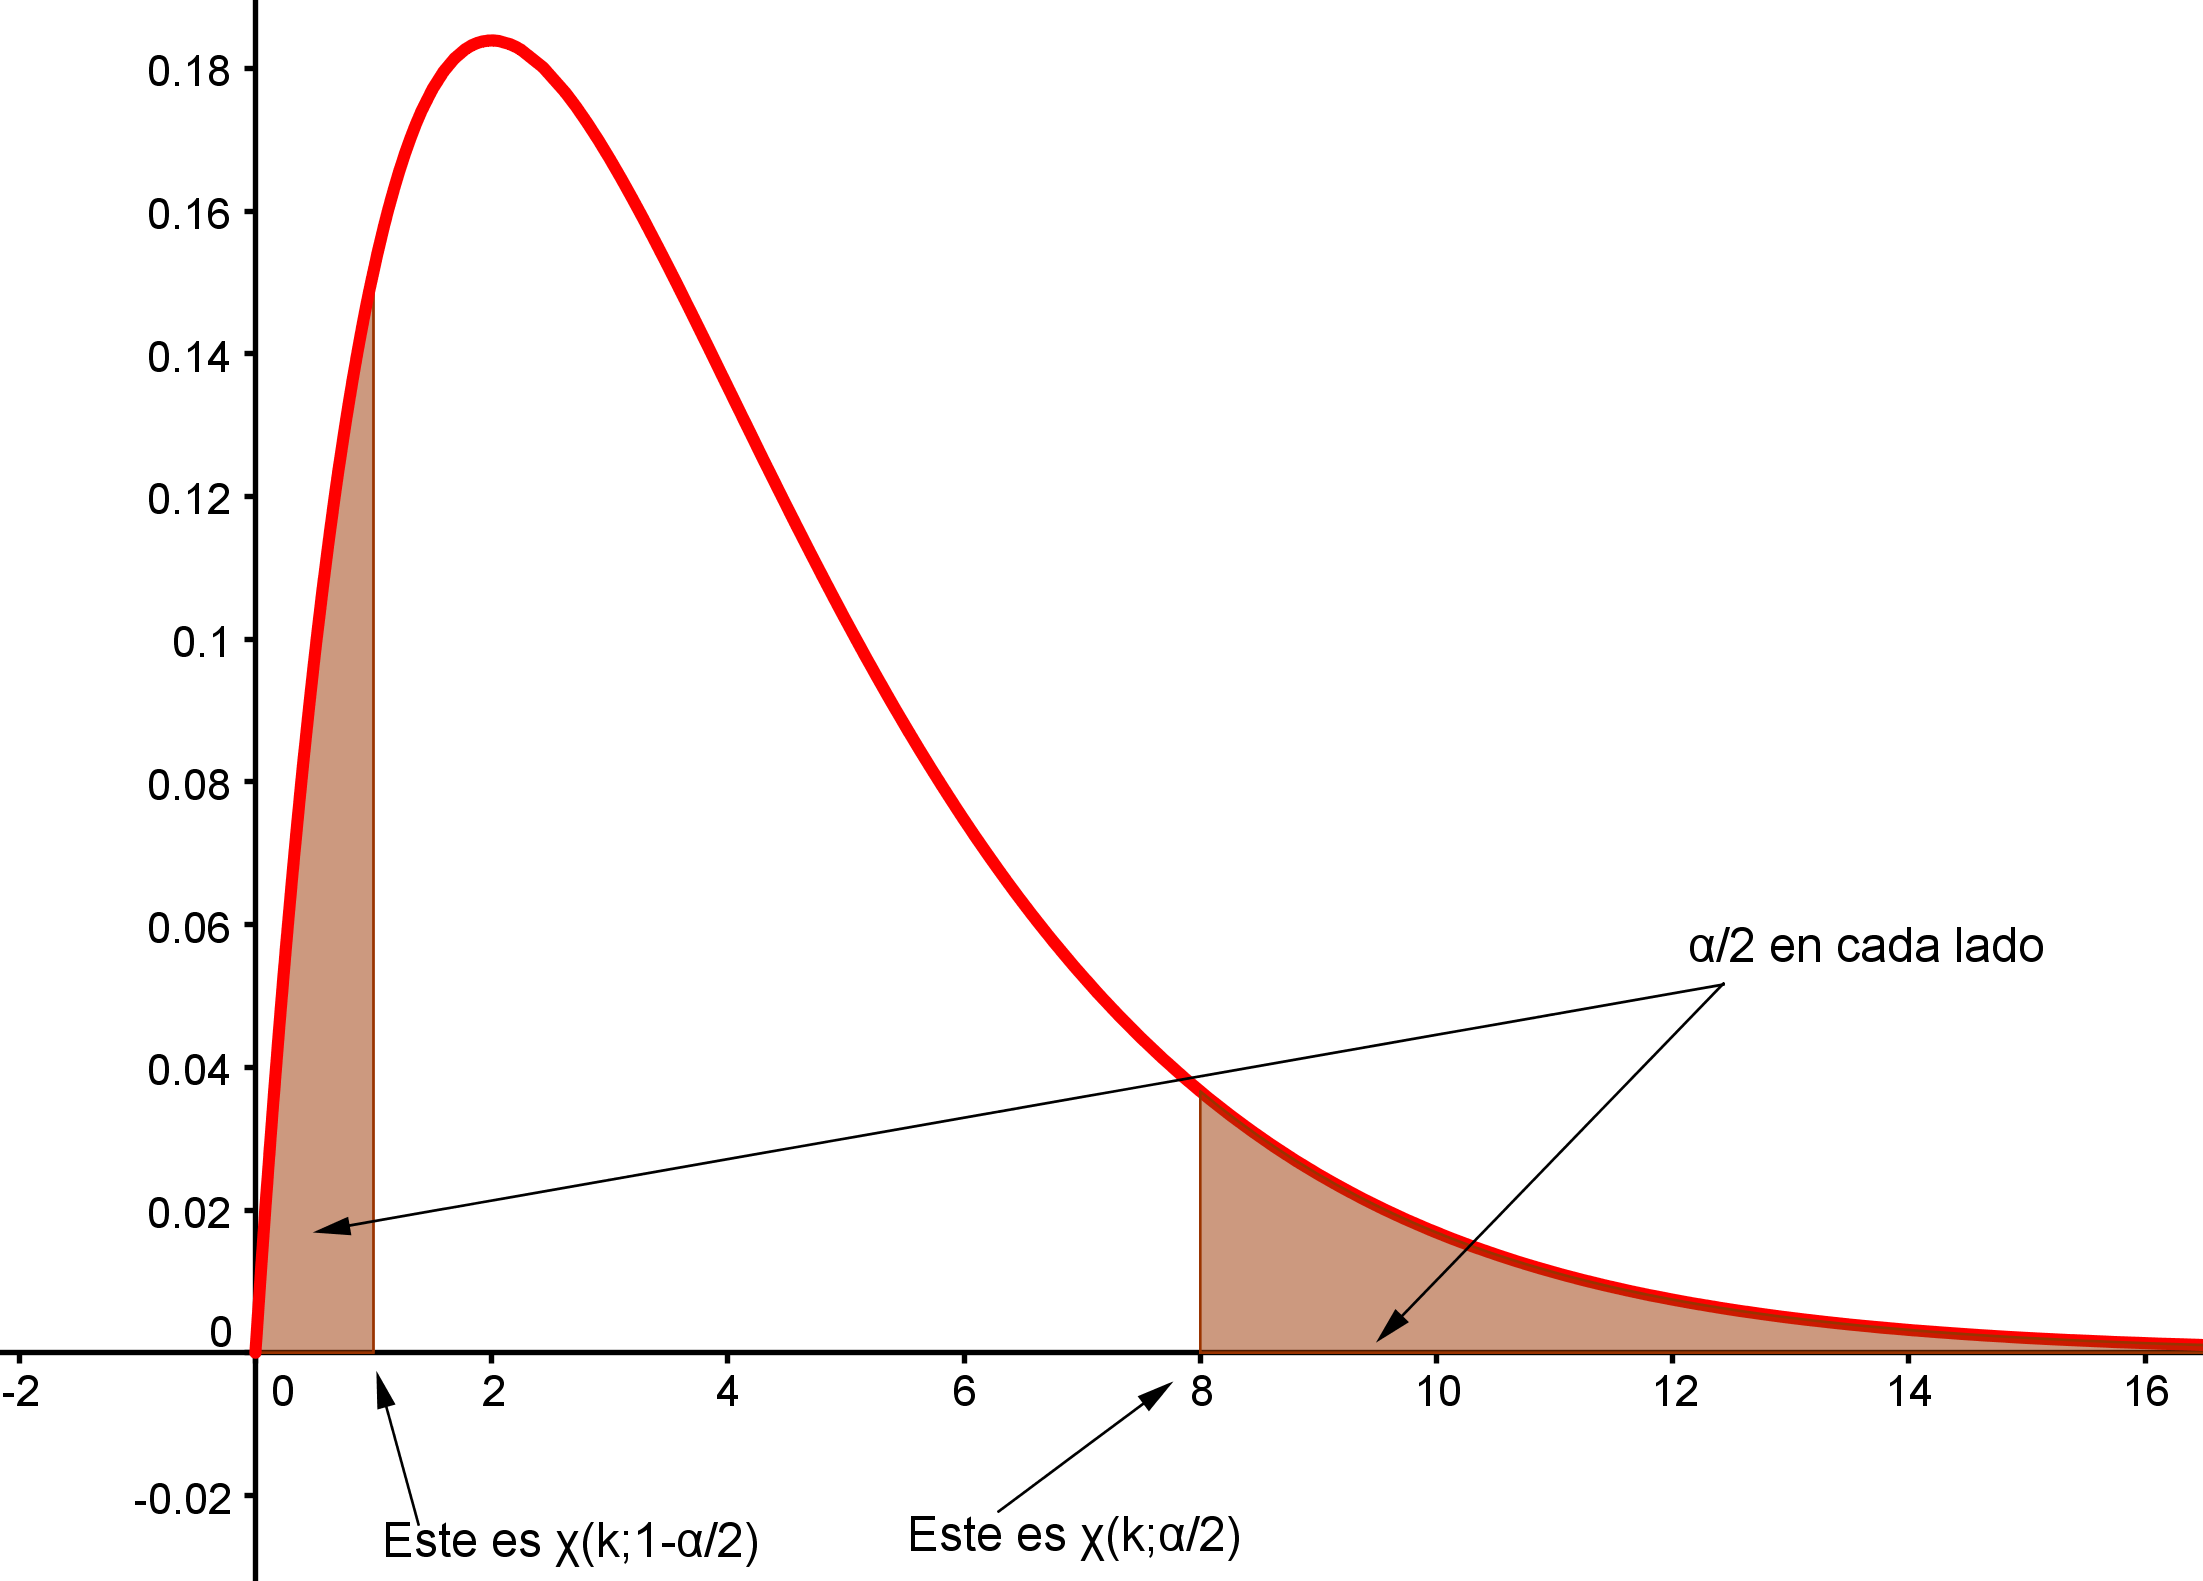
\includegraphics[width=13cm]{../fig/Cap06-ChiCuadradoValoresCriticosIntervalo.png}
\end{enColor}
\begin{bn}
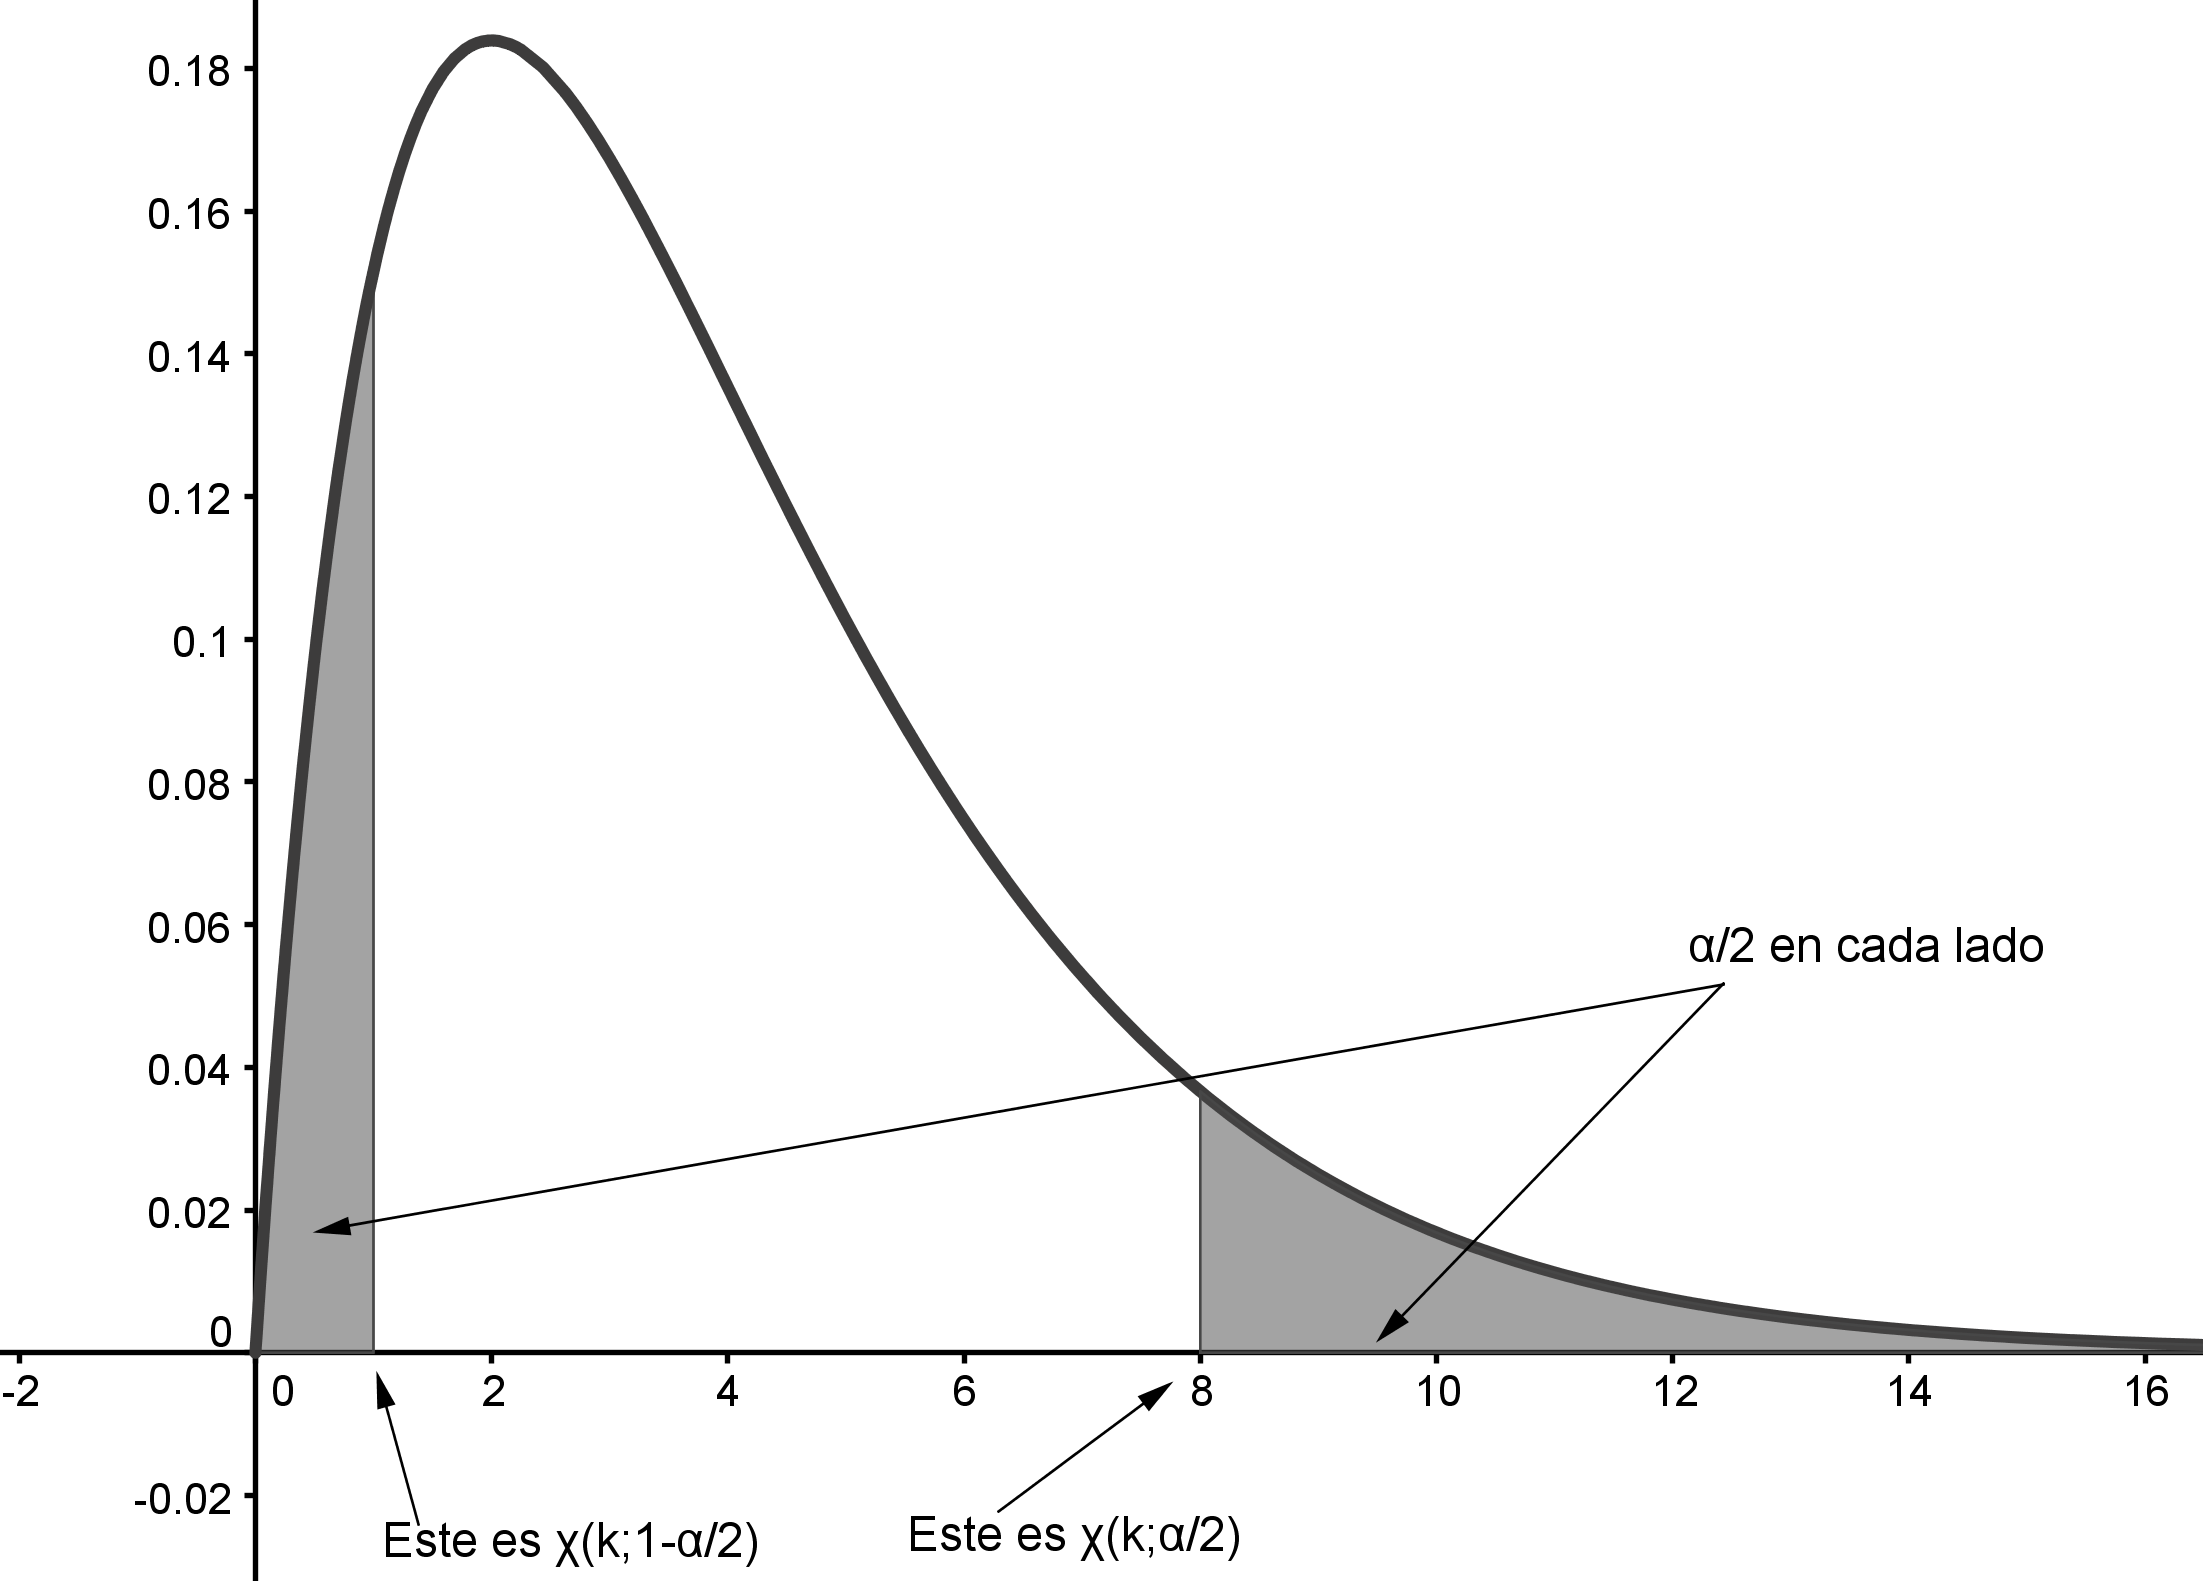
\includegraphics[width=13cm]{../fig/Cap06-ChiCuadradoValoresCriticosIntervalo-bn.png}
\end{bn}
\caption{Valores críticos en la construcción de un intervalo de confianza para $\sigma^2$, usando $\chi^2_k$.}
\label{cap06:fig:ChiCuadradoValoresCriticosIntervalo}
\end{center}
\end{figure}

Con esto hemos garantizado que:
    \[P(\chi^2_{k,1-\alpha/2}<\chi^2_k<\chi^2_{k,\alpha/2})=1-\alpha\]
Y aquí vamos a sustituir el estadístico adecuado, que es:
    \[(n-1)\dfrac{s^2}{\sigma^2}\sim\chi^2_k.\]
Obtenemos:
    \[P\left(\chi^2_{k,1-\alpha/2}<(n-1)\dfrac{s^2}{\sigma^2}<\chi^2_{k,\alpha/2}\right)=1-\alpha\]
y ahora podemos despejar $\sigma^2$ en estas desigualdades, teniendo en cuenta
que al dar la vuelta a la fracción, las desigualdades también se invierten:
    \[P\left(
    \dfrac{1}{\chi^2_{k,\alpha/2}}<\dfrac{\sigma^2}{(n-1)s^2}<\dfrac{1}{\chi^2_{k,1-\alpha/2}}
    \right)=1-\alpha.
    \]
Finalmente, despejando $\sigma^2$ en el centro de las desigualdades:
    \[P\left(
    \dfrac{(n-1)s^2}{\chi^2_{k,\alpha/2}}<\sigma^2<\dfrac{(n-1)s^2}{\chi^2_{k,1-\alpha/2}}
    \right)=1-\alpha,\]
Este es el intervalo de confianza al nivel $nc=1-\alpha$ que andábamos
buscando.

    \begin{center}
    \fcolorbox{black}{Gris025}{
    \begin{minipage}{12.5cm}
        \begin{center}
        %%%%%%%%%%%%%%%%%%%%%%%%%%%%%%%%%%%%%%%
        {\bf Intervalo de confianza (nivel $(1-\alpha$)) para $\sigma^2$ y $\sigma$, población normal.}
           \index{intervalo de confianza para la varianza}
        \end{center}
       %%%%%%%%%%%%%%%%%%%%%%%%%%%%%%%%%%%%%%%
       Sea $X$ una variable aleatoria de tipo $N(\mu,\sigma)$), y supongamos que se utilizan muestras aleatorias de tamaño $n$. Entonces el intervalo de confianza al nivel $(1-\alpha)$  para $\sigma^2=\sigma^2_X$  es (ver la Ecuación \ref{cap06:ecu:CuantilesChiCuadrado}, pág. \pageref{cap06:ecu:CuantilesChiCuadrado}, para la definición de $\chi^2_{k,p_0}$):
       \begin{equation}\label{cap06:ecu:IntervaloConfianzaVarianza}
       \dfrac{(n-1)s^2}{\chi^2_{k,\alpha/2}}\leq\sigma^2\leq\dfrac{(n-1)s^2}{\chi^2_{k,1-\alpha/2}} ,\mbox{ con }k=n-1.
       \end{equation}
       Y, por lo tanto, el intervalo de confianza para la desviación típica es:
       \begin{equation}\label{cap06:ecu:IntervaloConfianzaDesviacionTipica}
       \sqrt{\dfrac{(n-1)s^2}{\chi^2_{k,\alpha/2}}}\leq\sigma\leq\sqrt{\dfrac{(n-1)s^2}{\chi^2_{k,1-\alpha/2}}}.
       \end{equation}
       %%%%%%%%%%%%%%%%%%%%%%%%%%%%%%%%%%%%%%%
    \end{minipage}}
    \end{center}
Algunos comentarios sobre estos resultados:
\begin{itemize}
  \item Insistimos en algo que ya hemos dicho: al calcular los cuartiles
      $\chi^2_{k,\alpha/2}$, es muy recomendable utilizar una figura, como la
      Figura \ref{cap06:fig:ChiCuadradoValoresCriticosIntervalo}, para que
      nos sirva de guía.
  \item El intervalo que vamos a obtener no es, en general, simétrico. Es
      decir, $s^2$, la cuasivarianza muestral, no estará en el centro del
      intervalo, y el intervalo {\sf no se puede escribir} en la forma
      $\sigma^2=s^2\pm$(algo).
  \item Además, en este caso en particular, hay que extremar la precaución,
      porque el cuartil que calculamos usando la cola {\em izquierda} de
      $\chi^2_k$ se utiliza para calcular el extremo {\em derecho} del
      intervalo de confianza, y viceversa. En caso de confusión, recuerda
      siempre que estás calculando un intervalo de la forma:
      \[a<\sigma^2<b\]
      y, en particular, tiene que ser $a<b$. Si obtienes $a>b$, revisa tu
      trabajo, para localizar el error.
\end{itemize}

\begin{ejemplo}
\label{cap06:ejem:IntervaloConfianzaVarianzaLatasConserva}
    Una fabrica produce latas de conservas. Una muestra de 30 latas ha dado como resultado un peso
    medio de 203.5 gramos, con una cuasidesviación típica muestral de 2.6 gramos. Hallar un intervalo de confianza (al 95\%) para la desviación típica del peso de las latas que provienen de esa fábrica.

   Tenemos $k=30-1=29$. Como $1-\alpha=0.95$, es $\alpha=0.05$, con lo que $\alpha/2=0.025$ y
   $1-\alpha/2=0.975$. Entonces (usando el ordenador):
   \[\chi^2_{k,1-\alpha/2}\approx 16.047, \chi^2_{k,\alpha/2}\approx 45.72\]
   Como sabemos que $s^2=(2.6)^2=6.76$, se obtiene entonces:
   \[\dfrac{29\cdot 6.76}{45.72}<\sigma^2<\dfrac{29\cdot 6.76}{16.047}\]
   o lo que es lo mismo (calculando las raíces cuadradas):
   \[ 2.07<\sigma<3.50\]
   Fíjate, en este ejemplo, en que no hemos necesitado el valor (203.5 g) de la media para obtener
   el intervalo de confianza.

   \qed
\end{ejemplo}

\subsubsection{Estimación del tamaño muestral necesario para conseguir una precisión dada al estimar $\mu$ o $\sigma$}
\label{cap06:subsubsec:EstimacionTamannoMuestralParaMediaUsandoIntConfSigma}

Hemos dejado pendiente, desde la discusión de la página
\pageref{cap06:subsubsec:DeterminacionTamannoMuestraParaMuConSigmaDesconocida}, el cálculo del
tamaño muestral necesario para obtener un intervalo de confianza con la precisión deseada, en el
caso en el que $\sigma$ es deconocida. Vamos a usar los datos del Ejemplo
\ref{cap06:ejem:IntervaloConfianzaVarianzaLatasConserva} que acabamos de ver, para ilustrar como se
puede proceder en un caso así:
\begin{ejemplo}
 \label{cap06:ejem:DeterminacionTamannoMuestraIntConfConZUsandoIntConfSigma}
Supongamos que ahora los técnicos de la fábrica del Ejemplo
\ref{cap06:ejem:IntervaloConfianzaVarianzaLatasConserva} desean calcular el tamaño muestral
necesario para conocer el peso medio de las latas, con una precisión $\delta=0.5$ gramos, y un
nivel de confianza del $95\%$. La Ecuación \ref{cap06:ecu:TamannoMuestraIntConfMediaConZ} (pág.
\pageref{cap06:ecu:TamannoMuestraIntConfMediaConZ})
    \[
     n=\left(z_{\alpha/2}\cdot\dfrac{\sigma_X}{\delta}\right)^2
    \]
combinada con la estimación
\[ 2.07<\sigma<3.50\]
que hemos obtenido en el Ejemplo \ref{cap06:ejem:IntervaloConfianzaVarianzaLatasConserva} nos
permite obtener:
    \[
     n=\left(z_{\alpha/2}\cdot\dfrac{\sigma_X}{\delta}\right)^2\approx
        \left(1.96\cdot\dfrac{3.50}{0.5}\right)^2\approx 188.2
    \]
 A la vista de este resultado, debería usarse una muestra de la menos $189$ latas de conserva, para
 garantizar la precisión deseada.
\qed
\end{ejemplo}
Fíjate en que, en este ejemplo, hemos usado el extremo superior $3.50$ del intervalo de confianza
para $\sigma$, porque es el que produce un valor más grande de $n$, y tenemos que estar seguros de
que la muestra que construimos garantiza una precisión suficiente, incluso en el caso en el que la
desviación típica se acerca al máximo valor estimado. La muestra de $30$ latas del Ejemplo
\ref{cap06:ejem:IntervaloConfianzaVarianzaLatasConserva} juega, en este caso, el papel de {\em
estudio piloto}\index{estudio piloto}\index{piloto, estudio} del que hablamos en la discusión de la
página \pageref{cap06:subsubsec:DeterminacionTamannoMuestraParaMuConSigmaDesconocida}.

\subsubsection*{Tamaño muestral para estimar $\sigma$.}

Hasta ahora, toda la discusión sobre el cálculo del tamaño muestral se ha centrado en la estimación
de $\mu$. Naturalmente, también podemos preguntarnos cuál es el tamaño muestral necesario para
estimar $\sigma$ con una precisión dada. No vamos a dar aquí los detalles técnicos, que son más
complicados en este caso, porque la propia distribución $\chi^2_k$ que usamos para calcular el
intervalo de confianza  (ver Ecuación \ref{cap06:ecu:IntervaloConfianzaDesviacionTipica}) depende
del tamaño de la muestra. El lector interesado puede empezar por leer el artículo de 1950 de de
Greenwood y Sandomire (ver referencia \cite{greenwood1950sample} de la Bibliografía), aunque debemos advertir que la discusión es bastante técnica. En Internet pueden encontrarse tablas con el tamaño de la muestra necesario para una estimación de $\sigma$ con la precisión deseada (por ejemplo, en el enlace  [\,\ref{enlace0013}\,]\label{enlace0013a} hay una de esas tablas).
%En el Tutorial06 veremos como obtener esas tablas.


\section{Intervalos de predicción.}
\label{cap06:sec:IntervalosPrediccion}
\noindent{\bf Opcional: esta sección puede omitirse en una primera lectura.}\\

En las secciones previas de este capítulo hemos aprendido a construir varios tipos de intervalos de confianza, y en los próximos capítulos añadiremos bastantes más ejemplos de ese tipo de intervalos. Pero, junto a estos, existe otro tipo de intervalos, los llamados intervalos de predicción, que resultan muy útiles en ocasiones. Veamos un ejemplo.
\begin{ejemplo}
Supongamos que estamos tratando de establecer cual es la temperatura corporal media en los adultos sanos (en todo el ejemplo nos referimos a temperatura medida por vía oral). Una muestra de 100 individuos ha dado como resultado estos valores para la media y cuasidesviación típica muestrales:
\[\bar X=37.12,\qquad s=0.91.\]
Puesto que el tamaño de la muestra es grande, podemos usar la Ecuación \ref{cap06:ecu:IntervaloConfianzaMediaMuestraGrande} (pág. \pageref{cap06:ecu:IntervaloConfianzaMediaMuestraGrande}) para construir un intervalo de confianza al 95\% para la temperatura media en la población. Se obtiene el intervalo:
\[ 36.92< \mu <  37.32\]
Este intervalo tiene la interpretación probabilística que hemos discutido en la Sección \ref{cap06:subsec:InterpretacionProbabilisticaIntervaloConfianza}, y nos permite fijar, con bastante precisión dónde está la media de la población. Al fin y al cabo, la anchura del intervalo es menor de dos décimas de grado. Y estamos hablando de una muestra de un tamaño muy pequeño (a la vez que es suficientemente grande para justificar la inferencia). Con un estudio más amplio, reduciríamos aún más la anchura de ese intervalo.

Hasta ahí, nada nuevo. Pero supongamos que, después de medir esa muestra y calcular el intervalo, medimos la temperatura de otra persona, y obtenemos $37.4\,^{\circ}\mathrm{C}$. Esa temperatura está fuera del intervalo de confianza para la media. Pero ¿hay que preocuparse? ¿Tiene fiebre esa persona? Naturalmente que no. Entonces, ¿cuáles son los valores de temperatura corporal que podemos considerar {\em anormales}? En términos prácticos: ¿cuándo llamamos al médico?

Podemos repetir preguntas similares con muchos otros parámetros fisiológicos que se miden en
pruebas analíticas. Los resultados de, por ejemplo, un análisis de sangre, contienen siempre, junto
con los valores observados en el paciente, uno intervalos de valores que se consideran {\em
normales}.  Puedes consultar esos intervalos en cualquier análisis que te hayas hecho, o en el enlace [\,\ref{enlace0014}\,]\label{enlace0014a} de la Wikipedia (en inglés).
\qed
\end{ejemplo}
La pregunta a la que queremos responder en esta sección es ¿cómo se calculan esos intervalos de
{\em valores esperables}? Para empezar, vamos a precisar cuál es la pregunta a la que queremos
contestar.

    \begin{center}
    \fcolorbox{black}{Gris025}{
    \begin{minipage}{12.5cm}
        \begin{center}
        %%%%%%%%%%%%%%%%%%%%%%%%%%%%%%%%%%%%%%%
        {\bf  Intervalo de predicción.}\\
        \end{center}
       %%%%%%%%%%%%%%%%%%%%%%%%%%%%%%%%%%%%%%%
       Si $X$ es una variable aleatoria, un {\sf intervalo (teórico) de predicción}\index{intervalo de predicción}\index{predicción, intervalo de} (en inglés, {\em prediction interval}\index{prediction interval}) con una probabilidad $p$ dada, es un intervalo $(a,b)$ tal que
       \begin{equation}\label{cap06:ecu:IntervaloTeoricoPrediccion}
           P(a<X<b)\geq p.
       \end{equation}
       %%%%%%%%%%%%%%%%%%%%%%%%%%%%%%%%%%%%%%%
    \end{minipage}}
    \end{center}
Si conocemos exactamente la distribución de la variable $X$, podemos usarla para construir un intervalo de predicción. Pero, como sabemos, a menudo no conocemos cuál es la distribución, y sólo tenemos acceso a muestras de $X$. Por esa razón hemos llamado {\em teórico} a ese intervalo de predicción. En la práctica, lo que haremos será utilizar la información muestral para {\em estimar} ese intervalo de predicción. Esas estimaciones del intervalo (teórico) de predicción se llaman a menudo, ellas mismas, intervalos de predicción.  Normalmente, ese pequeño abuso de la notación no causa confusiones.

Para intentar despejar la posible confusión entre estos intervalos y los intervalos de confianza que ya conocemos, vamos a compararlos desde otro punto de vista. Además, puesto que las variables normales son especialmente importantes, vamos a fijarnos con más detalle en ese caso particular.

En ambos casos, como no puede ser de otra manera, el punto de partida para la construcción del intervalo (de confianza o de predicción) será una muestra aleatoria de valores de la variable $X$; sean:
\[x_1, x_2,\ldots, x_n.\]
Al construir un intervalo de confianza, por ejemplo para la media $\mu$ de $X$ y a un nivel de confianza $nc=0.95$, la pregunta a la que queremos responder es {\em ¿dónde está $\mu$?} Y es importante prestar atención al hecho de que $\mu$ no es una cantidad aleatoria, sino una característica fija de la población. Es decir, $\mu$ vale lo que vale, y si tomamos más valores muestrales de $X$, $\mu$ seguirá valiendo lo mismo. En cambio, cuando construimos (estimamos) un intervalo de predicción con una probabilidad del $95\%$, la pregunta que tratamos de responder es {\em ¿dónde estará, con esa probabilidad, el próximo valor muestral $x_{n+1}$?} Es decir, a partir de $x_1$,\ldots,$x_n$, queremos obtener un intervalo $(a,b)$ tal que, con una probabilidad igual a $0.95$, un valor aleatorio de $X$ pertenezca a $(a,b)$.

Para empezar a pensar en cómo construir el intervalo de predicción, en una variable normal, partimos de la regla del 68-95-99, que vimos en la Ecuación \ref{cap05:ecu:Regla68-95-99Normales} (pág. \pageref{cap05:ecu:Regla68-95-99Normales}). La idea intuitiva es que para atrapar a, por ejemplo, el $95\%$ de la población, debemos situarnos en la media $\mu$, y tomar una semianchura de dos desviaciones típicas para definir el intervalo. Pero hay dos matices, claro:
\begin{itemize}
  \item Puesto que en realidad no conocemos la posición exacta de la media $\mu$, y lo mejor que tenemos para situarla es un intervalo de confianza, el resultado será un intervalo centrado en $\bar X$, pero con una semianchura mayor
  \item Y, puesto que habitualmente tampoco conocemos $\sigma$, debemos emplear $s$ en su lugar, con la condición, ya conocida, de que si la muestra es grande podremos usar $Z$, pero si es pequeña será necesario usar la $t$ de Student $T_k$ (con $k=n-1$).
\end{itemize}
Para dar una descripción un poco más detallada de la forma en que se pueden construir estos intervalos, pero sin enredarnos en demasiados detalles técnicos, vamos a suponer (como hicimos en el primer intervalo de confianza que calculamos) que conocemos $\sigma$, la desviación típica de la población. Entonces, la media muestral $\bar X$ de las muestras de tamaño $n$ sigue una distribución normal de tipo $N\left(\mu,\frac{\sigma}{\sqrt{n}}\right)$. Y puesto que $X$ es una normal de tipo $N(\mu,\sigma)$, si las restamos (recuerda la Ecuación \ref{cap05:ecu:SumaVariablesNormalesIndependientes}, pág. \pageref{cap05:ecu:SumaVariablesNormalesIndependientes}),
\[X - \bar X\]
obtendremos una normal de media $\mu - \mu =0$ y con desviación típica
\[\sqrt{\left(\dfrac{\sigma}{\sqrt{n}}\right)^2+\sigma^2}=\sigma\sqrt{1+\dfrac{1}{n}}=
\sigma\sqrt{\dfrac{n+1}{n}}.\]
Y, tipificando, obtenemos:
\[
\dfrac{X - \bar X}{\sigma\sqrt{\dfrac{n+1}{n}}}\sim N(0,1)=Z.
\]
Así que, a partir de esta relación, es fácil construir la siguiente expresión del intervalo de predicción con probabilidad $p$:
\begin{equation}
\label{cap06:ecu:IntervaloPrediccionSigmaConocida}
    X = \bar X \pm z_{p/2}\sqrt{n+1}\dfrac{\sigma}{\sqrt{n}}
\end{equation}
Si comparas esta expresión con la del intervalo de confianza, con nivel de confianza $nc=1-\alpha$ (ver la Ecuación \ref{cap06:ecu:IntervaloConfianzaMediaSigmaConocida}, pág. \pageref{cap06:ecu:IntervaloConfianzaMediaSigmaConocida}), verás que cuando $p=nc$, el intervalo de predicción es siempre más ancho que el de confianza, por la presencia del factor $\sqrt{1+n}$, y de acuerdo con lo que predecía nuestra intuición.

Veamos un ejemplo, con los mismos datos del Ejemplo \ref{cap06:ejem:IntConfMediaSigmaConocida} (pág. \pageref{cap06:ejem:IntConfMediaSigmaConocida}).
\begin{ejemplo}
\label{cap06:ejem:IntPrediccionSigmaConocida}
   Recordemos que en el Ejemplo \ref{cap06:ejem:IntConfMediaSigmaConocida} teníamos
   \[n=50, \quad \bar X=320,\quad \sigma=4.\]
   Y allí, usando que
   \[z_{\alpha/2}=2.58,\]
   obtuvimos este intervalo de confianza al $99\%$ para la media de la población:
   \[318.54\leq \mu_X\leq 321.46,\mbox{ es decir, }\mu=320\pm 1.46.\]
   Para obtener el intervalo de predicción en este caso, usamos $p=0.99$, y entonces, naturalmente:
   \[z_{p/2}=2.58.\]
   El uso del valor, y la interpretación del intervalo cambian, pero este valor, que es un cuantil de $Z$, no cambia según la interpretación que le demos. Con esto, sustituyendo en la Ecuación \ref{cap06:ecu:IntervaloPrediccionSigmaConocida} se obtiene el intervalo de predicción:
   \[ 309.6 < X < 330.4 \]
   que, como puede comprobarse, es sensiblemente más ancho que el intervalo de confianza.

   Para ilustrar el significado de ambos intervalos, hemos hecho una simulación (veremos cómo hacerla en el Tutorial06), en la que hemos generado $10000$ valores aleatorios de esta población, y hemos contado cuantos de ellos pertenecen al intervalo de predicción, y cuantos al de confianza.  Al intervalo de predicción pertenecen $9901$ de los $10000$ valores generados, ligeramente por encima del $99\%$ estipulado. En cambio, al intervalo de confianza sólo pertenecen $2020$ de esos valores, como cabía esperar.
\qed
\end{ejemplo}

En una situación más realista, la desviación típica de la población será desconocida, y a veces las muestras serán pequeñas. En esos casos, mientras la hipótesis de normalidad de la población se mantenga, se puede usar el siguiente resultado, que se obtiene con una manipulación un poco más complicada que la que hemos hecho. Fíjate en que se usa $s$ como sustituto de $\sigma$, y la $t$ de Student en lugar de la $Z$.
    \begin{center}
    \fcolorbox{black}{Gris025}{
    \begin{minipage}{12.5cm}
        \begin{center}
        %%%%%%%%%%%%%%%%%%%%%%%%%%%%%%%%%%%%%%%
        {\bf Intervalo de predicción con probabilidad $p$ para una población normal, con varianza desconocida.}
           \index{intervalo de predicción, población normal, con varianza desconocida}
        \end{center}
       %%%%%%%%%%%%%%%%%%%%%%%%%%%%%%%%%%%%%%%
       Dada una muestra de tamaño $n$ de una variable normal, con media muestral $\bar X$ y cuasidesviación típica muestral $s$, un intervalo de predicción con probabilidad $p$ viene dado por:
        \begin{equation}
        \label{cap06:ecu:IntervaloPrediccionSigmaDesconocida}
            X = \bar X \pm t_{k;p/2}\sqrt{n+1}\dfrac{s}{\sqrt{n}}=
            \bar X \pm t_{k;p/2}s\sqrt{1+\dfrac{1}{n}}
        \end{equation}
        %%%%%%%%%%%%%%%%%%%%%%%%%%%%%%%%%%%%%%%
    \end{minipage}}
    \end{center}
La segunda forma es la que aparece en la mayoría de los textos que se ocupan de los intervalos de predicción. Volveremos a encontrarnos con los intervalos de predicción en el Capítulo \ref{cap:RegresionLinealSimple}, en el contexto de los modelos de regresión lineal.


\section{Muestra aleatoria simple. Función de verosimilitud.}
\label{cap06:sec:MuestraAleatoriaSimpleFuncionVerosimilitud}
\noindent{\bf Opcional: esta sección puede omitirse en una primera lectura.}\\

En la pág. \pageref{cap06:ecu:MediaMuestral} hemos dicho que una muestra aleatoria
simple de tamaño $n$\index{muestra aleatoria simple} de la variable $X$ es una lista $(X_1,X_2,\ldots,X_n)$           de $n$ copias {\sf independientes} de la variable $X$. Es decir, con el lenguaje de las Secciones \ref{cap04:sec:IndependenciaVariablesAleatoriasDiscretas} y \ref{cap05:sec:VectoresAleatoriosContinuos}, la muestra aleatoria simple es un vector aleatorio. Vamos a ver lo que significa la definición de muestra aleatoria simple, en términos de la función de densidad conjunta $f_{(X_1,\ldots,X_n)}$ de ese vector aleatorio.

Supongamos que $f_X(x)$ es la función de densidad de la variable $X$  (para el caso discreto, ver la Ecuación \ref{cap04:ecu:funcionDensidadVariableAleatoriaDiscreta}, pág. \pageref{cap04:ecu:funcionDensidadVariableAleatoriaDiscreta}; para el caso continuo, ver la Sección \ref{cap05:sec:MasDetallesSobreDistribucionesContinuas}, pág. \pageref{cap05:sec:MasDetallesSobreDistribucionesContinuas}). Entonces al decir que $X_1, \ldots, X_n$ son copias de $X$, lo que estamos diciendo es que las distribuciones marginales:
\[f_{X_1}(x_1),\,f_{X_1}(x_2),\,\ldots,\,f_{X_n}(x_n)\]
son todas iguales a $f_X(x)$. En símbolos:
\[f_{X_i}(x) = f_{X}(x),\quad\mbox{ para cualquier $i$ y cualquier $x$.}\]
Y la independencia significa entonces que la función de densidad conjunta es el producto de esas densidades marginales:
\begin{equation}
\label{cap06:ecu:FuncionDensidadConjuntaMuestraAleatoriaSimple}
f_{(X_1,\ldots,X_n)}(x_1,x_2,\ldots,x_n)=
f_{X_1}(x_1)\cdot f_{X_2}(x_2)\cdot\,\cdots\, f_{X_1}(x_1)=
\end{equation}
\[= f_{X}(x_1)\cdot f_{X}(x_2)\cdot\,\cdots\, f_{X}(x_1).\]
Observa que en el último término hemos eliminado los subíndices de las distribuciones marginales para insistir en la idea de que son todas las misma función $f_X$.

Vamos a ver en un ejemplo de cómo funciona esto para las variables de tipo {\em Bernouilli$(p)$}.
\begin{ejemplo}
\label{cap06:ejem:FuncionDensidadConjuntaMuestraAleatoriaSimpleBernouilli}
La función de densidad de una variable $X$ de tipo $Bernoulli(p)$ es
(ver Ecuación \ref{cap05:ecu:FuncionDensidadVariableBernouilli}, pág. \pageref{cap05:ecu:FuncionDensidadVariableBernouilli}):
\[
f_X(x)=p^{x}\cdot q^{1-x}.
\]
Así que si tomamos una muestra aleatoria simple $(X_1,\ldots,X_n)$ de la variable $X$, su función de densidad conjunta es, según la Ecuación \ref{cap06:ecu:FuncionDensidadConjuntaMuestraAleatoriaSimple}:
\[
f_{(X_1,\ldots,X_n)}=
f_{X}(x_1)\cdot f_{X}(x_2)\cdot\,\cdots\, f_{X}(x_1)=
(p^{x_1}\cdot q^{1-x_1})\cdot (p^{x_1}\cdot q^{1-x_1})\cdot\,\cdots\,\cdot(p^{x_n}\cdot q^{1-x_n})
.
\]
Y, agrupando los términos, esto es igual a:
\[
f_{(X_1,\ldots,X_n)}(x_1,x_2,\ldots,x_n)=
p^{\sum_{i=1}^n x_i}\cdot q^{n-\sum_{i=1}^n x_i}.
\]
Así que, por ejemplo, si tenemos $p=\dfrac{1}{5}$, y observamos una muestra aleatoria simple de tamaño $3$, con valores $(X_1,X_2,X_3)=(1,1,0)$, se tendría:
\[
f_{(X_1,X_2,X_3)}(1,1,0)=
\left(\dfrac{1}{5}\right)^{1+1+0}\cdot \left(\dfrac{4}{5}\right)^{3-(1+1+0)}=\dfrac{4}{5^3}.
\]
\qed
\end{ejemplo}

\subsubsection{Función de verosimilitud.}
\label{cap06:subsubsec:FuncionVerosimilitud}

Los anteriores resultados sobre muestras aleatorias simples nos permiten dar una descripción mucho más precisa de la idea de función de verosimilitud $\cal L$, que encontramos en el Capítulo \ref{cap:Probabilidad} (ver la pág. \pageref{cap03:subsubsec:verosimilitud}). En aquel capítulo vimos, de manera informal, que la verosimilitud estaba relacionada con la probabilidad de los datos que usamos para verificar una teoría. Muchas veces, las teorías se pueden expresar como afirmaciones o hipótesis sobre el valor de un cierto parámetro (en el Capítulo \ref{cap:ContrasteHipotesis} volveremos con mucho más detalle sobre esta idea general de lo que es someter a prueba una teoría). Un ejemplo extremadamente simple, en el caso del lanzamiento de una moneda de la que sospechamos que está cargada,  puede ser la teoría ``la probabilidad de cara es $\frac{1}{5}$ (en lugar de $\frac{1}{2}$)''. Fíjate en que en este caso la teoría se refiere al valor del parámetro $p$ de una variable de tipo $Bernouilli(p)$. ¿Cómo podríamos comprobar esa teoría? Evidentemente, lanzaríamos la moneda unas cuantas veces. Es decir, tomaríamos una muestra de la variable. Por eso no es de extrañar que el contexto adecuado para definir la función $\cal L$ sea el de las muestras aleatorias simples, que son el modelo teórico de una recogida de datos.
    \begin{center}
    \fcolorbox{black}{Gris025}{
    \begin{minipage}{12cm}
        \begin{center}
        {\bf Función de verosimilitud de una muestra aleatoria simple.}
        \end{center}
        \index{función de verosimilitud de una muestra aleatoria simple}
        \index{verosimilitud, función de (muestra aleatoria simple)}
        Sea $X$ una variable aleatoria que depende de un parámetro $\theta$, con función de densidad $f_X(x;\theta)$, y sea $(X_1,\ldots,X_n)$ (el vector aleatorio que define) una muestra aleatoria simple de $X$. Entonces la {\sf función de verosimilitud ${\cal L}$} de esa muestra es la función:
        \begin{equation}
        \label{cap04:ecu:FuncionVerosimilitudMuestraAleatoriaSimple}
        {\cal L}(x_1,\ldots,x_n;\theta)=
        f_{(X_1,\ldots,X_n)}(x_1,x_2,\ldots,x_n;\theta)=
        \end{equation}
        \[
        = f_{X}(x_1;\theta)\cdot f_{X}(x_2;\theta)\cdot\, \cdots \,\cdot f_{X}(x_1;\theta).
        \]
    \end{minipage}}
    \end{center}
Aquí $f_{(X_1,\ldots,X_n)}(x_1,x_2,\ldots,x_n;\theta)$ es la función de densidad conjunta de la muestra, y hemos usado la Ecuación \ref{cap06:ecu:FuncionDensidadConjuntaMuestraAleatoriaSimple} para escribirla como un product de copias de $f_X$. La notación pretende destacar el hecho de que estamos considerando $f$ {\em también} como una función del parámetro $\theta$. Esa es precisamente la diferencia entre $\cal L$ y la función de densidad conjunta. En la densidad conjunta pensamos en $\theta$ como un valor {\em fijo}, mientras que en $\cal L$ estamos pensando explícitamente en $\theta$ como variable, mientras que  $x_1,\ldots,x_n$ representan los valores muestrales (que se pueden considerar fijos).

\begin{ejemplo}{\bf (Continuación del Ejemplo \ref{cap06:ejem:FuncionDensidadConjuntaMuestraAleatoriaSimpleBernouilli}).}
\label{cap06:ejem:FuncionDensidadConjuntaMuestraAleatoriaSimpleBernouilli-2}
En el caso de una variable $X$ de tipo $Bernouilli(p)$, el parámetro $\theta$ es la probabilidad $p$ de éxito. Las distintas ``teorías'' que podemos construir en este caso son afirmaciones sobre el  valor de $p$. Una teoría puede sostener, como hicimos en el Ejemplo \ref{cap06:ejem:FuncionDensidadConjuntaMuestraAleatoriaSimpleBernouilli}, que es $p=\dfrac{1}{5}$. Y podemos tratar de usar muestras aleatorias simples de la variable $X$ para poner a prueba esa teoría.

Usando los resultados de ese Ejemplo \ref{cap06:ejem:FuncionDensidadConjuntaMuestraAleatoriaSimpleBernouilli}, podemos decir directamente que, para una muestra aleatoria simple de una variable $X$ de tipo $Bernouilli(p)$, se cumple:
\[
{\cal L}(x_1,x_2,\ldots,x_n;p)=
p^{\sum_{i=1}^n x_i}\cdot q^{n-\sum_{i=1}^n x_i}.
\]
Supongamos, por ejemplo, que hemos lanzado la moneda $n=100$ veces, y que hemos obtenido $20$ veces cara  (éxito) y $80$ veces cruz. Eso significa que, en esa muestra,
\[\sum_{i=1}^n x_i = 20,
\]
y, por lo tanto, la verosimilitud $\cal L$ de esa muestra, vista como función de $p$ es:
\[
{\cal L}(x_1,x_2,\ldots,x_n;p) = p^{20}\cdot q^{80} = p^{20}\cdot (1-p)^{80}.
\]
La Figura \ref{cap06:fig:FuncionVerosimilitudEjemploBernouilli} muestra esa función de verosimilitud para todos los valores posibles de $p$ en el intervalo $[0,1]$ (el eje vertical está en millonésimas). A la vista de los resultados muestrales, no debería resultar sorprendente que el valor donde la función verosimilitud alcanza el máximo corresponda a $p=\dfrac{20}{100}=\dfrac{1}{5}$.
\begin{figure}[h!]
\begin{center}
\begin{enColor}
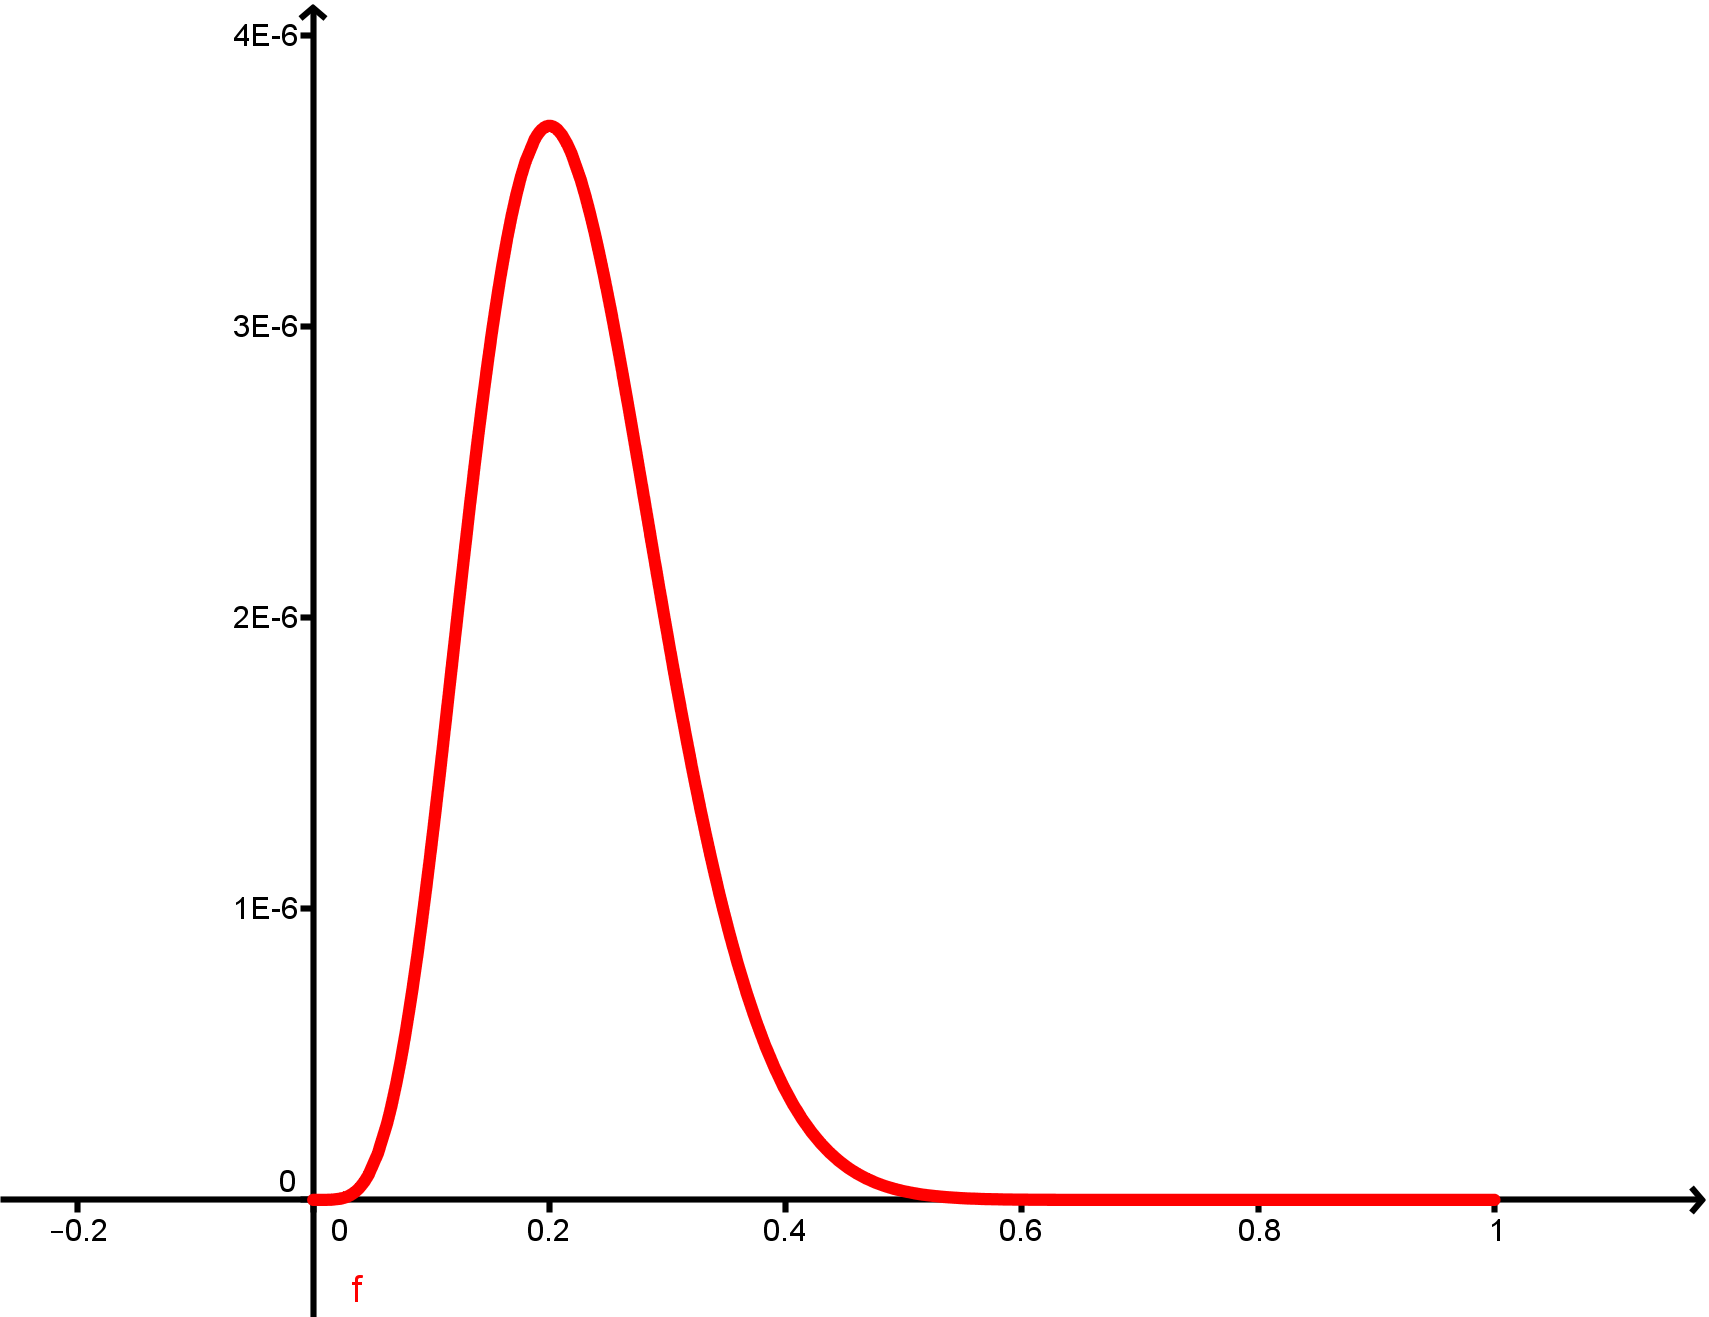
\includegraphics[height=5cm]{../fig/Cap06-FuncionVerosimilitudEjemploBernouilli.png}
\end{enColor}
\begin{bn}
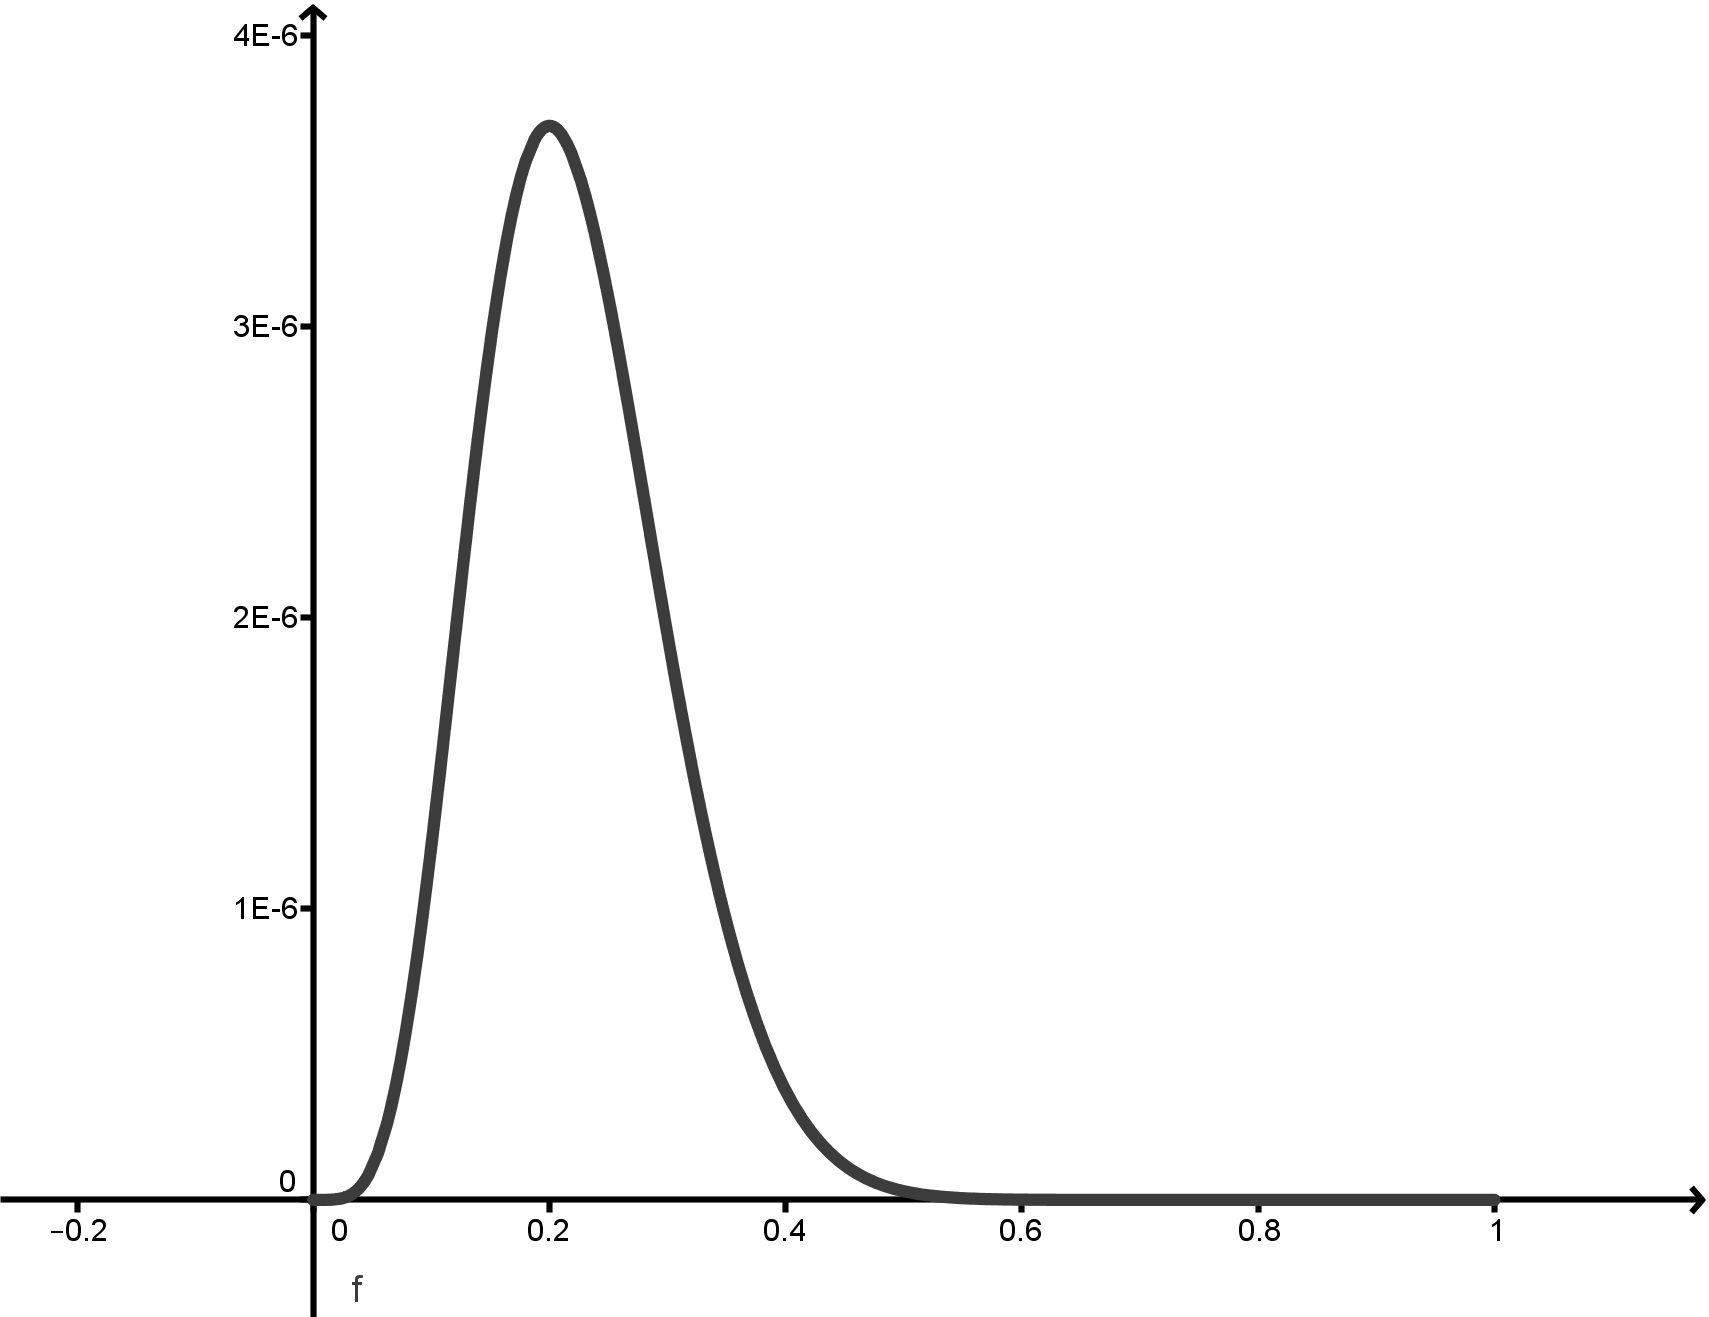
\includegraphics[height=5cm]{../fig/Cap06-FuncionVerosimilitudEjemploBernouilli-bn.png}
\end{bn}
\caption{Función de verosimilitud $\cal L$ del Ejemplo \ref{cap06:ejem:FuncionDensidadConjuntaMuestraAleatoriaSimpleBernouilli-2}.}
\label{cap06:fig:FuncionVerosimilitudEjemploBernouilli}
\end{center}
\end{figure}
Una manera de interpretar este resultado es que $p=1/5$ es el valor que hace más probables los datos que hemos observado.
\qed
\end{ejemplo}
